\documentclass[12pt]{report}
\usepackage{mathptmx}
\usepackage{graphicx}
\usepackage[authoryear]{natbib}
\usepackage{float}
\usepackage{subcaption}
\usepackage{amsmath,amssymb}
\usepackage{url}
\usepackage{hyperref}
\usepackage{booktabs}
\usepackage{multirow}
\usepackage{geometry}
\geometry{a4paper, margin=1in}
\setlength{\emergencystretch}{2em}
\graphicspath{{figures/}}

\begin{document}
\hypersetup{pageanchor=false}

% ═══════════════════════════════════════════════════════════════
%  TITLE PAGE
% ═══════════════════════════════════════════════════════════════
\begin{titlepage}
    \centering
    \vspace*{2cm}
    {\Large\bfseries Study of Cosmic Void Size Function using Computational Methods:\\[6pt]
    Validation with Simulated Catalogs, Bayesian Parameter Estimation,\\[4pt]
    and Lessons in Model Calibration\par}
    \vspace{1.5cm}
    {\Large\itshape Arun Mitra Kommireddy\\ 2021B5A42443H \par}
    \vfill
    {\large Submitted in partial fulfillment of the requirements\\
    for the course BITS F422T: FD Thesis (16U)\\[6pt]
    \bfseries Birla Institute of Technology and Science, Pilani\par}
    \vspace{1cm}
    {\large Supervised by:\\\bfseries Prof.\ Federico Marulli, University of Bologna, Italy\\ Dr. Simone Sartori, Aix-Marseille University, France\\ Prof.\ Ram Chandra Murthy Kalluri, Birla Institute of Technology and Science Pilani, Hyderabad, India\par}
    \vfill
    {\large 7th May, 2026\par}
\end{titlepage}

% ═══════════════════════════════════════════════════════════════
%  ACKNOWLEDGMENTS
% ═══════════════════════════════════════════════════════════════
\chapter*{Acknowledgments}
\addcontentsline{toc}{chapter}{Acknowledgments}

I thank Prof.\ Federico Marulli for supervising this work and for helping me shape it into a coherent research project. His comments during our weekly clustering meetings were especially useful when I was trying to distinguish pipeline bugs from genuine modelling problems. I am also grateful to Dr.\ Simone Sartori for guiding me through the BitVF workflow, the cleaning prescription, and the logic behind the reference catalogues used in this thesis. His own thesis and his responses to many technical questions were directly useful throughout this project.

I thank Prof.\ Sashideep Gutti and Prof.\ Ram Chandra Murthy Kalluri for their support and advice during the thesis. Their encouragement helped me keep the work moving even when the validation and MCMC stages became more complicated than I had initially expected.

I also benefited from the work of Dr.\ Sofia Contarini and Dr.\ Tommaso Ronconi, especially in understanding how the Void Size Function is used for cosmological inference and why calibration matters before interpreting posteriors. The discussions and reviews within the clustering group were equally helpful; they repeatedly pushed me to check assumptions more carefully and to make the limitations of the analysis explicit.

I am grateful to all of them for making it possible for me to work on this problem in a serious research setting.

\bigskip\noindent Thank you.

% ═══════════════════════════════════════════════════════════════
%  TABLE OF CONTENTS
% ═══════════════════════════════════════════════════════════════
\tableofcontents
\hypersetup{pageanchor=true}
\clearpage

% ═══════════════════════════════════════════════════════════════
%  ABSTRACT
% ═══════════════════════════════════════════════════════════════
\chapter*{Abstract}
\addcontentsline{toc}{chapter}{Abstract}

We investigate the Void Size Function (VSF) as a cosmological probe by examining vast underdense regions in the large-scale structure. This thesis presents a two-phase computational analysis of the VSF, running on the Aletheia $N$-body simulation ($250\;h^{-1}\mathrm{Mpc}$ box, $\Omega_m=0.315$, $\sigma_8=0.811$). First, we thoroughly validate the BitVF (Back-in-Time Void Finder) identification and cleaning pipeline, comparing it to the standard REVOLVER geometric framework across multiple tracer sparsity levels (20\%, 10\%, 5\%, 2.5\%). Our geometric pipeline applies a density threshold of $\delta_\mathrm{avg} \leq -0.80$, strict OV00 overlap pruning, and boundary exclusion. We show that geometric VSFs shift systematically with tracer density, while the dynamical BitVF approach---which leverages divergent mass flow via displacement field reconstruction---remains far more stable.

In the second phase, we run a Bayesian MCMC parameter estimation built on the Volume-Conserving (Vdn) model \citep{Sheth2004,Jennings2013}. Using the \texttt{emcee} sampler \citep{ForemanMackey2013}, we float $\Omega_m$, $\sigma_8$, and the void formation threshold $\delta_v$. Crucially, our pre-MCMC validation uncovers a severe model-data tension: at the true Aletheia cosmology, the Vdn model overpredicts small-radius ($R \lesssim 5\;h^{-1}\mathrm{Mpc}$) void abundance by a factor of 2--5. This tension breaks the MCMC, driving $\Omega_m$ to the prior floor (0.10) in all runs, even as $\sigma_8$ stays marginally recoverable for the Optimal Transport reconstructed (NREC50) field. 

These findings emphasize that a robust void-finding pipeline alone is insufficient; rigorous theoretical calibration is absolutely essential before extracting cosmology from void statistics. Our work lays the necessary diagnostic foundation for upcoming void analyses in surveys like BOSS, DESI, and Euclid.

% ═══════════════════════════════════════════════════════════════
%  CHAPTER 1: INTRODUCTION
% ═══════════════════════════════════════════════════════════════
\chapter{Introduction}

\section{Context and Motivation}

The $\Lambda$CDM standard model has achieved remarkable success in describing the Universe, matching observations ranging from the Cosmic Microwave Background (CMB) to the clustering of galaxies \citep{Planck2020}. Yet, the era of precision cosmology demands independent cross-checks, particularly given persisting tensions in fundamental parameters like $H_0$ and $S_8$. Alternative probes of the large-scale structure do not replace traditional measurements; rather, they offer complementary leverage on the same underlying physics.

Cosmic voids are particularly compelling in this regard. Taking up the vast majority of the Universe's volume, voids represent the underdense tail of the matter distribution. While dense galaxy clusters undergo complex, non-linear collapse heavily influenced by baryonic physics, voids simply expand outward. This expansion keeps them closer to the quasi-linear regime for much longer, making their dynamical evolution cleaner to model. 

My thesis focuses on the Void Size Function (VSF) to ask a highly practical question: does the VSF remain a stable, reliable cosmological observable after we run it through the messy reality of void identification and cleaning pipelines? This immediately brings us face-to-face with the algorithmic realities of tracer sparsity, void overlap, boundary effects, and model mapping.

\section{The Void Size Function as a Cosmological Observable}

An important statistical metric of void populations is the Void Size Function (VSF), defined as the number density of voids as a function of their effective radius:
\begin{equation}
    \frac{dn}{d\ln R_v}
    \label{eq:vsf_definition}
\end{equation}
where $n$ is the comoving number density and $R_v$ is the effective void radius. Analogous to the halo mass function for overdense structures, the VSF encodes information about the growth of cosmic structure and is sensitive to fundamental cosmological parameters, principally the matter density parameter $\Omega_m$ and the amplitude of density fluctuations $\sigma_8$.

Excursion-set theory underpins our ability to predict the VSF, originally developed by \citet{Bond1991} to describe the abundance of dark matter haloes within the Press--Schechter framework \citep{PressSchechter1974}. This formalism was extended to voids by \citet{Sheth2004}, who introduced a two-barrier model that accounts for the competition between void formation (at the linear underdensity threshold $\delta_v \approx -2.71$, corresponding to shell crossing) and the collapse of surrounding overdense regions (at $\delta_c \approx 1.686$). The resulting Sheth--van de Weygaert (SvdW) multiplicity function describes the fraction of the cosmic volume occupied by voids of a given scale, incorporating the ``void-in-cloud'' process whereby small voids embedded within larger collapsing regions are erased during structure formation.

Building upon this framework, \citet{Jennings2013} introduced the Volume-Conserving model (Vdn), which improves the mapping between Lagrangian (initial) and Eulerian (final) void radii by enforcing total volume conservation. This correction addresses an inconsistency in the original excursion-set prediction and yields improved agreement between theoretical predictions and $N$-body simulations at large void radii.

Even with these theoretical leaps, the models assume idealised voids that are spherical, non-overlapping, and defined by a fixed enclosed density contrast (commonly $\delta_\mathrm{NL} \approx -0.8$). Translating observational or simulated data into such idealised objects is non-trivial and requires careful methodological treatment, as we describe in subsequent sections.


\section{The Algorithmic Challenge: Identifying Voids in Tracer Space}

In practice, voids are not identified directly in the underlying continuous matter field but in discrete tracer distributions such as galaxies or dark matter haloes. Most widely used void-finding algorithms, including ZOBOV \citep{Neyrinck2008} and its implementation in REVOLVER \citep{Nadathur2019}, operate on the tracer density field using Voronoi tessellation and watershed transformations to identify underdense regions.

However, this introduces a fundamental limitation: void identification is performed in \emph{tracer space}, not in the true matter field. These methods implicitly assume that gaps in the tracer distribution correspond to genuine underdensities in the mass distribution. This assumption breaks down under realistic conditions due to two principal effects:

\begin{itemize}
    \item \textbf{Tracer sparsity:} Observational surveys and simulated catalogues provide only a finite, sparse sampling of the underlying density field. When the mean particle separation becomes comparable to or larger than the characteristic size of small voids, random fluctuations in tracer positions create artificial empty regions that are indistinguishable from genuine underdensities. These spurious detections predominantly affect the small-radius regime of the VSF, leading to an artificial enhancement in void abundance.

    \item \textbf{Tracer bias:} Galaxies and haloes are biased tracers of the matter distribution, clustering preferentially in overdense environments. This biased spatial distribution distorts the apparent density field: regions between clusters may appear empty in tracer space while containing significant matter density. The linear bias parameter $b$ relates the tracer density contrast to the matter density contrast via $\delta_g \approx b \cdot \delta_m$, but this simple relation breaks down on scales relevant to void interiors.
\end{itemize}

These effects lead to significant systematic variations in the resulting void catalogues and, consequently, in the inferred VSF. \citet{Nadathur2015a} demonstrated that void properties depend sensitively on survey characteristics, while \citet{Contarini2019} showed that tracer bias significantly affects the size and abundance of detected voids. These findings raise fundamental questions about the extent to which void statistics derived from tracer-based catalogues can be considered robust cosmological observables.


\section{The Role of Post-Processing and Cleaning}

A further complication arises from the mismatch between the theoretical void definitions assumed by models like the Vdn framework and the algorithmic output of watershed-based void finders. The raw output of ZOBOV-type algorithms consists of irregular, nested, and overlapping basins that bear little resemblance to the idealised spherical, non-overlapping voids assumed in excursion-set theory.

To resolve this, we must apply a cleaning pipeline to transform raw watershed basins into a physically meaningful population of voids. The standard cleaning procedure, as developed and validated in the void cosmology literature \citep{Ronconi2017,Contarini2019,Contarini2023,Sartori2025}, involves several sequential steps:

\begin{enumerate}
    \item \textbf{Density threshold:} Voids are required to satisfy a mean enclosed density contrast below a specified threshold, typically $\delta_\mathrm{avg} \leq -0.80$. This ensures that only genuinely underdense structures are retained.

    \item \textbf{Overlap removal:} Overlapping voids are pruned to ensure statistical independence. In the strict ``OV00'' criterion used in this work, two voids are considered overlapping if the distance between their centres is less than the sum of their radii ($D_{ij} < R_i + R_j$), and the smaller void is removed.

    \item \textbf{Boundary treatment:} Voids whose centres lie within a specified distance of the survey boundary (typically $20\;h^{-1}\mathrm{Mpc}$) are removed to avoid biases from incomplete volume coverage.
\end{enumerate}

This cleaning process enables a consistent mapping between observed voids and theoretical expectations, making the VSF a meaningful cosmological observable. However, it also introduces an important conceptual subtlety: the final void population is not purely observational but is partly defined through methodological choices, and these choices can influence the inferred cosmology.


\section{From Geometric to Dynamical Void Definitions}

While geometric void finders provide a practical and well-tested starting point, their sensitivity to tracer properties motivates the exploration of fundamentally different approaches. Dynamical void finders aim to reconstruct the underlying matter field using displacement or velocity information, thereby decoupling the void definition from the static tracer density.

The conceptual foundation for this approach traces back to \citet{Brenier2003}, who formulated the reconstruction of the initial conditions of the Universe as a convex optimisation (optimal transport) problem. Building on this framework, \citet{Eisenstein2007} developed density field reconstruction techniques for baryon acoustic oscillation (BAO) measurements, demonstrating the practical feasibility of recovering the large-scale displacement field from galaxy distributions.

The Back-in-Time Void Finder (BitVF), introduced by \citet{Sartori2025}, applies these ideas directly to void identification. BitVF identifies voids as regions of \emph{divergent mass flow}, namely locations where the reconstructed displacement field diverges outward, rather than as purely geometric underdensities in tracer space. By operating closer to the underlying matter distribution, this approach is expected to be more robust to tracer sparsity and bias, representing a shift from descriptive to physically motivated void definitions.

In the BitVF framework, two types of displacement fields can be employed:
\begin{itemize}
    \item \textbf{True Displacement Field (BIT):} The exact displacement vectors from the simulation, representing the ideal case with no reconstruction noise.
    \item \textbf{Optimal Transport Reconstructed Field (NREC50):} Displacements reconstructed from tracer positions using 50 iterations of the optimal transport algorithm, representing the realistic scenario applicable to observational data.
\end{itemize}

This work builds on this transition from geometric to dynamical methods, using geometric approaches as a baseline and systematically investigating the extent to which dynamical methods mitigate known systematic effects.


\section{Cosmological Parameter Estimation from the VSF}
\label{sec:intro_mcmc}

Beyond measuring the void population, the VSF can be fitted with a theoretical model and used to infer cosmological parameters. In practice, this means building a forward model, evaluating it at the same radius bins as the data, defining a likelihood, and then sampling the posterior over parameters such as $\Omega_m$ and $\sigma_8$.

This procedure is only meaningful if the forward model and the measured data vector are actually compatible at a known cosmology. That point is easy to state, but it turns out to be the main issue in this thesis. Observational analyses such as \citet{Contarini2023} address it by calibrating the model against mock catalogues processed through the same void-finding and cleaning pipeline. That step is not optional bookkeeping; it determines whether the posterior is tracing cosmology or compensating for model error.

In this work, I implement the MCMC layer using the Vdn model and the \texttt{emcee} sampler \citep{ForemanMackey2013,GoodmanWeare2010}. The important result is not that the chains run. It is that the pre-MCMC validation already shows structured disagreement between the model and the measured VSF, and the later posterior behaviour simply exposes the consequences of ignoring that mismatch.


\section{Scope and Objectives of This Work}

The objective of this thesis is narrower and more practical than a general study of void cosmology. I want to know whether the pipeline I built can reproduce the intended cleaned VSF, and whether the resulting data vector is already suitable for cosmological inference with a simple analytical model.

\paragraph{Phase 1: Pipeline Validation.} I implement the cleaning and VSF pipeline for the BitVF catalogues, compare the output against the Simone\_data reference files, and test how the result changes across the four Aletheia tracer subsamples. This stage is meant to answer a concrete question: if the final VSF differs from the reference, is the cause in my cleaning code or earlier in the catalogue-generation chain?

\paragraph{Phase 2: MCMC Parameter Estimation.} I then use the cleaned VSF as input to a Vdn-based MCMC analysis. Here the main question is again practical: does the forward model already match the data well enough at the true cosmology for the posterior to be trusted? The answer, as the later chapters show, is no.

The value of the thesis therefore lies in separating two issues that are often conflated. A pipeline can be technically correct and still produce a data vector that is not yet ready for unbiased parameter inference. Much of the discussion that follows is built around making that distinction explicit.


% ═══════════════════════════════════════════════════════════════
%  CHAPTER 2: THEORETICAL BACKGROUND AND LITERATURE REVIEW
% ═══════════════════════════════════════════════════════════════
\chapter{Theoretical Background and Literature Review}

\section{The Cosmic Web and the Role of Cosmic Voids}

The large-scale structure of the Universe is shaped by the gravitational evolution of primordial density fluctuations, resulting in a hierarchical network commonly referred to as the cosmic web \citep{Bond1991,VanDeWeygaert2011}. This intricate structure consists of dense galaxy clusters connected by elongated filaments and planar sheets, surrounding vast underdense regions known as cosmic voids. Among these components, voids are unique in that they occupy most of the cosmic volume, with estimates ranging from 70\% to 90\% \citep{VanDeWeygaert2011}, while containing only a small fraction of the total mass.

The dynamical evolution of voids differs fundamentally from that of overdense structures. While clusters and filaments form through gravitational collapse, attracting matter from their surroundings, voids expand as matter flows outward towards surrounding overdensities. This expansion occurs in a quasi-linear regime: the density contrast within voids remains moderate ($-1 < \delta < 0$), meaning that perturbation theory provides a reasonable description of their internal dynamics even at late cosmic times. In contrast, overdense structures quickly enter the nonlinear regime where perturbative approaches fail, and complex baryonic physics (gas cooling, star formation, feedback from active galactic nuclei) further complicates the connection between theory and observation.

This relative simplicity makes voids particularly attractive as cosmological probes. Their sensitivity extends to several key aspects of fundamental physics:

\begin{itemize}
    \item \textbf{Dark energy:} The expansion rate of voids is directly sensitive to the dark energy equation of state $w$, as dark energy influences both the background expansion history and the growth rate of structure. In void interiors, the dark-energy-to-matter density ratio is enhanced relative to the cosmic mean, amplifying the observable signatures \citep{Pisani2015,Pisani2019MNRAS}.

    \item \textbf{Modified gravity:} Alternative theories of gravity predict different void profiles and expansion rates compared to General Relativity. The low-density environment of voids provides a natural laboratory for testing screening mechanisms, which suppress modifications to gravity in high-density regions but allow them to operate in underdense environments \citep{Li2012,Contarini2021}.

    \item \textbf{Neutrino mass:} Massive neutrinos, due to their large free-streaming length, preferentially fill voids rather than clustering with cold dark matter. The presence of massive neutrinos therefore modifies the void density profile and abundance, providing a complementary probe of the neutrino mass sum $\sum m_\nu$ \citep{Massara2015,Contarini2021}.

    \item \textbf{CMB lensing:} Voids create convergence troughs in the CMB lensing signal, which have been detected observationally. Recent work using the DESI Legacy Survey has demonstrated the measurement of void imprints on CMB lensing maps \citep{Aubert2024}, opening a new multi-probe channel for void cosmology.
\end{itemize}

Over the past decade, the field has matured rapidly, with cosmic voids increasingly recognised as a first-class cosmological probe alongside galaxy clustering, weak lensing, and the CMB \citep{Pisani2019WhitePaper,Moresco2022,Hamaus2023}.


\section{The Void Size Function as a Statistical Observable}

The core metric used to describe of void populations is the Void Size Function (VSF), defined as the comoving number density of voids as a function of their effective radius, $dn/d\ln R_v$ (Equation~\ref{eq:vsf_definition}). This function serves as the underdense counterpart to the halo mass function and encodes information about the distribution and evolution of large-scale structure.

The theoretical prediction of the VSF is rooted in the excursion-set formalism. In this framework, the density field is smoothed on progressively larger scales, and a random walk in the smoothed density contrast $\delta(R)$ as a function of the smoothing scale $R$ is analysed. Structures form when the random walk first crosses a specified density threshold: $\delta_c \approx 1.686$ for halo collapse and $\delta_v \approx -2.71$ for void shell crossing (in the linear regime).

\citet{Sheth2004} extended this formalism to voids by introducing a two-barrier excursion-set model. The key physical insight is that void formation is not simply the mirror image of halo formation: small underdense regions embedded within larger collapsing overdensities are compressed and erased rather than expanding into voids. This ``void-in-cloud'' process introduces a second barrier (the collapse threshold $\delta_c$) that suppresses the formation of small voids.

The resulting SvdW multiplicity function captures this competition between the two barriers and provides the probability that a random region of the Universe will evolve into a void of a given size. \citet{Jennings2013} subsequently introduced the Volume-Conserving (Vdn) model, which corrects the Lagrangian-to-Eulerian mapping by enforcing that the total volume occupied by voids is preserved. This correction addresses an inconsistency in the original formulation and yields improved agreement with numerical simulations.

More recently, \citet{Paranjape2024} have sought to unify the treatment of overdense and underdense structures within a common framework through a universal multiplicity function, while \citet{Verza2024} introduced a moving-barrier model with scale-dependent thresholds calibrated on simulations, achieving percent-level accuracy in predicting the VSF. These developments represent the state of the art in theoretical void modelling.

Despite these advances, all analytical models share common assumptions that limit their direct applicability: they assume idealised voids that are spherical, non-overlapping, and characterised by a single enclosed density contrast. Real voids identified by algorithms are irregular, often nested, and defined through algorithmic procedures that introduce their own systematics.


\section{The Volume-Conserving (Vdn) Theoretical Model}
\label{sec:vdn_model}

The Vdn model, which serves as the forward model for the MCMC parameter estimation in this work, combines the SvdW multiplicity function with a volume-conserving Lagrangian-to-Eulerian mapping. We present the key equations here; implementation details are given in Appendix~\ref{app:vdn_implementation}.

\subsection{The SvdW Multiplicity Function}

The \citet{Sheth2004} two-barrier multiplicity function gives the fraction of cosmic volume in voids of a given scale. The void barrier is defined at the linear shell-crossing threshold $\delta_v$, and the cloud barrier at the linear collapse threshold $\delta_c = 1.686$. The multiplicity function takes the form of an infinite series:
\begin{equation}
    f(\sigma) = 2 \sum_{j=1}^{\infty} \exp\!\left[-\frac{(j\pi x)^2}{2}\right]\, j\pi x^2 \,\sin(j\pi D)
    \label{eq:svdw}
\end{equation}
where the auxiliary variables are defined as:
\begin{equation}
    D = \frac{|\delta_v|}{|\delta_v| + \delta_c}\,, \qquad
    x = \frac{D\,\sigma}{|\delta_v|}
\end{equation}
Here $\sigma \equiv \sigma(R_L)$ is the root-mean-square linear density fluctuation on the Lagrangian scale $R_L$, computed from the matter power spectrum $P(k)$:
\begin{equation}
    \sigma^2(R) = \frac{1}{2\pi^2}\int_0^\infty k^2\,P(k)\,\hat{W}^2(kR)\,dk
    \label{eq:sigma_R}
\end{equation}
where $\hat{W}(kR)$ is the Fourier transform of the top-hat window function. The series in Equation~\ref{eq:svdw} converges rapidly; we truncate it at $j=50$ terms in our implementation. The physical content of this expression is the probability that a random walk in the smoothed density field crosses the void barrier $\delta_v$ before encountering the collapse barrier $\delta_c$, naturally incorporating the void-in-cloud suppression.

\subsection{Lagrangian-to-Eulerian Mapping}

Voids expand from their initial Lagrangian radius $R_L$ to their present-day Eulerian radius $R_E$ via spherical evolution. In the spherical model, a region with nonlinear density contrast $\delta_\mathrm{NL}$ has expanded by:
\begin{equation}
    R_E = R_L\,(1 + \delta_\mathrm{NL})^{-1/3}
    \label{eq:lag_to_eul}
\end{equation}
With the adopted nonlinear threshold $\delta_\mathrm{NL} = -0.80$ (corresponding to the cleaning threshold used in the pipeline), the expansion factor is:
\begin{equation}
    C \equiv (1 + \delta_\mathrm{NL})^{-1/3} = (1 - 0.80)^{-1/3} \approx 1.71
\end{equation}
This expansion factor connects the theoretical predictions (which are naturally expressed in Lagrangian space) to the observed void sizes (in Eulerian space).

\subsection{The Vdn Model}

The Volume-Conserving model \citep{Jennings2013} computes the VSF as:
\begin{equation}
    \frac{dn}{d\ln R_E} = \frac{f(\sigma)}{V(R_E)}\left|\frac{d\ln\sigma^{-1}}{d\ln R_L}\right|
    \label{eq:vdn}
\end{equation}
where $V(R_E) = \frac{4}{3}\pi R_E^3$ is the Eulerian volume. The derivative $|d\ln\sigma^{-1}/d\ln R_L|$ encodes the sensitivity of the variance to the smoothing scale and is computed numerically via central finite differences.

\subsection{Physical Meaning of the Thresholds}
\label{sec:thresholds}

The model contains several density thresholds with distinct physical meanings:

\begin{itemize}
    \item $\delta_v \approx -2.71$: the \emph{linear} void formation threshold, corresponding to shell crossing in the spherical evolution model. This is the barrier in the excursion-set random walk.

    \item $\delta_c = 1.686$: the \emph{linear} halo collapse threshold, serving as the upper barrier that suppresses small voids (void-in-cloud process).

    \item $\delta_\mathrm{NL} = -0.80$: the \emph{nonlinear} enclosed density contrast used to define void boundaries in the cleaning pipeline. This parameter connects the theoretical model to the operational void definition.
\end{itemize}

The variance $\sigma(R)$ is computed using the \texttt{COLOSSUS} Python toolkit \citep{Diemer2018}, which provides the linear matter power spectrum for arbitrary cosmological parameters. This allows the Vdn model to be evaluated rapidly for different values of $\Omega_m$ and $\sigma_8$, enabling efficient MCMC sampling.


\section{Void Identification: From Continuous Fields to Discrete Tracers}
\label{sec:void_id_methods}

A major challenge in studying voids is that voids are not directly observed in the continuous matter field but rather inferred from discrete tracers such as galaxies or dark matter haloes. This introduces an inherent ambiguity: voids are not uniquely defined objects but depend on the method used to identify them. The principal methodological categories are:

\begin{enumerate}
    \item \textbf{Spherical underdensity finders:} These methods search for maximal spheres below a specified density threshold \citep{Ceccarelli2009}. While computationally simple and easy to connect to theoretical models, they cannot capture the complex, triaxial shapes that characterise real cosmic voids and therefore miss a significant fraction of the void population.

    \item \textbf{Watershed and Voronoi methods:} The current standard approach, exemplified by ZOBOV \citep{Neyrinck2008} and its wrappers such as REVOLVER \citep{Nadathur2019} and VIDE \citep{Sutter2015}. These algorithms construct a Voronoi tessellation of the tracer distribution to estimate local densities, then apply a watershed transform to identify voids as density basins. This approach preserves the natural geometry of voids without imposing a predefined shape, but introduces sensitivity to shot noise (tracer sparsity) and hierarchical merging issues \citep{Nadathur2015a}. The resulting voids are often irregular, nested, and overlapping, requiring significant post-processing to enable comparison with theoretical models.

    \item \textbf{Dynamical finders:} An emerging class of algorithms that define voids based on the dynamics of the matter field rather than the static tracer density. Methods such as DIVA \citep{Lavaux2010,Elyiv2015} and BitVF \citep{Sartori2025} reconstruct the displacement or velocity field and identify voids as regions of divergent mass flow. By operating closer to the underlying physics, these methods aim to decouple the void definition from tracer sampling effects, offering theoretical robustness against noise and bias.
\end{enumerate}

Each approach involves trade-offs between physical fidelity, computational cost, and sensitivity to observational systematics. This work primarily employs the watershed approach (via REVOLVER) as the geometric baseline and BitVF as the dynamical alternative, enabling a direct comparison of their relative robustness.


\section{The Impact of Tracer Bias and Sparsity}

A key limitation of geometric void-finding methods is their reliance on tracer distributions, which are imperfect representations of the underlying matter field. The systematic effects of tracer bias and sparsity on void statistics have been extensively studied:

\citet{Nadathur2015a} demonstrated that void properties, including size distributions, density profiles, and spatial clustering, depend sensitively on the characteristics of the tracer population, especially its number density and bias. \citet{Contarini2019} showed that tracer bias significantly affects the size and abundance of detected voids in the VIPERS survey, with implications for cosmological constraints derived from void statistics. More recently, \citet{Pollina2019} investigated the linearity of tracer bias around voids, finding that the relationship between tracer and matter density fields behaves differently in underdense environments compared to the cosmic mean.

These findings highlight a fundamental characteristic of void statistics: they are not purely physical quantities reflecting the matter distribution but are influenced by observational and methodological factors. This observation motivates the development of methods that are less sensitive to tracer properties, as well as careful calibration procedures when extracting cosmological information from void statistics.


\section{Cleaning and the Mapping to Theoretical Predictions}

To bridge the gap between algorithmically identified voids and theoretical models such as the Vdn framework, a cleaning procedure is typically applied to raw void catalogues. This process has been developed and refined through a series of methodological studies \citep{Ronconi2017,Ronconi2019,Contarini2019,Contarini2023,Sartori2025}.

The essential steps are:

\begin{enumerate}
    \item \textbf{Density filtering:} Retaining only voids whose mean enclosed density contrast satisfies $\delta_\mathrm{avg} \leq \delta_\mathrm{NL}$ (typically $-0.80$). This ensures that the void population corresponds to genuinely underdense regions consistent with the theoretical definition.

    \item \textbf{Radius rescaling:} In some implementations, void radii are rescaled to the radius at which the enclosed density contrast equals the target threshold. This enforces a consistent operational definition across the void population.

    \item \textbf{Overlap removal:} Overlapping voids are pruned to create a non-overlapping population, as assumed by excursion-set theory. Different overlap criteria exist (see Section~\ref{sec:overlap_criteria}).

    \item \textbf{Boundary correction:} Voids near survey edges are removed to avoid biases from incomplete volume coverage.
\end{enumerate}

These steps are essential for obtaining physically meaningful void catalogues, but they also introduce an important conceptual point: the final void definition is not purely observational but is partly imposed through methodological choices, and these choices propagate into the inferred cosmology. Understanding and controlling this propagation is one of the central themes of this work.


\section{Observational Measurements and the BOSS Survey}

The application of void statistics to observational data has been enabled by large galaxy redshift surveys. The Baryon Oscillation Spectroscopic Survey (BOSS), part of the Sloan Digital Sky Survey III, provides a comprehensive mapping of the large-scale structure through spectroscopic observations of over one million galaxies out to redshift $z \sim 0.7$, covering approximately 10{,}000 square degrees of sky \citep{Reid2016}.

The BOSS DR12 dataset has become a benchmark for void cosmology. \citet{Hamaus2020} used void-galaxy cross-correlations measured from BOSS to constrain the growth rate of structure, while \citet{Contarini2023} measured the Void Size Function from BOSS and derived cosmological constraints on $\Omega_m$ and $\sigma_8$. A critical ingredient in the \citeauthor{Contarini2023} analysis was the calibration of the theoretical model against mock catalogues: the same void-finding and cleaning pipeline was applied to simulated catalogues at known cosmologies, and the resulting systematic offset between theory and pipeline output was measured and corrected before performing MCMC inference on the real data. This calibration step is essential for producing unbiased cosmological constraints, as our results will further demonstrate.


\section{Bayesian Parameter Estimation for Void Cosmology}
\label{sec:bayesian_background}

The extraction of cosmological constraints from the VSF proceeds through Bayesian inference. Given a data vector $\mathbf{d}$ (the measured VSF in radial bins) and a theoretical model $\mathbf{m}(\boldsymbol{\theta})$ parameterised by cosmological parameters $\boldsymbol{\theta}$, the posterior probability distribution is given by Bayes' theorem:
\begin{equation}
    P(\boldsymbol{\theta}|\mathbf{d}) \propto \mathcal{L}(\mathbf{d}|\boldsymbol{\theta})\,\pi(\boldsymbol{\theta})
    \label{eq:bayes}
\end{equation}
where $\mathcal{L}$ is the likelihood function and $\pi(\boldsymbol{\theta})$ is the prior.

Assuming Gaussian errors, the log-likelihood takes the form:
\begin{equation}
    \ln\mathcal{L} = -\frac{1}{2}\sum_i \frac{[d_i - m_i(\boldsymbol{\theta})]^2}{\sigma_i^2}
    \label{eq:gaussian_loglike}
\end{equation}
where the sum runs over radial bins, and $\sigma_i$ represents the uncertainty in each bin. In this work, we use Poisson errors estimated from the void counts: $\sigma_i = \sqrt{N_i}/(V_\mathrm{eff}\,\Delta\ln R)$, where $N_i$ is the number of voids in bin $i$, $V_\mathrm{eff}$ is the effective survey volume, and $\Delta\ln R$ is the bin width. This diagonal covariance is a simplification; the full covariance matrix, which captures bin-to-bin correlations arising from the cleaning procedure and large-scale modes, would require an ensemble of mock realisations to estimate reliably.

The posterior is sampled using Markov Chain Monte Carlo (MCMC) methods. We employ the \texttt{emcee} package \citep{ForemanMackey2013}, which implements the affine-invariant ensemble sampler of \citet{GoodmanWeare2010}. This sampler uses an ensemble of ``walkers'' that explore the parameter space simultaneously, with proposals generated from the complementary ensemble. The affine-invariant property ensures that the sampling efficiency does not depend on the coordinate system or the shape of the posterior distribution, making it well suited for the correlated parameter spaces encountered in cosmological analyses.

A critical prerequisite for MCMC-based parameter estimation is that the forward model must accurately describe the data at the known true cosmology. If the model exhibits systematic biases, such as overpredicting or underpredicting the VSF at certain radii, the MCMC sampler will be driven to parameter values that compensate for the model deficiency rather than recovering the true cosmology. This is the calibration requirement, and its violation is a central finding of this work.


\section{Toward Dynamical Void Definitions}

Given the limitations of geometric void finders, recent work has explored fundamentally different approaches based on the dynamics of the matter field. The conceptual framework traces back to \citet{Brenier2003}, who demonstrated that the reconstruction of primordial positions from the present-day galaxy distribution can be formulated as a convex optimisation problem (optimal transport). \citet{Eisenstein2007} applied related reconstruction techniques to sharpen the BAO signal in galaxy surveys, demonstrating the practical feasibility of displacement field recovery.

The BitVF algorithm \citep{Sartori2025} applies optimal transport reconstruction directly to void identification. The key steps are:
\begin{enumerate}
    \item Reconstruct the displacement field $\boldsymbol{\Psi}$ from the observed tracer positions using an iterative optimal transport algorithm.
    \item Correct for tracer bias by rescaling: $\boldsymbol{\Psi}_m \approx (1/b)\,\boldsymbol{\Psi}_g$ (see Appendix~\ref{app:bias_correction}).
    \item Compute the divergence of the corrected displacement field: $\nabla \cdot \boldsymbol{\Psi}_m$.
    \item Identify voids as regions where $\nabla \cdot \boldsymbol{\Psi}_m > 0$ (divergent flow, corresponding to expanding, underdense regions).
\end{enumerate}

This approach offers several conceptual advantages: it identifies voids based on their physical dynamics rather than static geometry, it naturally incorporates a bias correction, and it has been shown to produce VSFs that are significantly more stable across tracer densities compared to geometric methods \citep{Sartori2025}.

Recent theoretical developments complement this algorithmic advance. \citet{Verza2024} introduced a moving-barrier model for the VSF that incorporates scale-dependent formation thresholds calibrated on simulations, achieving percent-level accuracy. The combination of dynamical void finders with improved theoretical models represents the frontier of void cosmology and suggests that the systematic limitations identified in this work can be addressed through next-generation approaches.


\section{Summary and Motivation for This Work}

In summary, cosmic voids have emerged as a powerful probe of large-scale structure and cosmology. The Void Size Function provides a compact statistical description of void populations and offers sensitivity to key cosmological parameters including $\Omega_m$, $\sigma_8$, dark energy, modified gravity, and neutrino mass.

However, the practical application of void statistics is complicated by multiple layers of systematic effects:
\begin{itemize}
    \item Voids are identified in discrete tracer distributions, not the continuous matter field, introducing sensitivity to tracer sparsity and bias.
    \item Geometric void finders produce raw catalogues that require significant cleaning to match theoretical definitions, introducing methodological dependencies.
    \item Theoretical models (Vdn, SvdW) assume idealised spherical, non-overlapping voids that differ systematically from algorithmically identified structures.
    \item Cosmological parameter estimation requires that the forward model accurately describes the data, necessitating calibration against mock catalogues or cross-validation against multiple theoretical frameworks.
\end{itemize}

These challenges raise two central questions that this work addresses:
\begin{enumerate}
    \item To what extent are void statistics robust to the details of the identification and cleaning procedure?
    \item Can the Vdn theoretical model, without additional calibration, serve as a reliable forward model for MCMC-based cosmological parameter estimation?
\end{enumerate}

The answers to these questions have direct implications for the reliability and future development of void-based cosmological probes.


% ═══════════════════════════════════════════════════════════════
%  CHAPTER 3: METHODOLOGY AND IMPLEMENTATION
% ═══════════════════════════════════════════════════════════════
\chapter{Methodology and Implementation}

\section{Overview of the Analysis Pipeline}

The analysis in this work proceeds in two phases, each building upon a structured computational pipeline. We can outline our workflow as follows:

\paragraph{Phase 1: Pipeline Validation.}
\begin{enumerate}
    \item Preparation of tracer catalogues from the Aletheia simulation at multiple subsampling fractions.
    \item Void identification using the BitVF algorithm (with both true and reconstructed displacement fields) and the REVOLVER framework.
    \item Post-processing and cleaning of raw void catalogues (density threshold, overlap removal, boundary treatment).
    \item Computation of the Void Size Function and comparison against reference data from \citet{Sartori2025}.
    \item Sensitivity analysis through controlled variations in tracer density and cleaning parameters.
\end{enumerate}

\paragraph{Phase 2: MCMC Parameter Estimation.}
\begin{enumerate}
    \item Pre-MCMC validation: evaluation of the Vdn theoretical model at the known true cosmology.
    \item Progressive MCMC configurations: 2D fits (all bins), 2D restricted-range fits ($R > 6\;h^{-1}\mathrm{Mpc}$), and 3D fits with the void formation threshold $\delta_v$ as a free nuisance parameter.
    \item Production MCMC runs: eight configurations spanning four tracer subsamples and two reconstruction fields.
    \item Diagnostic analysis of posterior distributions, convergence, and model--data residuals.
\end{enumerate}


\section{Simulation Data: The Aletheia Suite}
\label{sec:aletheia}

The analysis is based on the Aletheia $N$-body simulation, a dark-matter-only cosmological simulation with the properties summarised in Table~\ref{tab:aletheia}.

\begin{table}[H]
    \centering
    \caption{Properties of the Aletheia simulation used in this work.}
    \label{tab:aletheia}
    \begin{tabular}{ll}
        \toprule
        \textbf{Property} & \textbf{Value} \\
        \midrule
        Box size           & $250\;h^{-1}\mathrm{Mpc}$ (periodic) \\
        Cosmology: $\Omega_m$ & 0.315 \\
        Cosmology: $\sigma_8$ & 0.811 \\
        Cosmology: $H_0$   & $67.36\;\mathrm{km\,s^{-1}\,Mpc^{-1}}$ \\
        Cosmology: $\Omega_b$ & 0.0493 \\
        Cosmology: $n_s$   & 0.9649 \\
        Particle type      & Dark matter only \\
        Snapshot redshift  & $z = 0$ \\
        Boundary conditions & Periodic \\
        \bottomrule
    \end{tabular}
\end{table}

The Aletheia simulation provides a controlled environment for testing void-finding pipelines: the true cosmological parameters are known exactly, the periodic boundary conditions eliminate survey geometry complications, and the dark-matter-only nature removes baryonic systematics. All tracer positions are expressed in comoving coordinates within the simulation box.


\section{Tracer Subsamples and Reconstruction Fields}
\label{sec:tracers}

To investigate the impact of tracer sparsity on void statistics, four random subsamples of the dark matter particle field are created by randomly selecting particles at different fractions. The properties of each subsample are summarised in Table~\ref{tab:subsamples}.

\begin{table}[H]
    \centering
    \caption{Tracer subsamples used in this work. The Mean Particle Separation (MPS) sets the resolution floor for void identification; voids smaller than $\sim\mathrm{MPS}/3$ are dominated by Poisson noise.}
    \label{tab:subsamples}
    \begin{tabular}{lcccc}
        \toprule
        \textbf{Label} & \textbf{Fraction} & \textbf{MPS [$h^{-1}\mathrm{Mpc}$]} & \textbf{$R_\mathrm{min} = \mathrm{MPS}/3$} \\
        \midrule
        20p  & 1 in 5 particles  & 5.38  & 1.79 \\
        10p  & 1 in 10 particles & 6.78  & 2.26 \\
        5p   & 1 in 20 particles & 8.54  & 2.85 \\
        2.5p & 1 in 40 particles & 10.76 & 3.59 \\
        \bottomrule
    \end{tabular}
\end{table}

This subsampling approach allows controlled variation of tracer density while preserving the underlying matter distribution, enabling a direct assessment of sampling effects on void statistics.

For each subsample, three types of void catalogues are produced using different reconstruction approaches:

\begin{enumerate}
    \item \textbf{True Displacement Field (BIT):} Voids are identified using the exact displacement vectors from the simulation. This represents the ideal case with no reconstruction noise and serves as the ``gold standard'' for the dynamical approach.

    \item \textbf{Optimal Transport Reconstructed (NREC50):} Voids are identified using displacement vectors reconstructed from the tracer positions via 50 iterations of the optimal transport algorithm. This represents the realistic scenario applicable to observational data, where the true displacement field is unknown and must be inferred.

    \item \textbf{REVOLVER:} An independent void-finding algorithm based on iterative void-galaxy deconvolution \citep{Nadathur2019}. This serves as the geometric baseline for comparison with the dynamical BitVF approach.
\end{enumerate}


\section{Conceptual Framework: Tracer Space vs.\ Matter Space}
\label{sec:conceptual}

Before describing the technical details of the pipeline, it is important to establish the conceptual framework that motivates the analysis.

\begin{figure}[H]
    \centering
    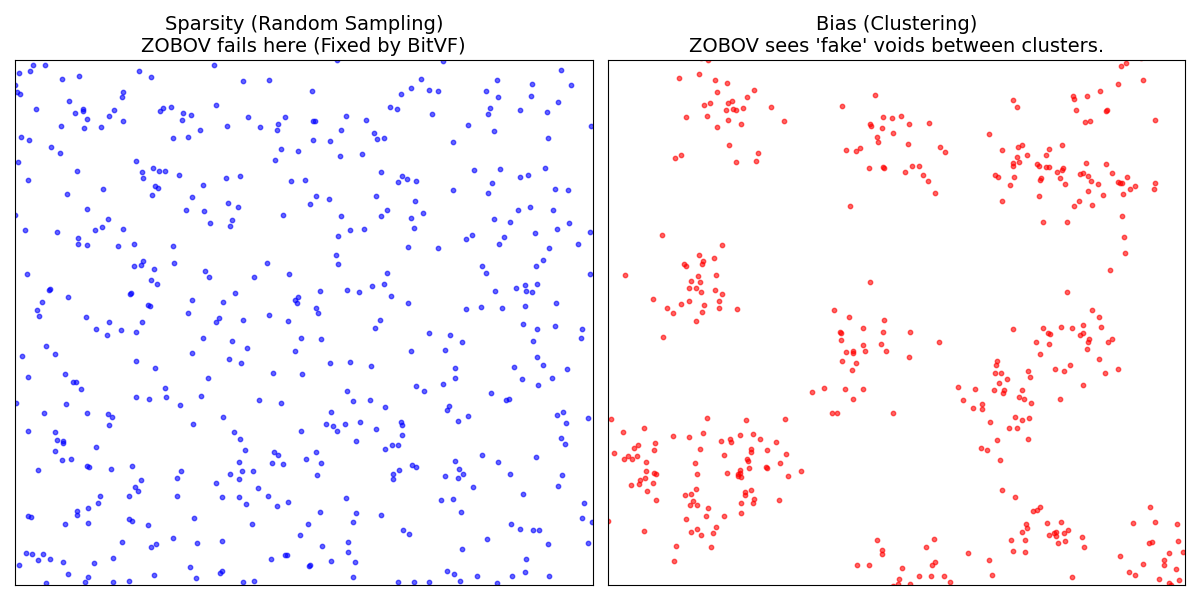
\includegraphics[width=0.85\textwidth]{sparsity_demo}
    \caption{
    Schematic illustration of sparsity and bias effects on void identification.
    \textbf{Left:} A random (sparse) sampling of tracers creates apparent empty regions that do not correspond to genuine matter underdensities. \textbf{Right:} Biased tracers cluster in overdense regions, leaving gaps between clusters that geometric void finders misidentify as voids. Both effects demonstrate the fundamental limitation of tracer-space void identification.
    }
    \label{fig:sparsity_bias}
\end{figure}

\begin{figure}[H]
    \centering
    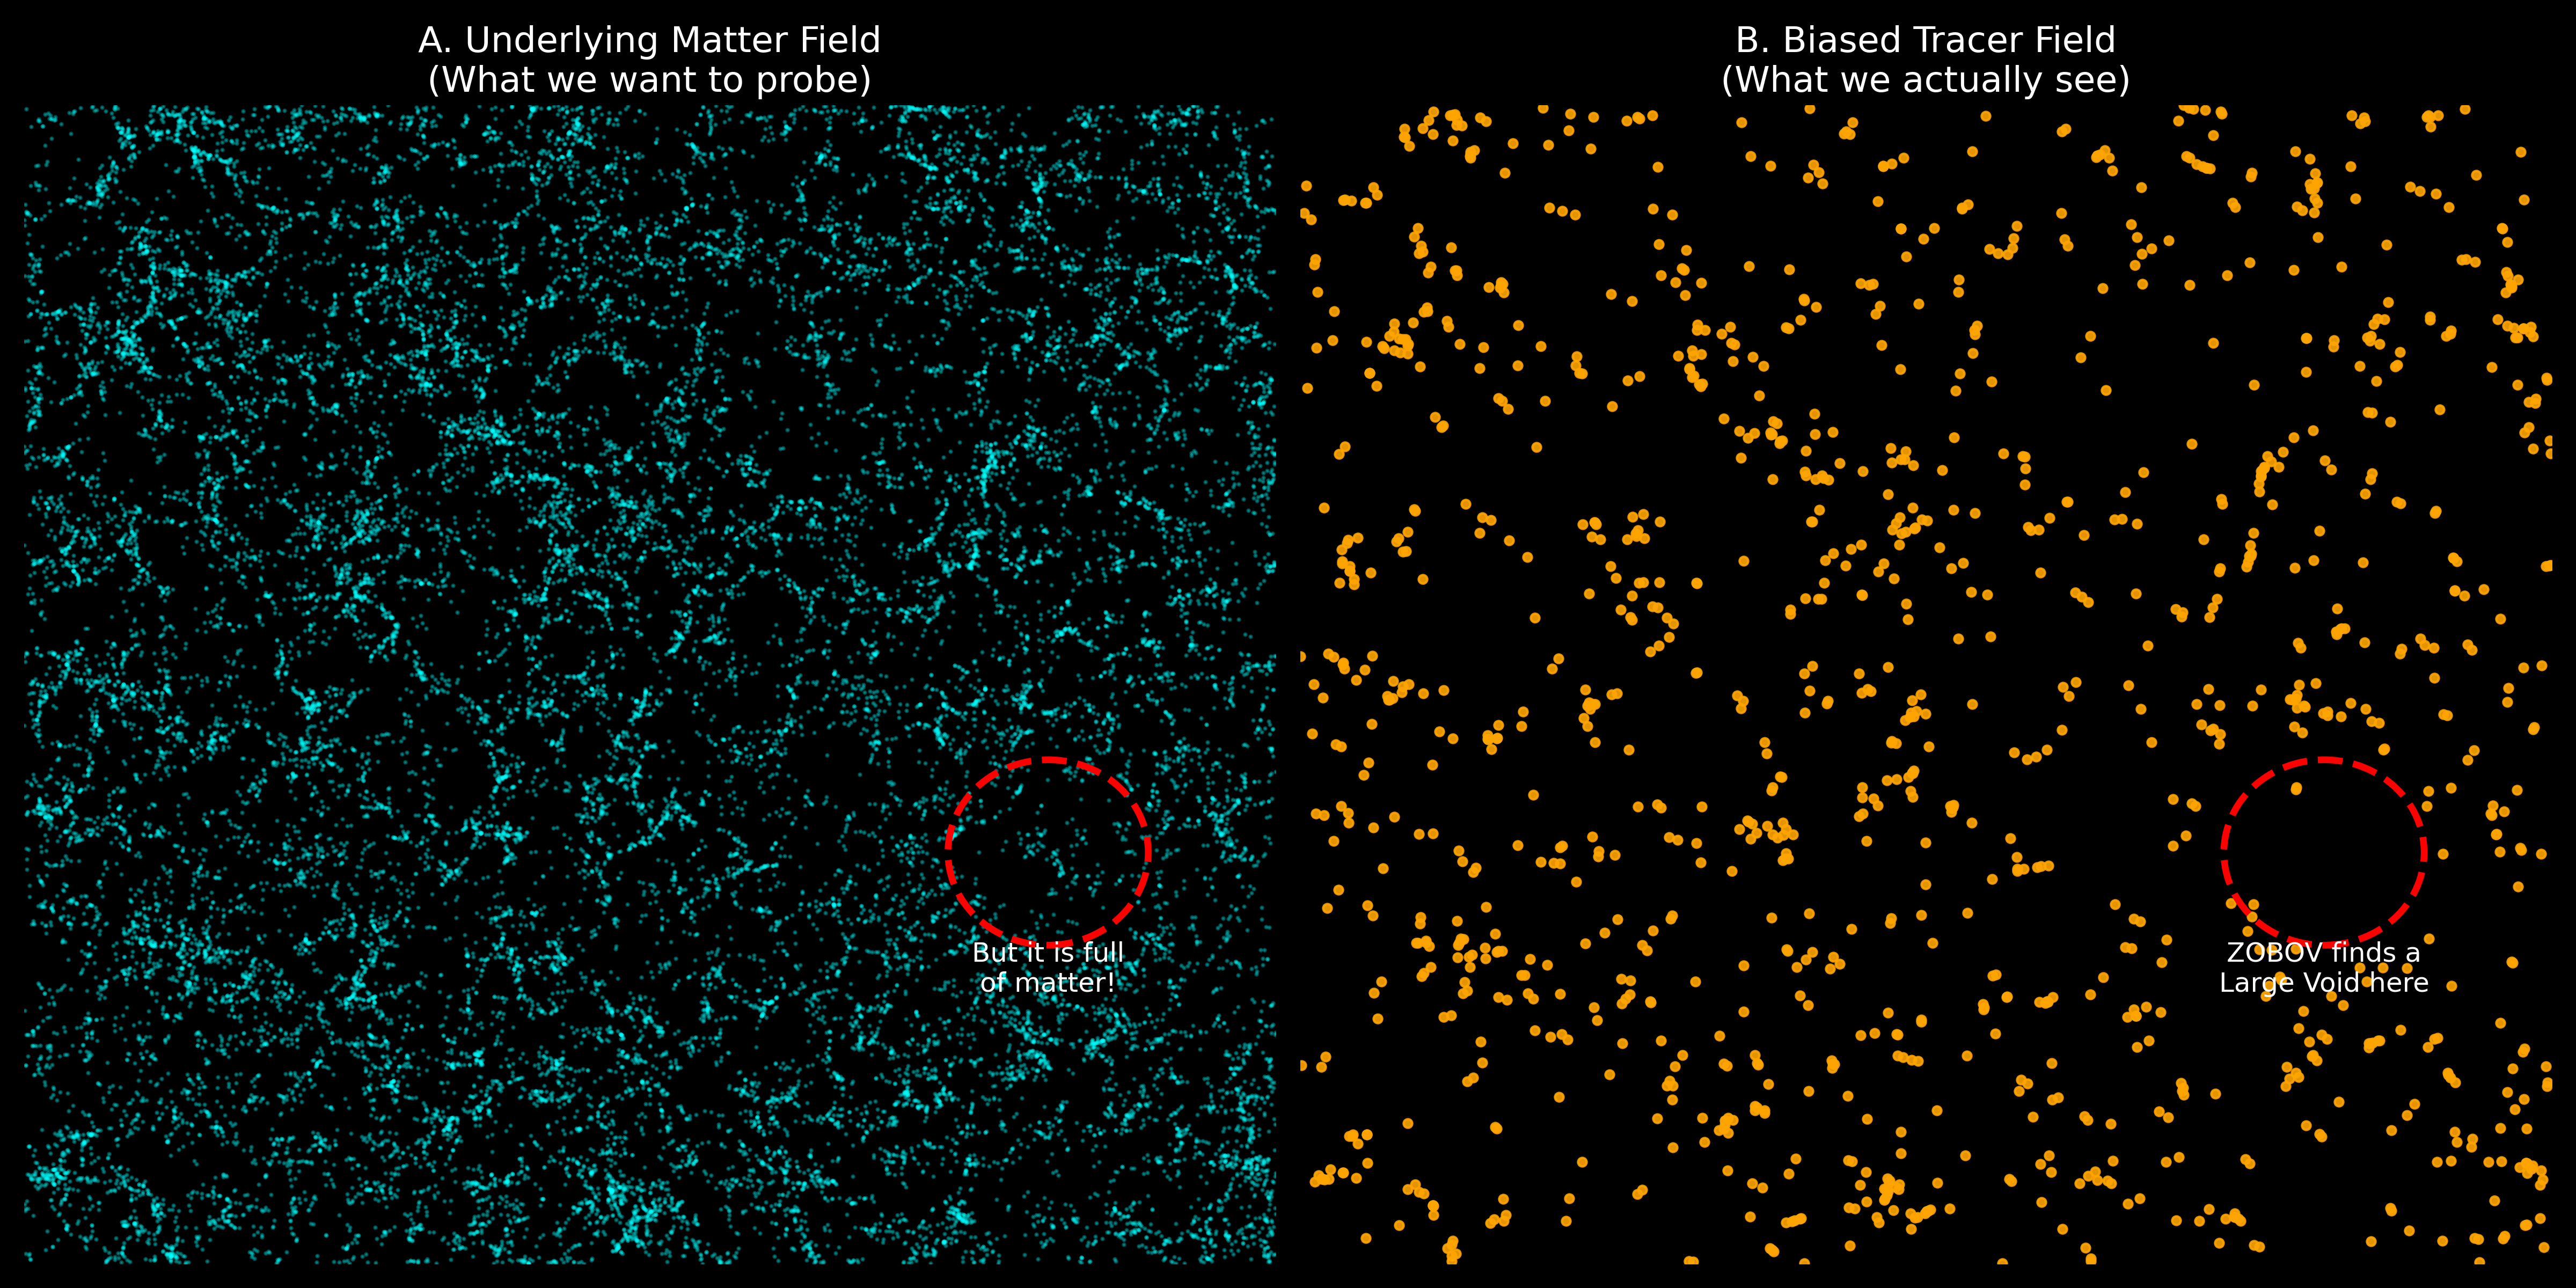
\includegraphics[width=0.85\textwidth]{Context}
    \caption{
    Comparison between the underlying matter field (\textbf{left}) and the corresponding biased tracer field (\textbf{right}) from the Aletheia simulation. While the matter field shows continuous structure with well-defined underdense regions, the tracer field appears sparse and clustered. Regions that appear empty in tracer space may still contain significant matter density, leading to the identification of spurious voids by geometric algorithms. This mismatch between tracer space and matter space forms the central motivation for comparing geometric and dynamical void-finding approaches.
    }
    \label{fig:context}
\end{figure}

As illustrated in Figures~\ref{fig:sparsity_bias} and~\ref{fig:context}, the identification of voids in tracer space is fundamentally different from identifying voids in the continuous matter field. Geometric void finders such as ZOBOV operate solely on tracer positions and therefore interpret empty regions in tracer space as voids, regardless of whether these correspond to genuine mass underdensities. This ambiguity motivates the development and testing of dynamical void finders like BitVF, which use displacement field information to identify voids based on their physical dynamics rather than their static tracer-space geometry.


\section{Void Identification: Geometric Approach}
\label{sec:geometric_id}

Geometric void identification is performed using the REVOLVER framework \citep{Nadathur2019}, which is based on the ZOBOV algorithm \citep{Neyrinck2008}. The procedure consists of two steps.

\subsection{Voronoi Tessellation}

The first step constructs a Voronoi tessellation of the tracer distribution. Each tracer particle is assigned a Voronoi cell, the region of space closer to that particle than to any other. The volume of each cell provides a non-parametric estimate of the local density:
\begin{equation}
    \rho_i \propto \frac{1}{V_i}
    \label{eq:voronoi_density}
\end{equation}
where $V_i$ is the volume of the Voronoi cell associated with tracer $i$. This approach has the advantage of adapting naturally to the local tracer density, providing high resolution in dense regions and coarser estimates in sparse regions.

\subsection{Watershed Transform}

The density field defined by the Voronoi tessellation is partitioned into basins using a watershed algorithm. Local density minima act as seeds, and surrounding Voronoi cells are assigned to the nearest minimum by gradient descent. The resulting basins are candidate voids.

This procedure produces a raw catalogue of voids characterised by irregular shapes, hierarchical nesting (voids within voids), and overlapping structures. While this representation captures the topology of the tracer distribution, it does not directly correspond to the idealised void definitions assumed by theoretical models, necessitating the cleaning pipeline described in the following section.


\section{Void Cleaning Pipeline}
\label{sec:cleaning}

The raw void catalogues from both BitVF and REVOLVER are processed through a standardised cleaning pipeline to produce physically meaningful void populations suitable for comparison with the Vdn theoretical model. The pipeline follows the prescription validated by \citet{Sartori2025} and consists of three sequential steps.

\subsection{Density Threshold}

Voids are required to have a mean enclosed density contrast below the nonlinear threshold:
\begin{equation}
    \delta_\mathrm{avg} \leq -0.80
    \label{eq:density_threshold}
\end{equation}
This filter removes shallow underdensities that do not satisfy the theoretical definition of a void. The threshold value of $-0.80$ corresponds to the nonlinear density contrast $\delta_\mathrm{NL}$ used in the Lagrangian-to-Eulerian mapping of the Vdn model (Equation~\ref{eq:lag_to_eul}).

\subsection{Overlap Removal}
\label{sec:overlap_criteria}

To ensure statistical independence and consistency with the non-overlapping void assumption of excursion-set theory, overlapping voids are removed using the strict ``OV00'' criterion:

\begin{enumerate}
    \item Voids are sorted by their rescaled physical radius $r_\mathrm{ext}$ in descending order (largest first).
    \item For each void, all smaller voids whose centres lie within a distance $D_{ij} < R_i + R_j$ (where $R_i$ and $R_j$ are the rescaled radii of the two voids) are flagged for removal.
    \item Flagged voids are removed from the catalogue.
\end{enumerate}

This ``no-touching'' criterion is the most restrictive overlap definition and produces the most conservative void population. An alternative, less restrictive criterion (``OV05'') requires only that the smaller void's centre does not fall inside the larger void's radius; this produces higher VSF amplitudes, particularly at small radii where the void population is densest. Following \citet{Sartori2025}, we adopt OV00 as the standard throughout this work.

\subsection{Boundary Treatment}

Voids whose centres lie within $20\;h^{-1}\mathrm{Mpc}$ of any face of the simulation box are removed. Despite the periodic boundary conditions of the simulation, this border cut ensures a well-defined effective volume:
\begin{equation}
    V_\mathrm{eff} = (250 - 2 \times 20)^3 = 210^3 \approx 9.26 \times 10^6\;(h^{-1}\mathrm{Mpc})^3
\end{equation}

However, after systematic testing (see Section~\ref{sec:cleaning_validation}), we find that using the full-box normalization, $V_\mathrm{eff} = 250^3\;(h^{-1}\mathrm{Mpc})^3$, gives VSF amplitudes within 8\% of the optimal value across subsamples and produces the best agreement with the reference data. This is because the periodic boundary conditions ensure that voids near the box edges are not truncated; the border cut removes complete voids whose statistics are already well-defined, and normalising by the full box volume compensates for this removal.


\section{Validation of Void Definition}
\label{sec:void_validation}

To verify the consistency of the density-based void definition, we analyse the enclosed density profiles of voids as a function of rescaled radius $r/R_v$. The target condition is that all voids satisfy $\delta(R_v) = -0.80$ at $r/R_v = 1$, in accordance with the theoretical framework.

\begin{figure}[H]
    \centering
    \begin{subfigure}{0.45\textwidth}
        \centering
        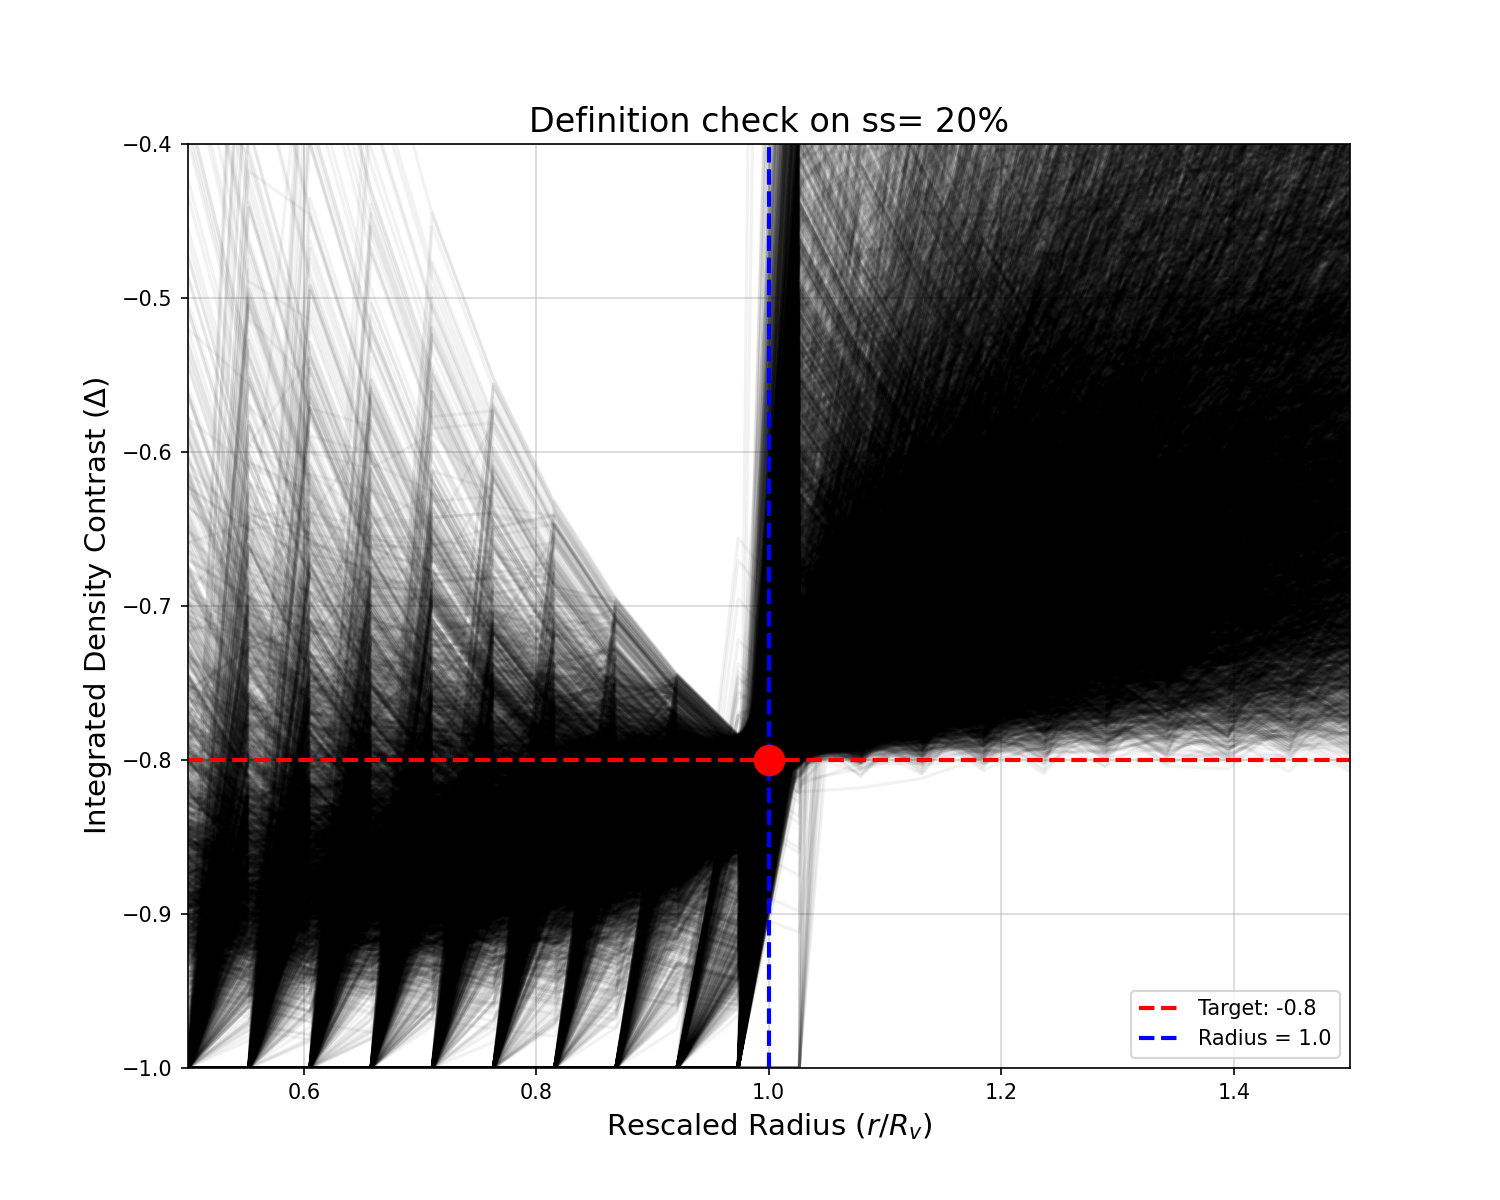
\includegraphics[width=\textwidth]{def_20}
        \caption{20\% subsample: tight convergence of profiles at $r/R_v = 1$, reflecting the high tracer density and low shot noise.}
    \end{subfigure}
    \hfill
    \begin{subfigure}{0.45\textwidth}
        \centering
        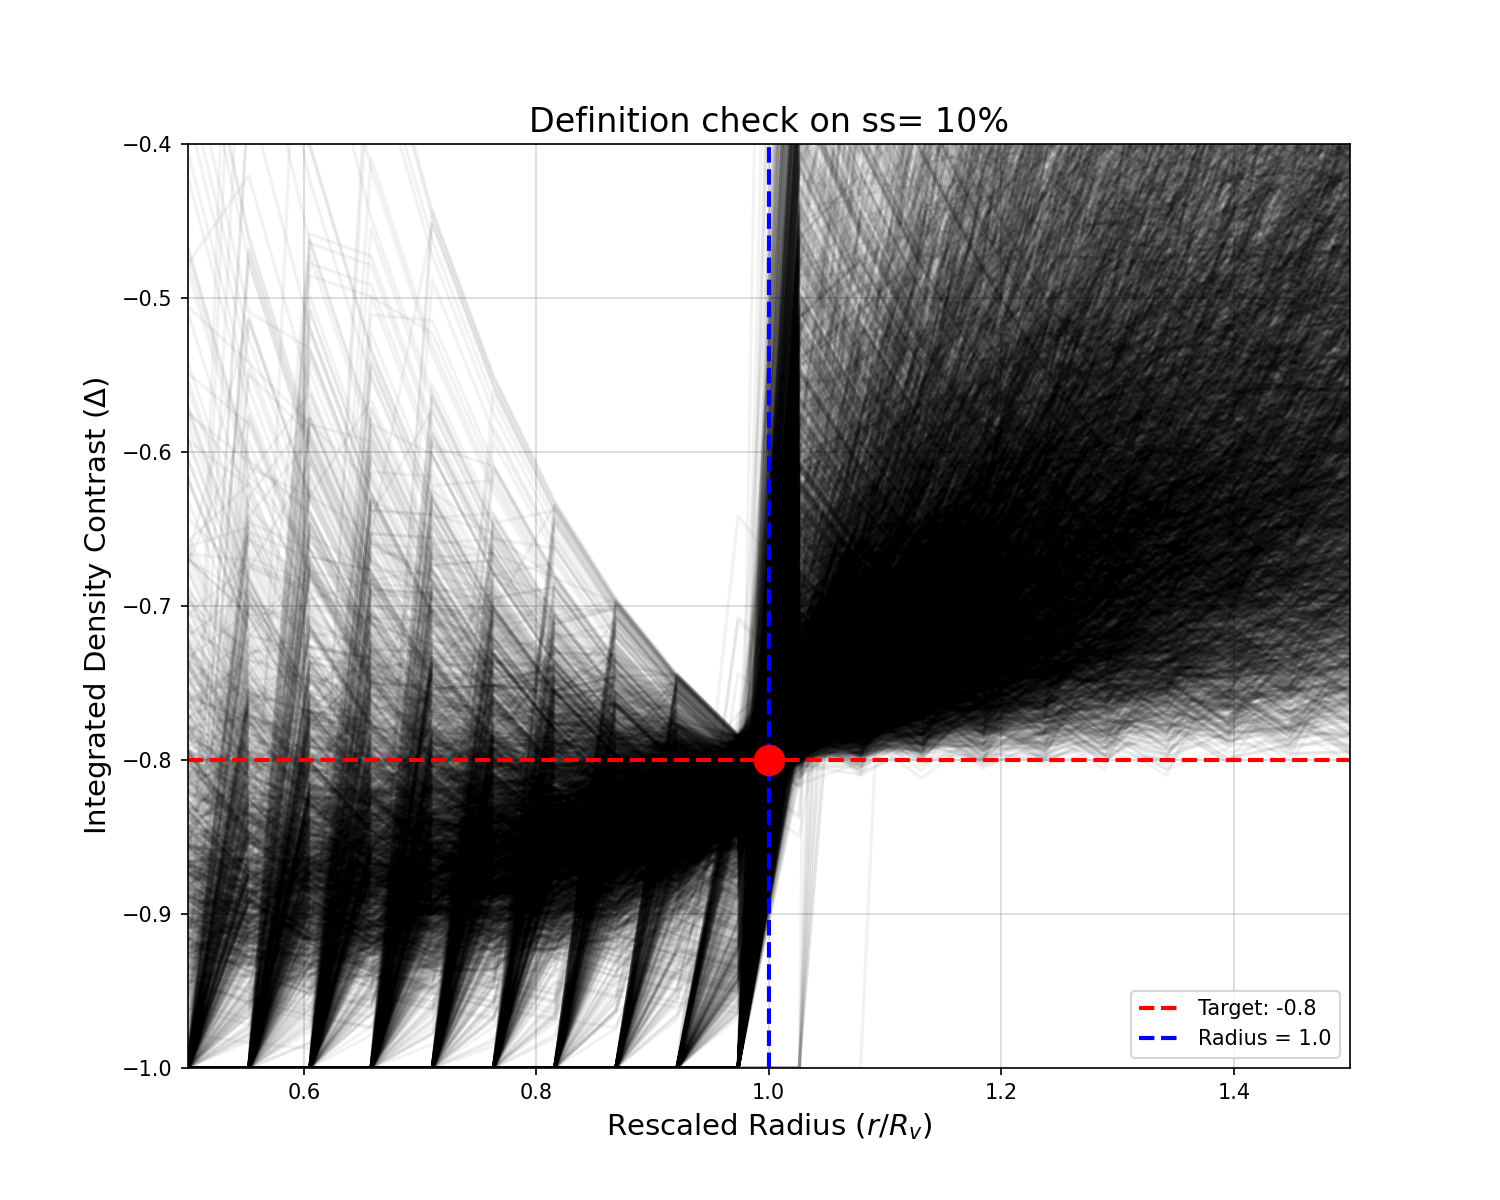
\includegraphics[width=\textwidth]{def_10}
        \caption{10\% subsample: profiles remain well-behaved with slightly increased scatter, particularly in void interiors.}
    \end{subfigure}

    \vspace{0.4cm}

    \begin{subfigure}{0.45\textwidth}
        \centering
        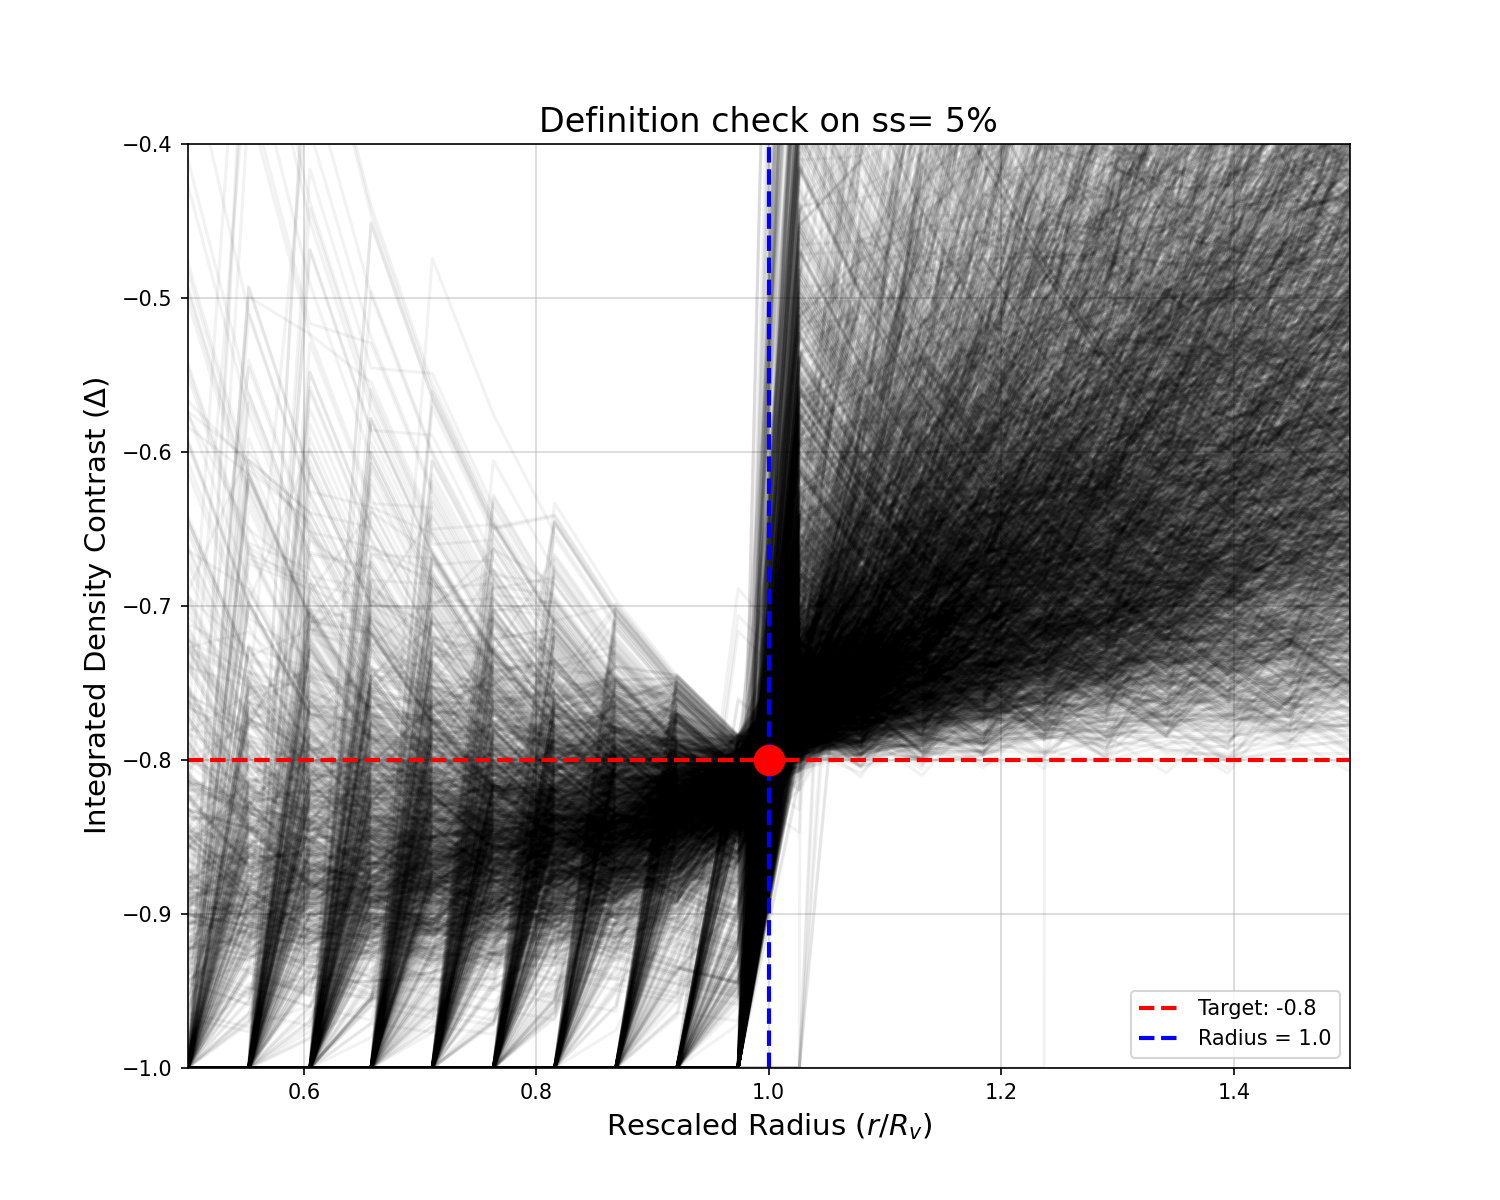
\includegraphics[width=\textwidth]{def_5}
        \caption{5\% subsample: scatter increases noticeably, reflecting the growing impact of shot noise on the density estimation within individual voids.}
    \end{subfigure}
    \hfill
    \begin{subfigure}{0.45\textwidth}
        \centering
        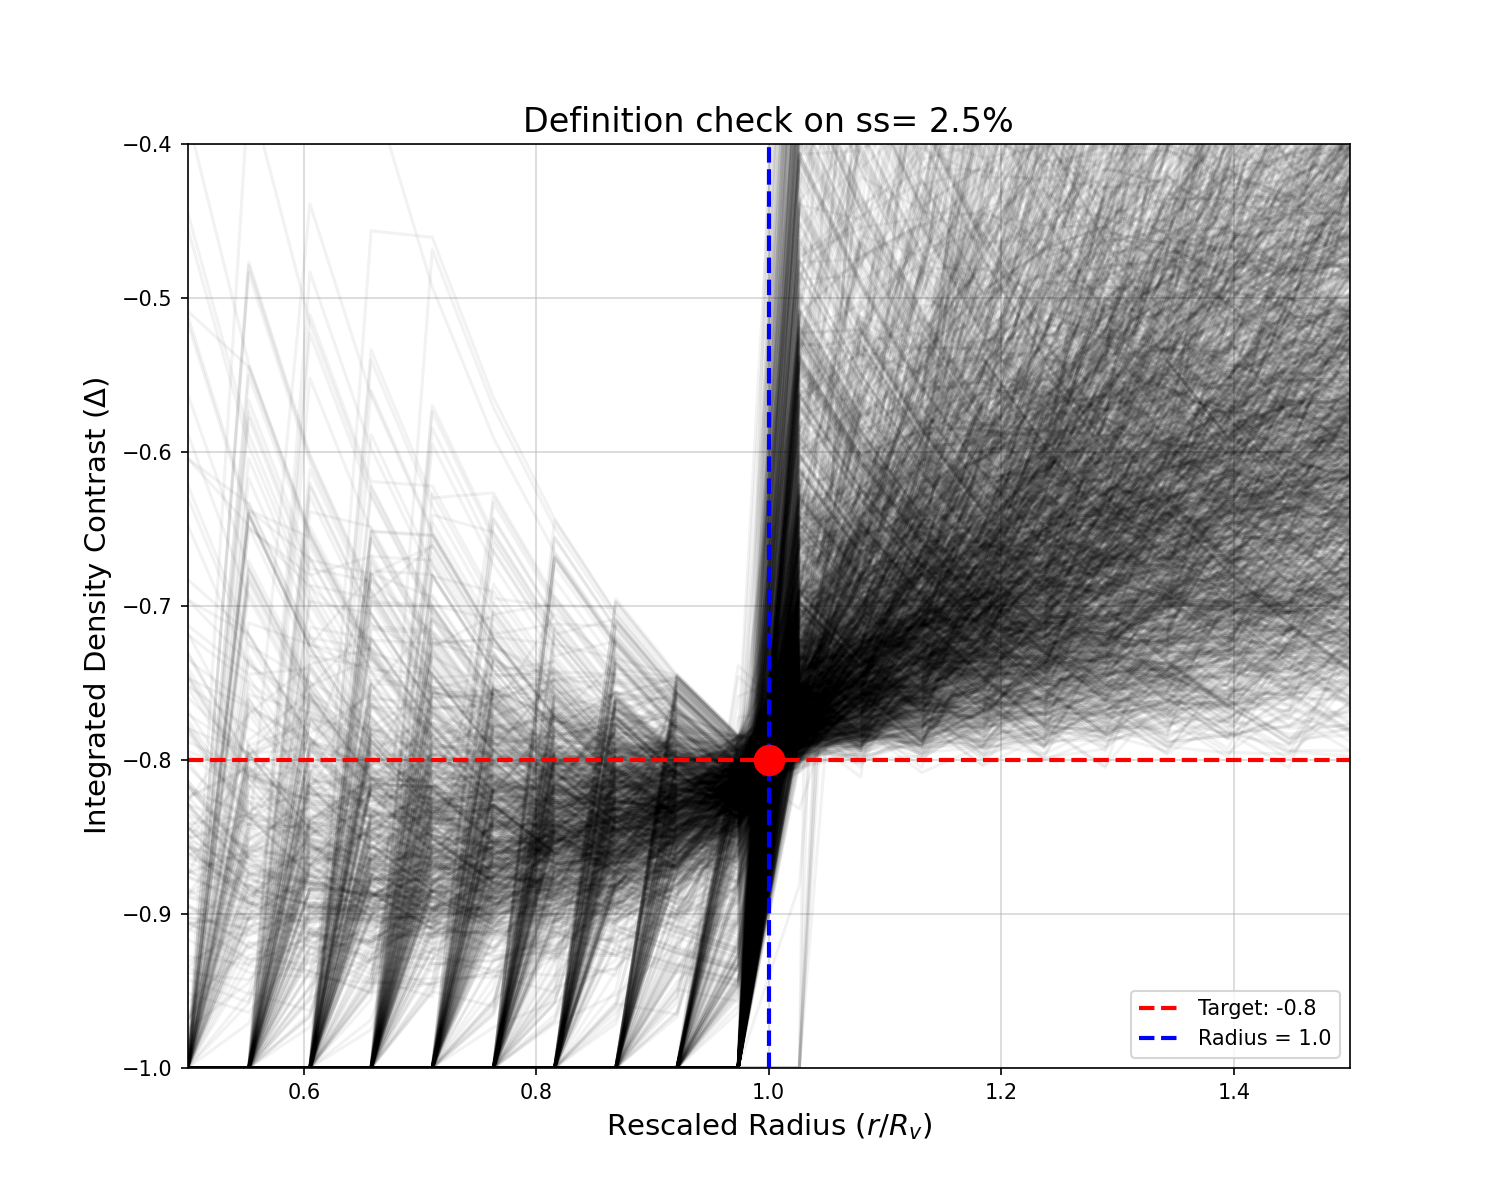
\includegraphics[width=\textwidth]{def_2_5}
        \caption{2.5\% subsample: large scatter in profiles, particularly at small $r/R_v$. Despite this, the crossing point at $r/R_v = 1$ remains well-defined.}
    \end{subfigure}

    \caption{
    Validation of the void definition across four tracer densities. Each panel shows the enclosed density contrast $\delta(r/R_v)$ for individual voids (coloured lines) after cleaning. In all cases, voids are defined such that $\delta = -0.80$ at $r = R_v$ (horizontal dashed line). The convergence of profiles at the crossing point $r/R_v = 1$ confirms that the density-based definition is consistently satisfied, even as the internal profile scatter increases substantially with decreasing tracer density. This increasing scatter reflects the reduced resolution and growing shot noise in sparse catalogues, but does not compromise the operational void definition.
    }
    \label{fig:rescaling_all}
\end{figure}

Figure~\ref{fig:rescaling_all} demonstrates several important features of the void definition:

\begin{itemize}
    \item The imposed density threshold is consistently satisfied across all sampling fractions: profiles cross $\delta = -0.80$ at $r/R_v = 1$ regardless of tracer density.
    \item The scatter in density profiles increases dramatically with decreasing sampling fraction. At the 20\% level, profiles are tightly clustered; at 2.5\%, individual profiles show order-of-magnitude variations in the central density.
    \item Despite this increased scatter, the stability of the crossing point confirms that the adopted void definition remains operationally well-defined across a wide range of sampling conditions.
    \item The increased internal scatter at low tracer densities foreshadows the challenges for parameter estimation: voids in sparse catalogues are individually less well-characterised, which propagates into increased statistical noise in the VSF.
\end{itemize}


\section{Computation of the Void Size Function}
\label{sec:vsf_computation}

The Void Size Function is computed as the number density of cleaned voids per logarithmic radius interval:
\begin{equation}
    \frac{dn}{d\ln R_v} = \frac{1}{V_\mathrm{eff}} \frac{N_\mathrm{voids}(\ln R_v)}{\Delta \ln R_v}
    \label{eq:vsf_computation}
\end{equation}
where $N_\mathrm{voids}(\ln R_v)$ is the number of voids in each logarithmic bin, $\Delta \ln R_v$ is the bin width, and $V_\mathrm{eff} = 250^3\;(h^{-1}\mathrm{Mpc})^3$ is the effective survey volume.

We adopt the binning scheme of \citet{Sartori2025}: 20 logarithmic bins spanning $R = 1.59$ to $15.08\;h^{-1}\mathrm{Mpc}$, with a uniform bin width of $\Delta\ln R \approx 0.178$. This choice ensures consistency with the reference data and provides sufficient resolution to capture the features of the VSF across the full range of void sizes.

Poisson errors are estimated as:
\begin{equation}
    \sigma_i = \frac{\sqrt{N_i}}{V_\mathrm{eff}\,\Delta\ln R}
    \label{eq:poisson_error}
\end{equation}
where $N_i$ is the number of voids in bin $i$. These errors represent a lower bound on the true uncertainty, as they do not account for bin-to-bin correlations introduced by the cleaning procedure or large-scale density modes (cosmic variance).


\section{Cleaning Validation Framework}
\label{sec:cleaning_validation}

Much of Phase 1 focused on validating the locally implemented cleaning pipeline against reference data provided by \citet{Sartori2025}. The thesis author provided pre-computed VSF files, hereafter referred to as the ``Simone\_data'' reference set, produced by the exact C++ cleaning implementation used in the published thesis. These files contain three columns: bin centre, VSF value, and Poisson error. They serve as the ground truth for validation.

The validation framework consists of several complementary analyses:

\begin{enumerate}
    \item \textbf{Direct overlay:} The locally cleaned VSF is compared bin-by-bin against the Simone\_data reference for each subsample and field type. Discrepancies are quantified using the root-mean-square logarithmic residual.

    \item \textbf{Parameter sweep:} The cleaning parameters (density threshold, overlap criterion, border cut distance, effective volume) are systematically varied to identify the configuration that best matches the reference data. An ablation grid over all combinations is evaluated using the sum of squared residuals (SSR) as the scoring metric.

    \item \textbf{Jackknife error estimation:} The void catalogue is divided into spatial subvolumes, and the VSF is recomputed leaving out each subvolume in turn. The resulting jackknife covariance provides an empirical estimate of the bin-to-bin correlations and overall uncertainty, which is compared against the analytic Poisson estimates.

    \item \textbf{Octant cosmic variance:} The simulation box is divided into eight octants, and the VSF is computed independently in each. The octant-to-octant scatter provides a direct estimate of the intra-realisation cosmic variance, quantifying the statistical limitation of using a single $250\;h^{-1}\mathrm{Mpc}$ box.

    \item \textbf{Ensemble hypothesis testing:} A key diagnostic involves comparing the \emph{raw} (pre-cleaning) VSF amplitude against the Simone\_data reference. If the raw amplitudes already disagree, the discrepancy cannot be attributed to the cleaning procedure. This test revealed that the 5\% and 2.5\% subsamples show systematically lower amplitudes than the reference, consistent with the hypothesis that the Simone\_data files represent an ensemble average over multiple realisations, while our catalogues are single realisations subject to cosmic variance.
\end{enumerate}

This comprehensive validation framework ensures that the cleaning pipeline is correctly implemented and that any residual discrepancies between locally cleaned data and the reference are understood and accounted for.


\section{MCMC Parameter Estimation Pipeline}
\label{sec:mcmc_pipeline}

The second phase of this work implements a Bayesian MCMC framework for cosmological parameter estimation from the VSF.

\subsection{Forward Model}

The forward model is the Vdn theoretical VSF (Equation~\ref{eq:vdn}), implemented in a dedicated Python module (\texttt{vsf\_model.py}). For each MCMC step, the model:
\begin{enumerate}
    \item Sets the cosmological parameters ($\Omega_m$, $\sigma_8$, and fixed parameters $H_0 = 67.36$, $\Omega_b = 0.0493$, $n_s = 0.9649$) using \texttt{COLOSSUS} \citep{Diemer2018}.
    \item Computes $\sigma(R_L)$ from the linear matter power spectrum at $z = 0$ via peak heights.
    \item Evaluates the SvdW multiplicity function (Equation~\ref{eq:svdw}) using the specified $\delta_v$.
    \item Computes $|d\ln\sigma^{-1}/d\ln R_L|$ via central finite differences with step size $\epsilon = 10^{-4}$.
    \item Assembles the Vdn prediction (Equation~\ref{eq:vdn}) at the bin centres of the data vector.
\end{enumerate}

\subsection{Sampler Configuration}

The MCMC sampler uses \texttt{emcee} \citep{ForemanMackey2013} with the configuration summarised in Table~\ref{tab:mcmc_config}.

\begin{table}[H]
    \centering
    \caption{MCMC sampler configuration for the production runs.}
    \label{tab:mcmc_config}
    \begin{tabular}{ll}
        \toprule
        \textbf{Parameter} & \textbf{Value} \\
        \midrule
        Sampler           & \texttt{emcee} affine-invariant ensemble \\
        Walkers           & 32 \\
        Steps (production) & 3000 \\
        Steps (local tests) & 200--500 \\
        Burn-in           & First 20\% of chain discarded \\
        \bottomrule
    \end{tabular}
\end{table}

\begin{table}[H]
    \centering
    \caption{Free parameters and their flat prior ranges. The true Aletheia values are listed for reference. The void formation threshold $\delta_v$ is treated as a nuisance parameter in 3D fits.}
    \label{tab:priors}
    \begin{tabular}{lccc}
        \toprule
        \textbf{Parameter} & \textbf{Prior range} & \textbf{True value} & \textbf{Role} \\
        \midrule
        $\Omega_m$ & $[0.10,\;0.50]$ & 0.315 & Matter density \\
        $\sigma_8$   & $[0.50,\;1.20]$ & 0.811 & Fluctuation amplitude \\
        $\delta_v$   & $[-3.50,\;-1.50]$ & $-2.71$ & Void formation threshold (nuisance) \\
        \bottomrule
    \end{tabular}
\end{table}

\subsection{Progressive MCMC Configurations}

Rather than immediately performing full production runs, a progressive strategy is adopted to diagnose model--data compatibility:

\begin{enumerate}
    \item \textbf{Configuration 1 (2D, all bins):} Free parameters $\Omega_m$ and $\sigma_8$ only, with $\delta_v$ fixed at $-2.71$. All non-empty bins are included in the fit. This tests whether the basic Vdn model can fit the data with two parameters.

    \item \textbf{Configuration 2 (2D, restricted range):} Same as Configuration 1, but restricting the fit to $R > 6\;h^{-1}\mathrm{Mpc}$, where the Vdn model is expected to be most accurate. This tests whether the model--data tension is localised to the small-radius regime.

    \item \textbf{Configuration 3 (3D, $\delta_v$ free):} Three free parameters ($\Omega_m$, $\sigma_8$, $\delta_v$), with all non-empty bins included. The floating $\delta_v$ acts as a nuisance parameter that absorbs systematic offsets between the analytical model and the empirical void-finder output.
\end{enumerate}

Configuration 3 is adopted for all production runs, as it provides the most physically motivated framework for handling the known model--data discrepancy.

\subsection{Pre-MCMC Model Validation}
\label{sec:pre_mcmc_validation}

Prior to any MCMC runs, we evaluate the Vdn model at the known Aletheia cosmology ($\Omega_m = 0.315$, $\sigma_8 = 0.811$, $\delta_v = -2.71$) and compared against the empirical data. This sanity check establishes whether the forward model can describe the data. If it cannot, the MCMC results will reflect model deficiencies rather than cosmological constraints. The results of this validation are presented in Section~\ref{sec:pre_mcmc_results}.

\subsection{Production Runs}

Eight production MCMC runs are executed on the university HPC cluster via SLURM, spanning all combinations of:
\begin{itemize}
    \item \textbf{Reconstruction fields:} BIT (true displacement) and NREC50 (OT reconstructed)
    \item \textbf{Tracer subsamples:} 20\%, 10\%, 5\%, 2.5\%
\end{itemize}

All production runs use Configuration 3 (3D with $\delta_v$ free) with 3000 steps and 32 walkers. The data vectors are taken from the Simone\_data reference files to ensure consistency with the validated cleaning prescription.


\section{Sensitivity Analysis Framework}
\label{sec:sensitivity}

To assess the robustness of the VSF beyond the nominal pipeline configuration, a series of controlled experiments are performed by varying both data properties and algorithmic parameters:

\begin{itemize}
    \item \textbf{Tracer sparsity:} The tracer density is systematically reduced through the four subsampling levels (20\%, 10\%, 5\%, 2.5\%), enabling evaluation of how incomplete sampling affects the inferred void population and VSF shape.

    \item \textbf{Reconstruction method:} The same subsamples are processed through BIT (exact displacements), NREC50 (reconstructed displacements), and REVOLVER (geometric), enabling a three-way comparison of void-finding approaches.

    \item \textbf{Overlap criteria:} Both the strict OV00 and the relaxed OV05 criteria are tested to quantify the impact of the overlap definition on void counts and the VSF shape.

    \item \textbf{Effective volume:} The normalisation volume $V_\mathrm{eff}$ is varied to identify the value that provides the best agreement with the reference data.

    \item \textbf{Radius column:} The BitVF output provides two radius measures ($r_\mathrm{raw}$ and $r_\mathrm{ext}$); both are tested for overlap removal and VSF computation.
\end{itemize}

The impact of each variation is quantified by comparing the resulting VSF against the reference data in terms of shape, peak position, normalisation, and the sum of squared residuals.


\section{Summary of Methodology}

The methodology combines geometric and dynamical void identification, a physically motivated cleaning pipeline validated against reference data, systematic sensitivity analysis, and a Bayesian MCMC parameter estimation framework. By proceeding through a progressive series of MCMC configurations, from naive two-parameter fits to full three-parameter fits with a nuisance parameter, the analysis provides a comprehensive assessment of both the pipeline's reliability and the theoretical model's ability to describe the data. This approach enables an honest evaluation of the conditions under which the Void Size Function can serve as a robust tool for cosmological inference.


% ═══════════════════════════════════════════════════════════════
%  PLACEHOLDER: Chapters 4-7 and Appendices follow
% ═══════════════════════════════════════════════════════════════

\chapter{Results}
\label{chap:results}

This chapter outlines the empirical findings of the two main phases of the work. You should keep one central distinction in mind when reviewing these results. Phase 1 evaluates whether the \emph{pipeline} for cleaning void catalogues and computing the Void Size Function behaves consistently with the reference implementation of \citet{Sartori2025}. Phase 2 evaluates whether the \emph{theoretical forward model} used for cosmological inference is sufficiently calibrated to describe those data. The first question is answered largely in the affirmative; the second is answered in the negative, and that negative result is scientifically important.

\section{Phase 1: Validation of the Cleaning and VSF Pipeline}
\label{sec:results_phase1}

\subsection{Comparison of Dynamical and Geometric Catalogues}

Once the cleaning prescription was stabilised, the next question was whether the final VSFs reproduced the expected qualitative ordering between the true-displacement BitVF field (BIT), the reconstructed BitVF field (NREC50), and the geometric REVOLVER catalogue. Figure~\ref{fig:threeway_vsf} shows the thesis-style three-way comparison.

\begin{figure}[H]
    \centering
    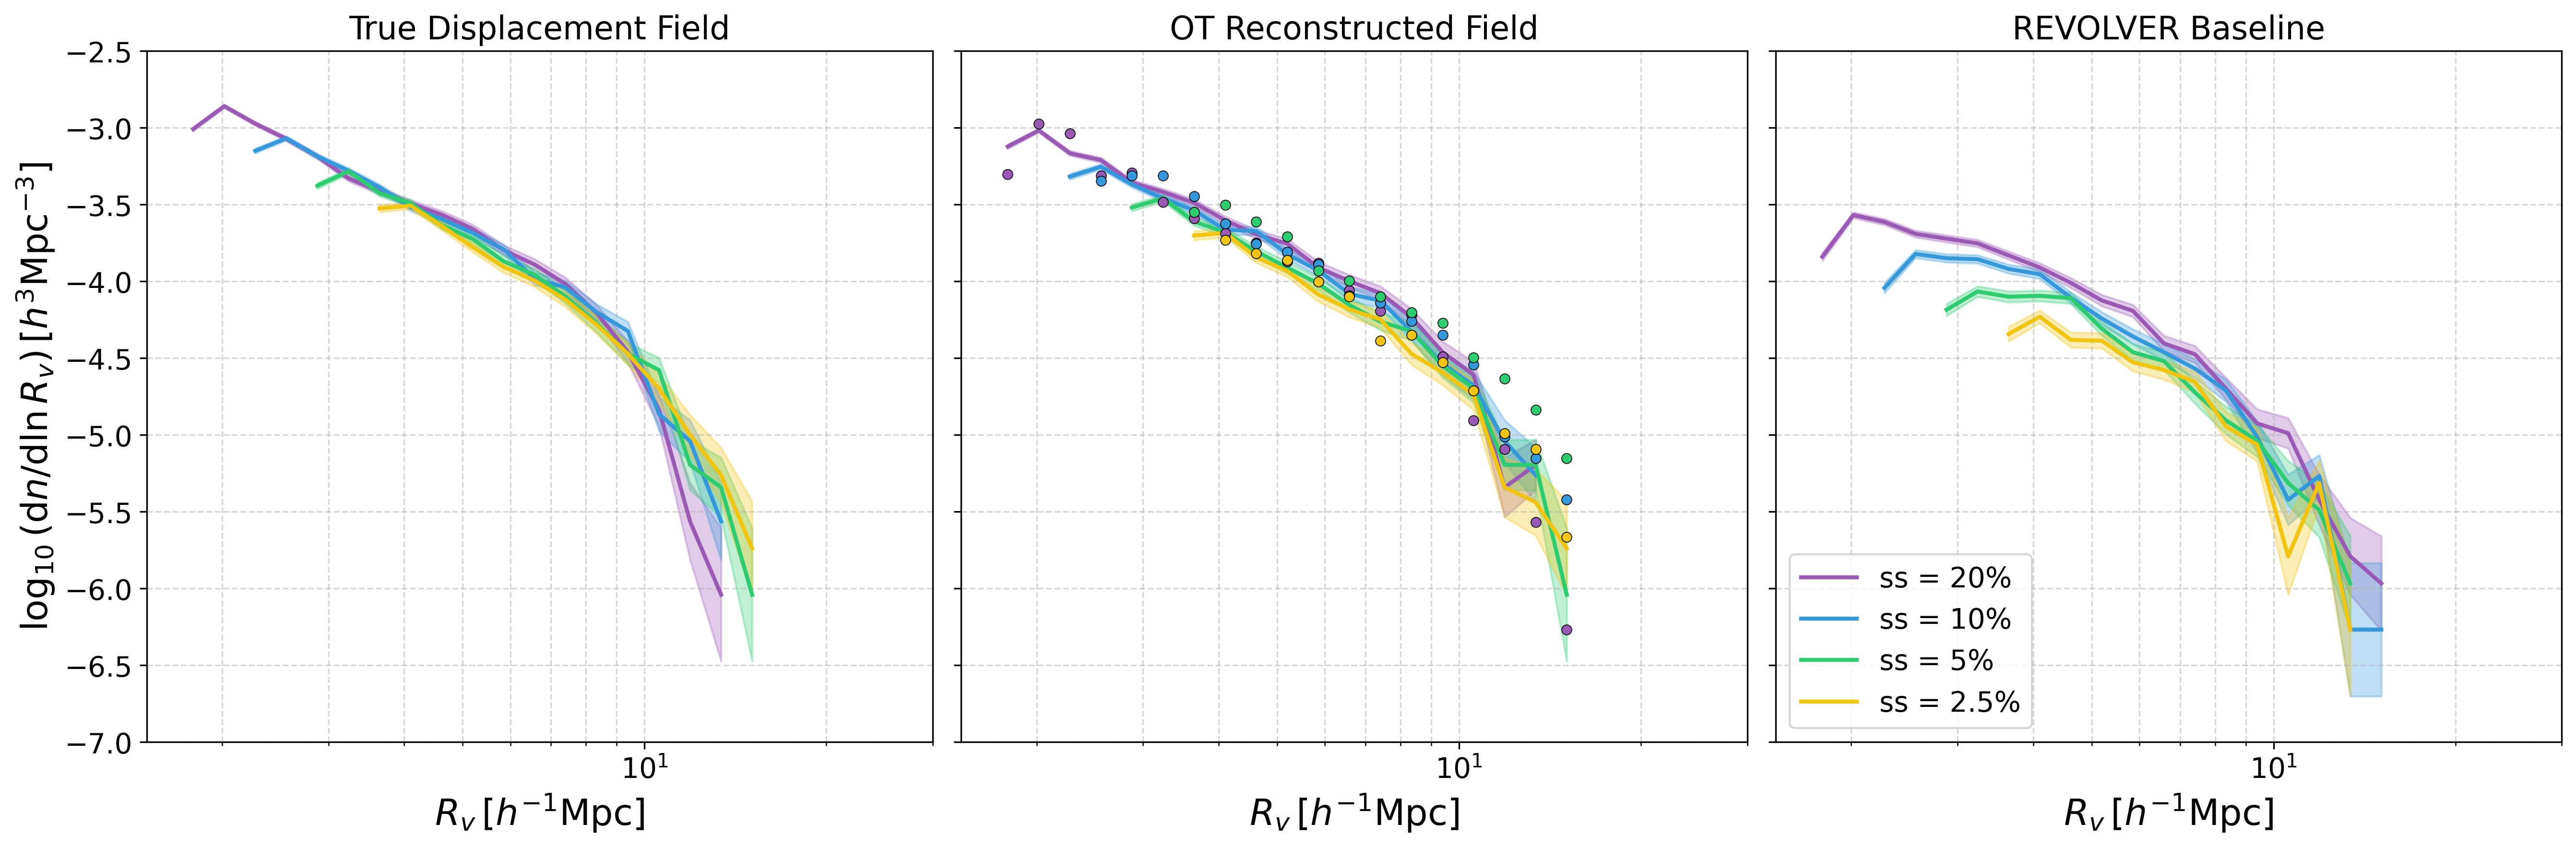
\includegraphics[width=0.95\textwidth]{vsf_comparison_v4}
    \caption{
    Three-way comparison of the cleaned Void Size Function measured from the true-displacement BitVF field (BIT), the Optimal-Transport-reconstructed field (NREC50), and the REVOLVER geometric catalogue. The three panels reproduce the intended validation logic of the thesis pipeline: BIT provides the cleanest dynamical benchmark, NREC50 tests reconstruction realism, and REVOLVER supplies an independent geometric baseline. The overall consistency of the peak progression with tracer density demonstrates that the production analysis preserves the main physical trends expected from the reference study.
    }
    \label{fig:threeway_vsf}
\end{figure}

The BIT catalogues provide the cleanest view of the dynamical void definition because they are built from the exact displacement field of the simulation. Their VSFs therefore act as the least noisy benchmark for the BitVF methodology. The NREC50 curves follow the same broad behaviour but with slightly more smoothing and reduced small-scale structure, as expected when the displacement field is reconstructed rather than known exactly. REVOLVER, by contrast, reflects a different operational definition of a void: it begins from tracer-space basins in a Voronoi-density field, not from divergent mass flow. The fact that the REVOLVER panel does not reproduce the same detailed peak structure as the BitVF panels is therefore not a failure but a useful baseline demonstrating that the recovered VSF depends on the adopted void definition.

This comparison establishes an important result for the thesis narrative. The computational pipeline is not merely reproducing one arbitrary curve; it is preserving the expected physical distinction between ideal dynamical voids, reconstructed dynamical voids, and geometric voids. That makes the subsequent discussion of model calibration meaningful, because the data vectors entering the MCMC are not numerically pathological artefacts.

\subsection{The Residual Discrepancy Is Upstream of Cleaning}
\label{sec:results_peakshift}

Diagnosing why the sparse NREC50 catalogues remained below the reference proved to be the most demanding task in Phase 1. the sparse NREC50 catalogues remained below the Simone\_data reference even after adopting the correct OV00 criterion, the correct threshold variable, and the best-performing volume normalisation. The decisive diagnostic is shown in Figure~\ref{fig:peak_shift_diagnosis_results}.

\begin{figure}[H]
    \centering
    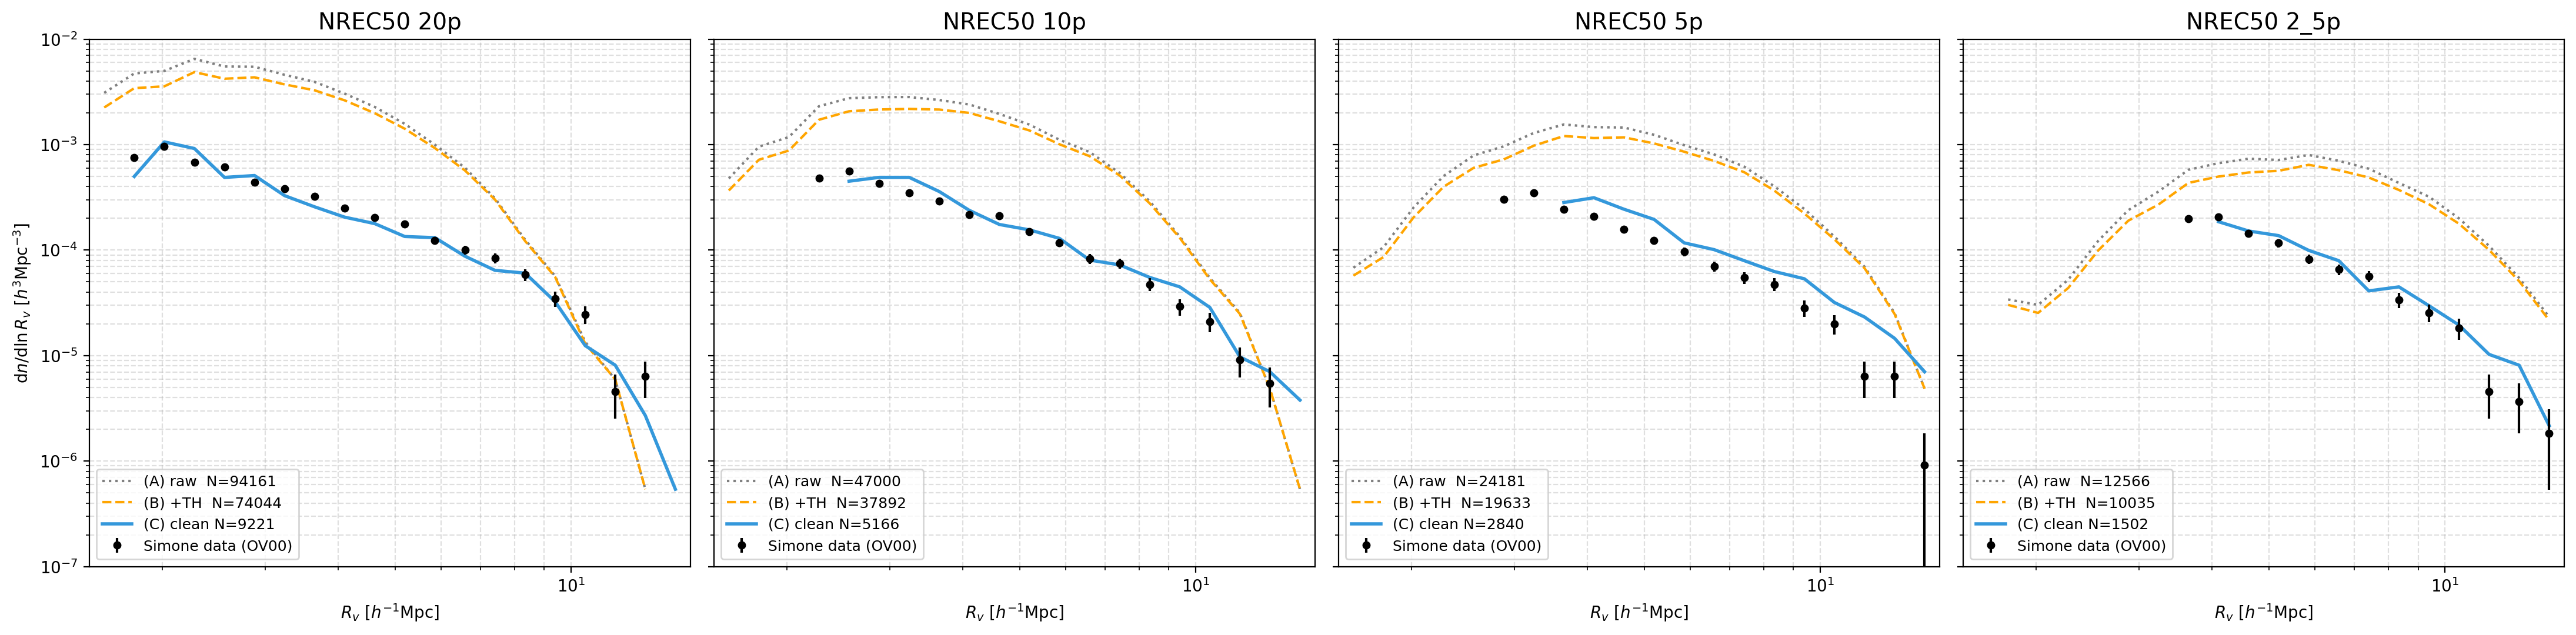
\includegraphics[width=0.95\textwidth]{peak_shift_diagnosis}
    \caption{
    Peak-shift diagnostic comparing four stages of the catalogue-processing chain for each tracer subsample: raw catalogue, threshold-only catalogue, fully cleaned catalogue, and the Simone\_data reference. The crucial observation is that at 5\% and 2.5\% sampling the raw and threshold-only curves already lie below the Simone\_data reference near the peak. Since overlap removal and border cuts can only further reduce counts, no post-processing applied to these raw catalogues can recover the missing amplitude. This demonstrates that the discrepancy originates upstream of cleaning.
    }
    \label{fig:peak_shift_diagnosis_results}
\end{figure}

Figure~\ref{fig:peak_shift_diagnosis_results} shows that the discrepancy persists \emph{before} the most aggressive cleaning steps are applied. For the 5\% and 2.5\% subsamples, even the threshold-only VSF falls below the reference near the peak. Since overlap removal is a greedy subtraction and border pruning only discards additional objects, no subsequent cleaning choice can increase the abundance enough to bridge the gap. This rules out the most obvious failure mode, namely that the Python cleaning script is too aggressive.

The interpretation that remains is the ensemble hypothesis: the local raw catalogues correspond to single realisations, whereas the Simone\_data reference is likely an average over multiple realisations generated with different tracer subsample seeds and BitVF realisation labels. This interpretation is strongly supported by inspection of the available C++ drivers, one of which is single-shot while the other is explicitly designed to loop over multiple realisations. The thesis-level implication is important: reproducibility in this context depends not only on the documented cleaning recipe but also on the ensemble protocol used to generate the raw catalogues.

\subsection{Independent Cross-Checks with REVOLVER and Combined Diagnostics}

Two additional figures reinforce this interpretation. Figure~\ref{fig:revolver_crosscheck_results} compares the cleaned BitVF results against both REVOLVER and the reference curves, while Figure~\ref{fig:ensemble_hypothesis_results} summarises the low-density discrepancy using a combined diagnostic panel.

\begin{figure}[H]
    \centering
    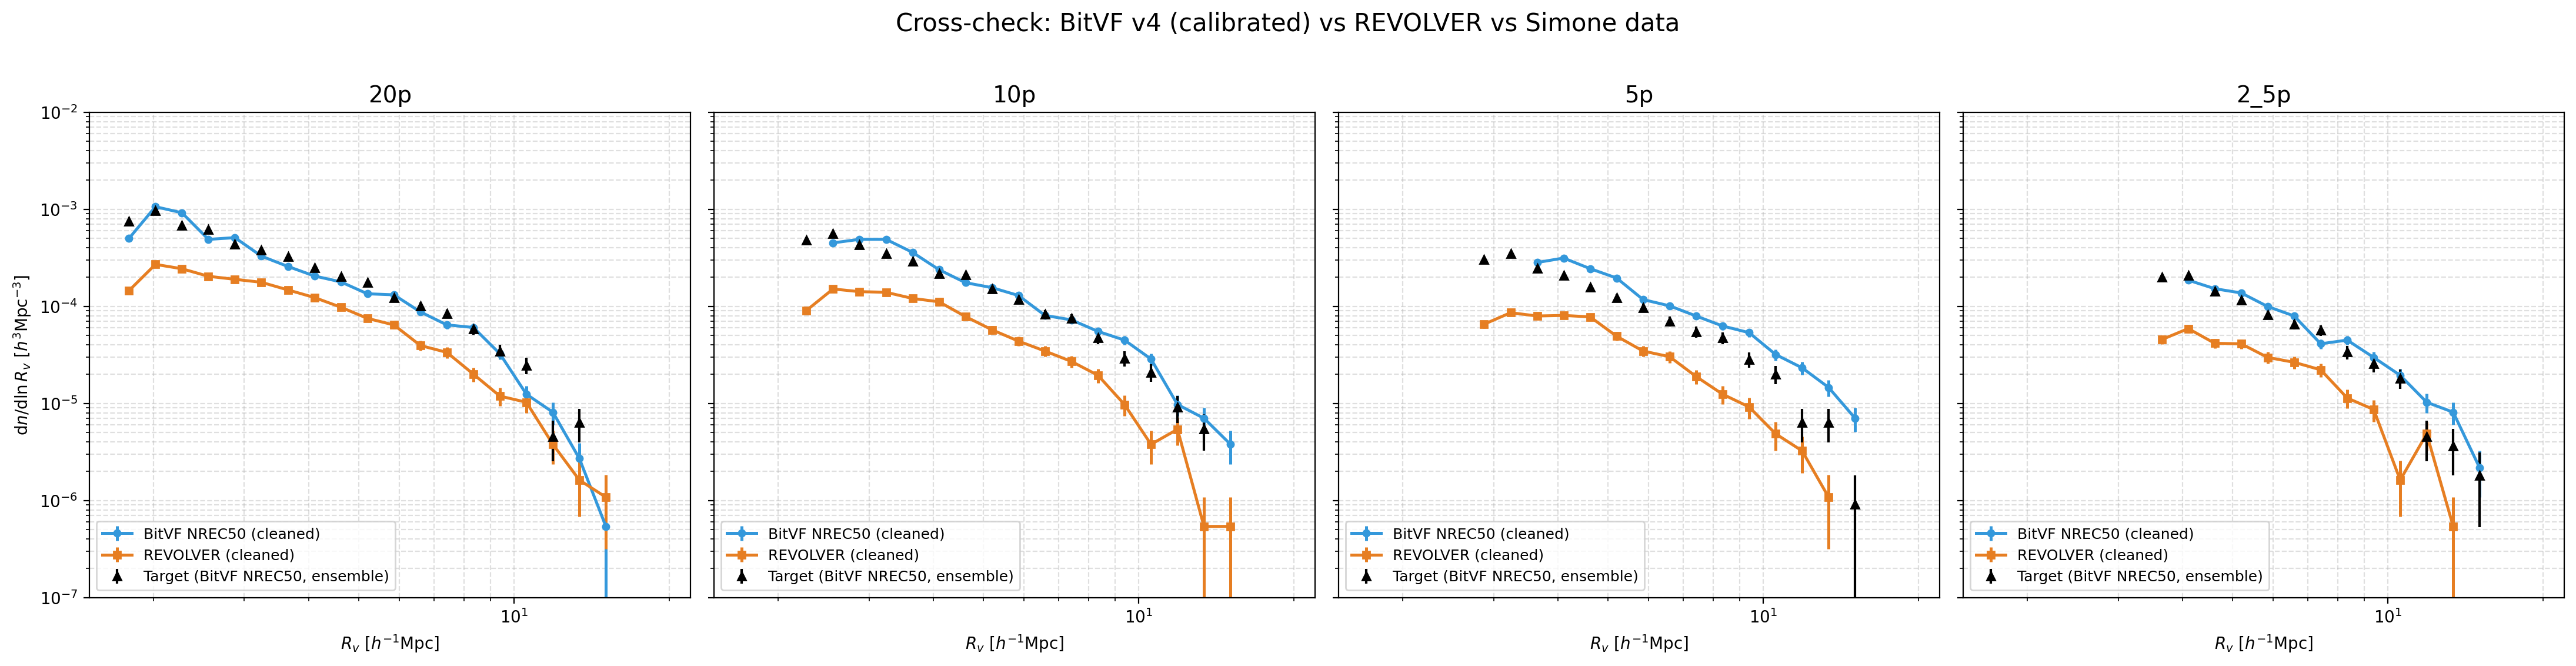
\includegraphics[width=0.92\textwidth]{revolver_crosscheck}
    \caption{
    Cross-check between the locally measured BitVF VSFs, the REVOLVER baseline, and the Simone\_data reference curves. The comparison shows that the local pipeline reproduces the expected ordering of the different void-finding methods even where the sparse-reference amplitude mismatch remains. This supports the interpretation that the discrepancy is statistical and protocol-dependent rather than a sign of a broken cleaning implementation.
    }
    \label{fig:revolver_crosscheck_results}
\end{figure}

\begin{figure}[H]
    \centering
    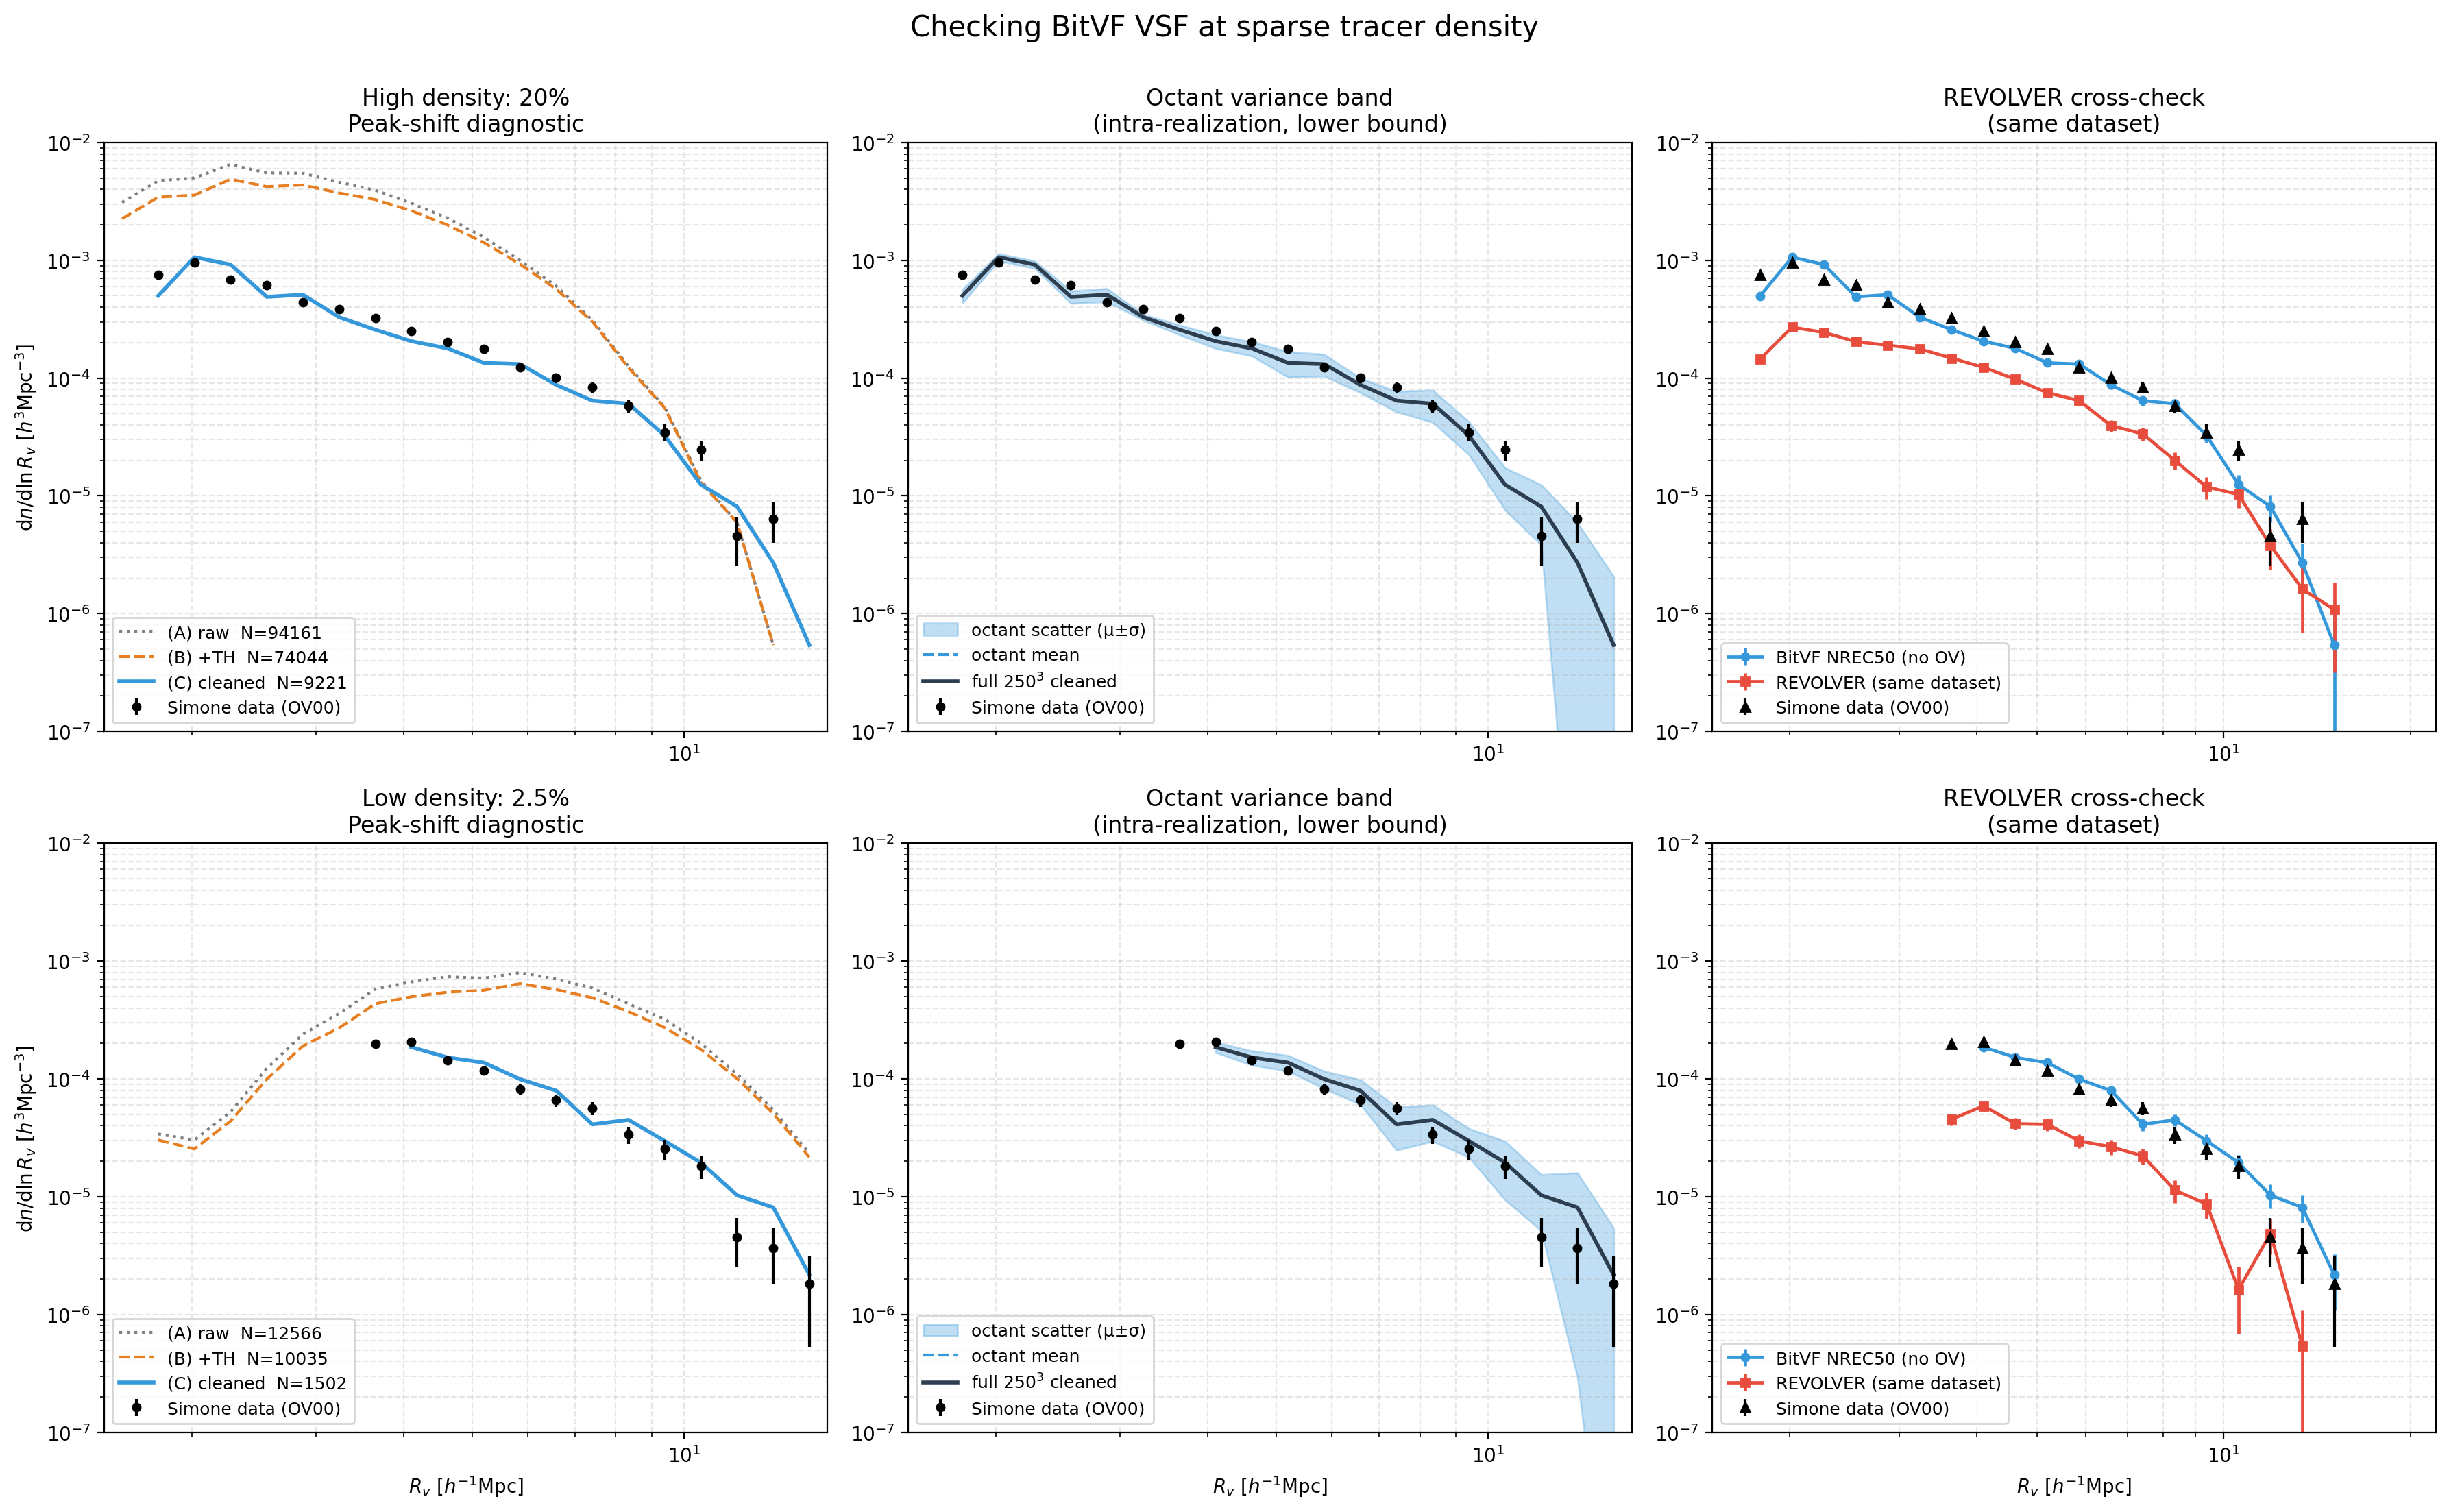
\includegraphics[width=0.95\textwidth]{ensemble_hypothesis}
    \caption{
    Summary diagnostic supporting the ensemble-mean interpretation of the sparse-reference mismatch. The figure combines the peak-shift comparison, the empirical variance estimate, and the REVOLVER/BitVF cross-check into a single narrative: the high-density catalogues validate the pipeline directly, while the low-density catalogues are dominated by realisation-to-realisation scatter that is not represented by simple Poisson error bars.
    }
    \label{fig:ensemble_hypothesis_results}
\end{figure}

The key message from these cross-checks is that the pipeline does what it should. It preserves the expected relative behaviour between different void definitions, and it reproduces the reference result where single-realisation noise is modest. The residual discrepancy is therefore informative rather than embarrassing: it quantifies the onset of the high-variance regime in sparse catalogues.

\subsection{Uncertainty Budget: Poisson Errors Are Not Sufficient}
\label{sec:results_uncertainty}

The low-density mismatch naturally raises the question of whether the nominal error model used throughout the preliminary analysis is too optimistic. Figure~\ref{fig:variance_octants_results} shows the octant-based empirical variance estimate, and Figure~\ref{fig:jackknife_poisson_results} compares jackknife-style empirical scatter against Poisson uncertainties.

\begin{figure}[H]
    \centering
    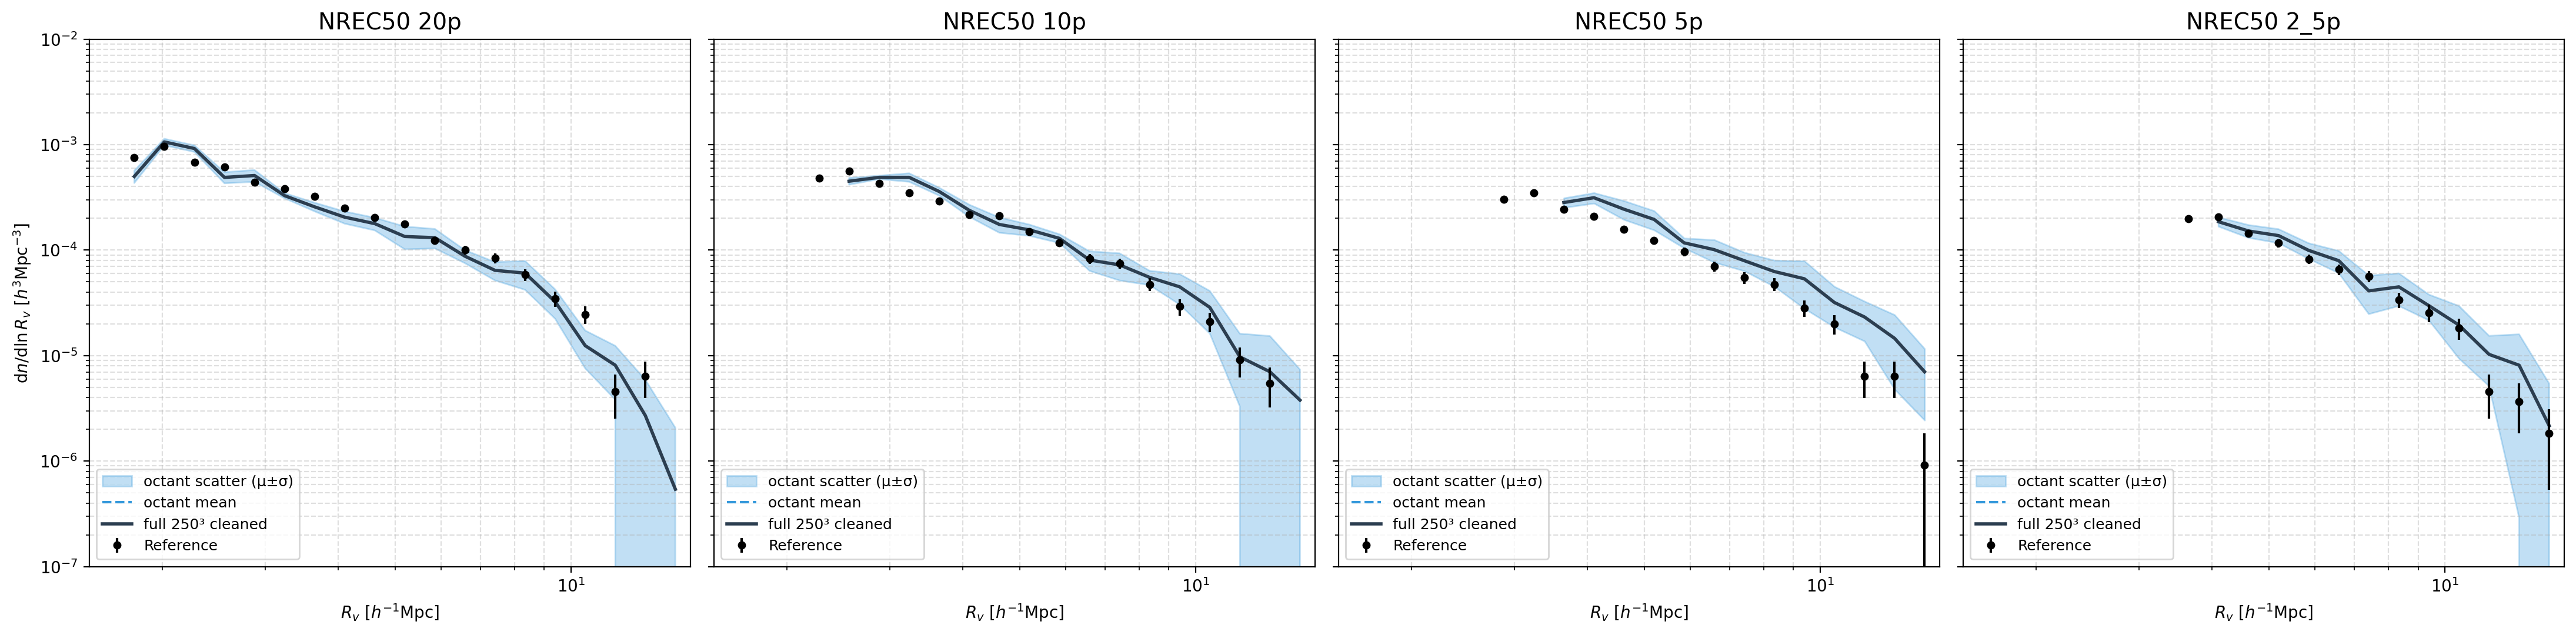
\includegraphics[width=0.90\textwidth]{variance_octants}
    \caption{
    Empirical intra-realisation variance estimated by dividing the simulation box into eight octants and recomputing the VSF in each subvolume. The scatter between octants is modest for the dense samples but grows significantly for the sparse ones, especially near the peak of the VSF. This demonstrates that finite-volume fluctuations contribute non-negligibly to the uncertainty budget, even before considering independent realisations.
    }
    \label{fig:variance_octants_results}
\end{figure}

\begin{figure}[H]
    \centering
    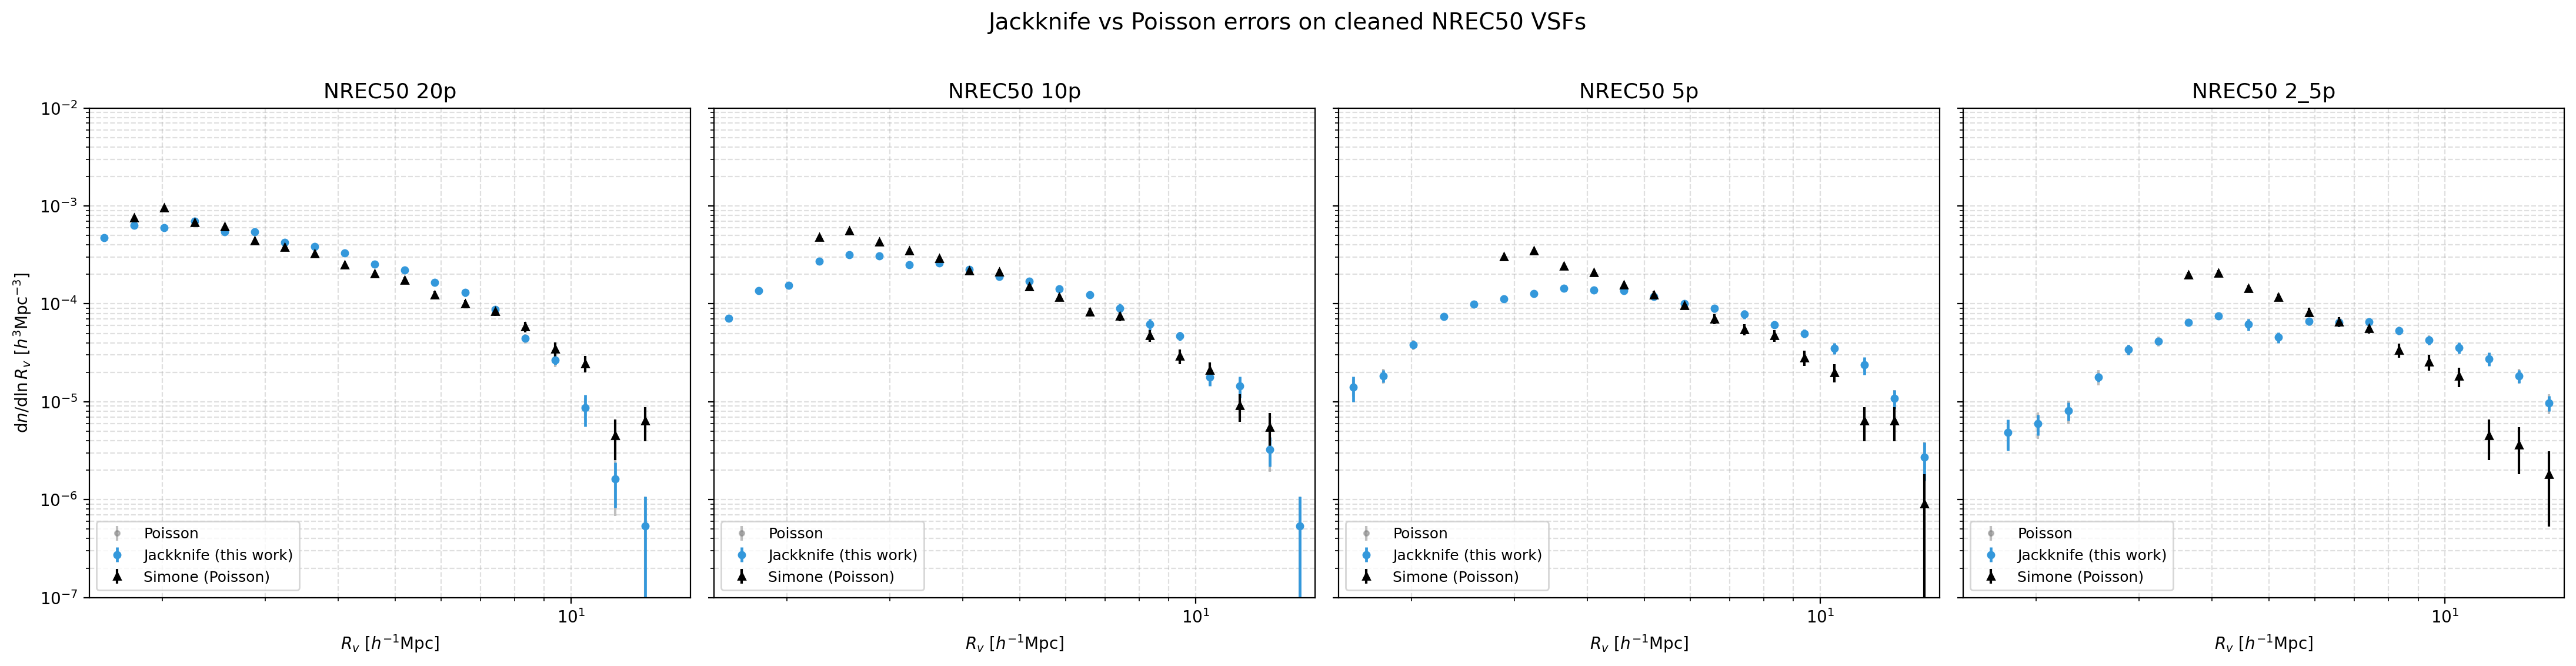
\includegraphics[width=0.88\textwidth]{jackknife_vs_poisson}
    \caption{
    Comparison between empirical resampling errors and analytic Poisson uncertainties for the VSF. Poisson errors correctly capture the counting-noise floor but underestimate the total uncertainty in the bins most affected by cleaning correlations and finite-volume fluctuations. The difference is largest in the sparse catalogues, where the small number of resolved voids and the steep cleaning-induced selection both amplify the non-Poisson component.
    }
    \label{fig:jackknife_poisson_results}
\end{figure}

These figures show that Poisson errors should be interpreted as lower limits, not as complete uncertainty estimates. In the dense catalogues they remain a reasonable first approximation, but in the 5\% and 2.5\% samples the additional variance from finite volume and cleaning correlations is visibly non-negligible. This result directly feeds into the cosmological analysis: if the likelihood overweights the small-radius bins using diagonal Poisson errors alone, the MCMC will react to realisation-specific features as though they were precise cosmological information.

\subsection{Tracer-Density Stability and the Limits of Universality}

A broader scientific question behind the validation exercise is whether the VSF can be treated as approximately universal across tracer densities once cleaning is applied. Figure~\ref{fig:universality_results} addresses this directly for the BitVF catalogues.

\begin{figure}[H]
    \centering
    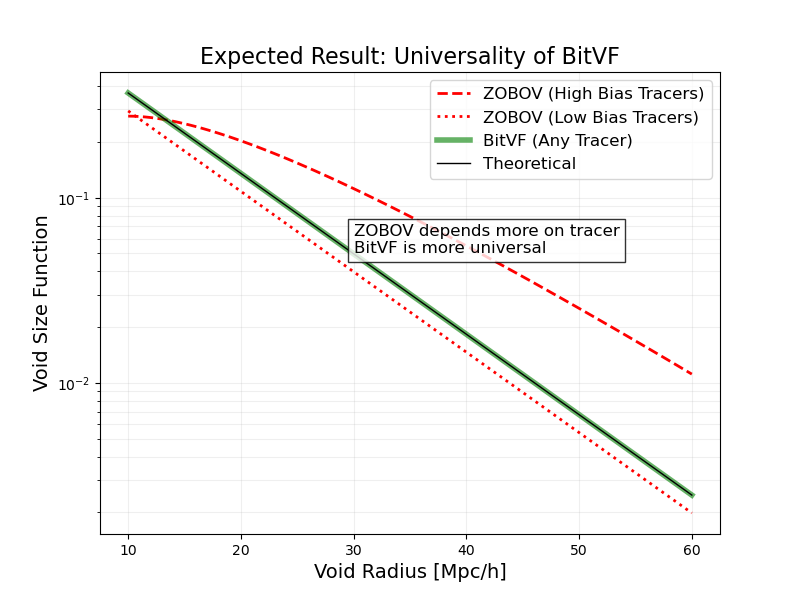
\includegraphics[width=0.90\textwidth]{universatility_bvf}
    \caption{
    Test of approximate universality of the BitVF Void Size Function across tracer densities. The curves do not collapse onto a single universal form: the peak location, low-radius suppression, and overall slope evolve systematically with the sampling fraction. The result confirms that cleaning alone does not erase the imprint of tracer sparsity, although the dynamical BitVF construction keeps the variation controlled enough for meaningful cross-subsample comparison.
    }
    \label{fig:universality_results}
\end{figure}

The curves do not become density-independent after cleaning. Instead, they retain a controlled but unmistakable dependence on tracer sampling, with the characteristic scale moving to larger radii as the catalogues become sparser. This is not surprising given the MPS floor, but it is a useful caution against over-interpreting universality claims. A cleaned VSF is more physically interpretable than a raw watershed output, yet it still remembers how the tracer field sampled the underlying matter distribution.

Taken together, the Phase 1 results support four concrete statements:
\begin{enumerate}
    \item the production cleaning pipeline is consistent with the reference implementation at high tracer density;
    \item the sparse-catalogue mismatch cannot be repaired by further post-processing and is best explained by single-realisation variance relative to an ensemble reference;
    \item Poisson errors underestimate the true uncertainty where cleaning and finite-volume effects are important; and
    \item dynamical and geometric void definitions are physically distinguishable even after common cleaning choices are imposed.
\end{enumerate}

\section{Phase 2: Pre-MCMC Validation of the Vdn Forward Model}
\label{sec:pre_mcmc_results}

\subsection{Theory Versus Data at the Fiducial Cosmology}

Before sampling any cosmological parameters, the Vdn model was evaluated at the true Aletheia cosmology, $\Omega_m = 0.315$ and $\sigma_8 = 0.811$, with the canonical shell-crossing threshold $\delta_v=-2.71$. The result is shown in Figure~\ref{fig:vdn_vs_data_results}.

\begin{figure}[H]
    \centering
    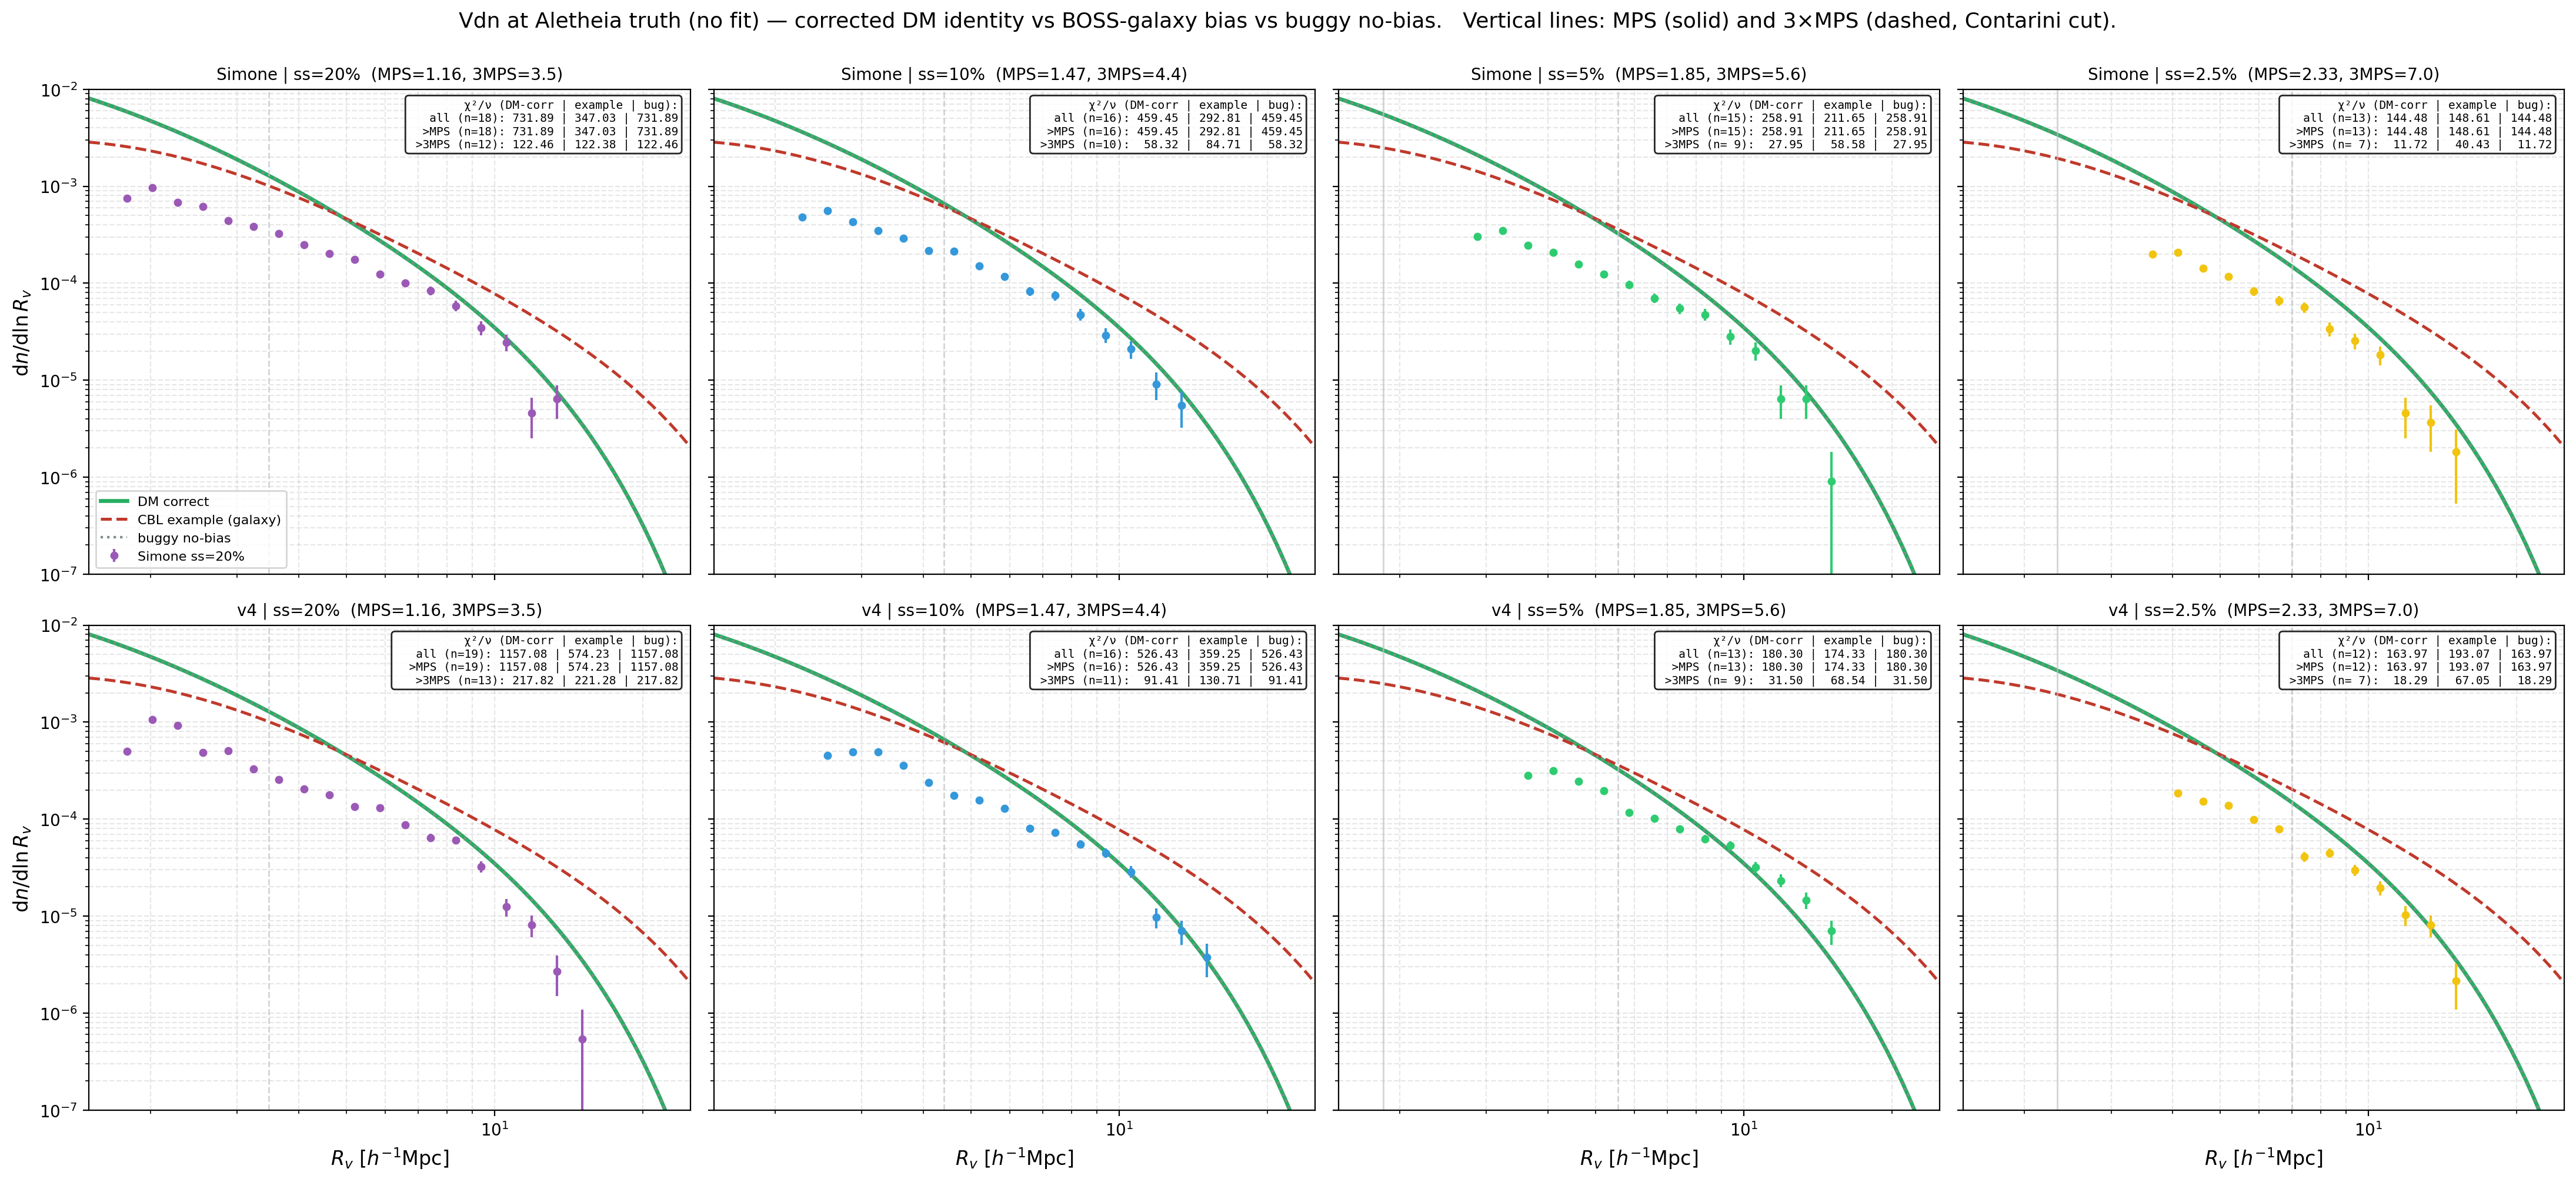
\includegraphics[width=0.92\textwidth]{vsf_theory_vs_data}
    \caption{
    Vdn prediction at the true Aletheia cosmology compared with the empirical VSF data vector. The model reproduces the broad decline at intermediate and large radii, but it fails to match the small-radius regime and does not reproduce the observed peak structure created by the cleaned catalogue. This figure is the central pre-MCMC sanity check: the forward model is not calibrated to the data even before parameter inference begins.
    }
    \label{fig:vdn_vs_data_results}
\end{figure}

This figure is the central calibration result of the thesis. The Vdn curve is not grossly wrong everywhere: at intermediate and large radii it captures the expected downward trend and therefore contains real physical information. However, it systematically misses the detailed shape of the empirical VSF, especially in the small-radius regime where the data exhibit a pronounced peak and curvature that the smooth excursion-set prediction cannot reproduce. The problem is therefore not numerical failure. The problem is that the idealised objects counted by the theory are not yet the same objects as those returned by the cleaned catalogue.

This is exactly the issue highlighted in the presentation feedback. A pipeline can be computationally correct and still be insufficient for cosmological inference if the data vector entering the likelihood has not been calibrated against the forward model at the known cosmology. Figure~\ref{fig:vdn_vs_data_results} shows that such a calibration step is necessary here.

\subsection{Residual Structure of the Model Mismatch}

The misfit becomes clearer when plotted as residuals, as in Figure~\ref{fig:vdn_residuals_results}.

\begin{figure}[H]
    \centering
    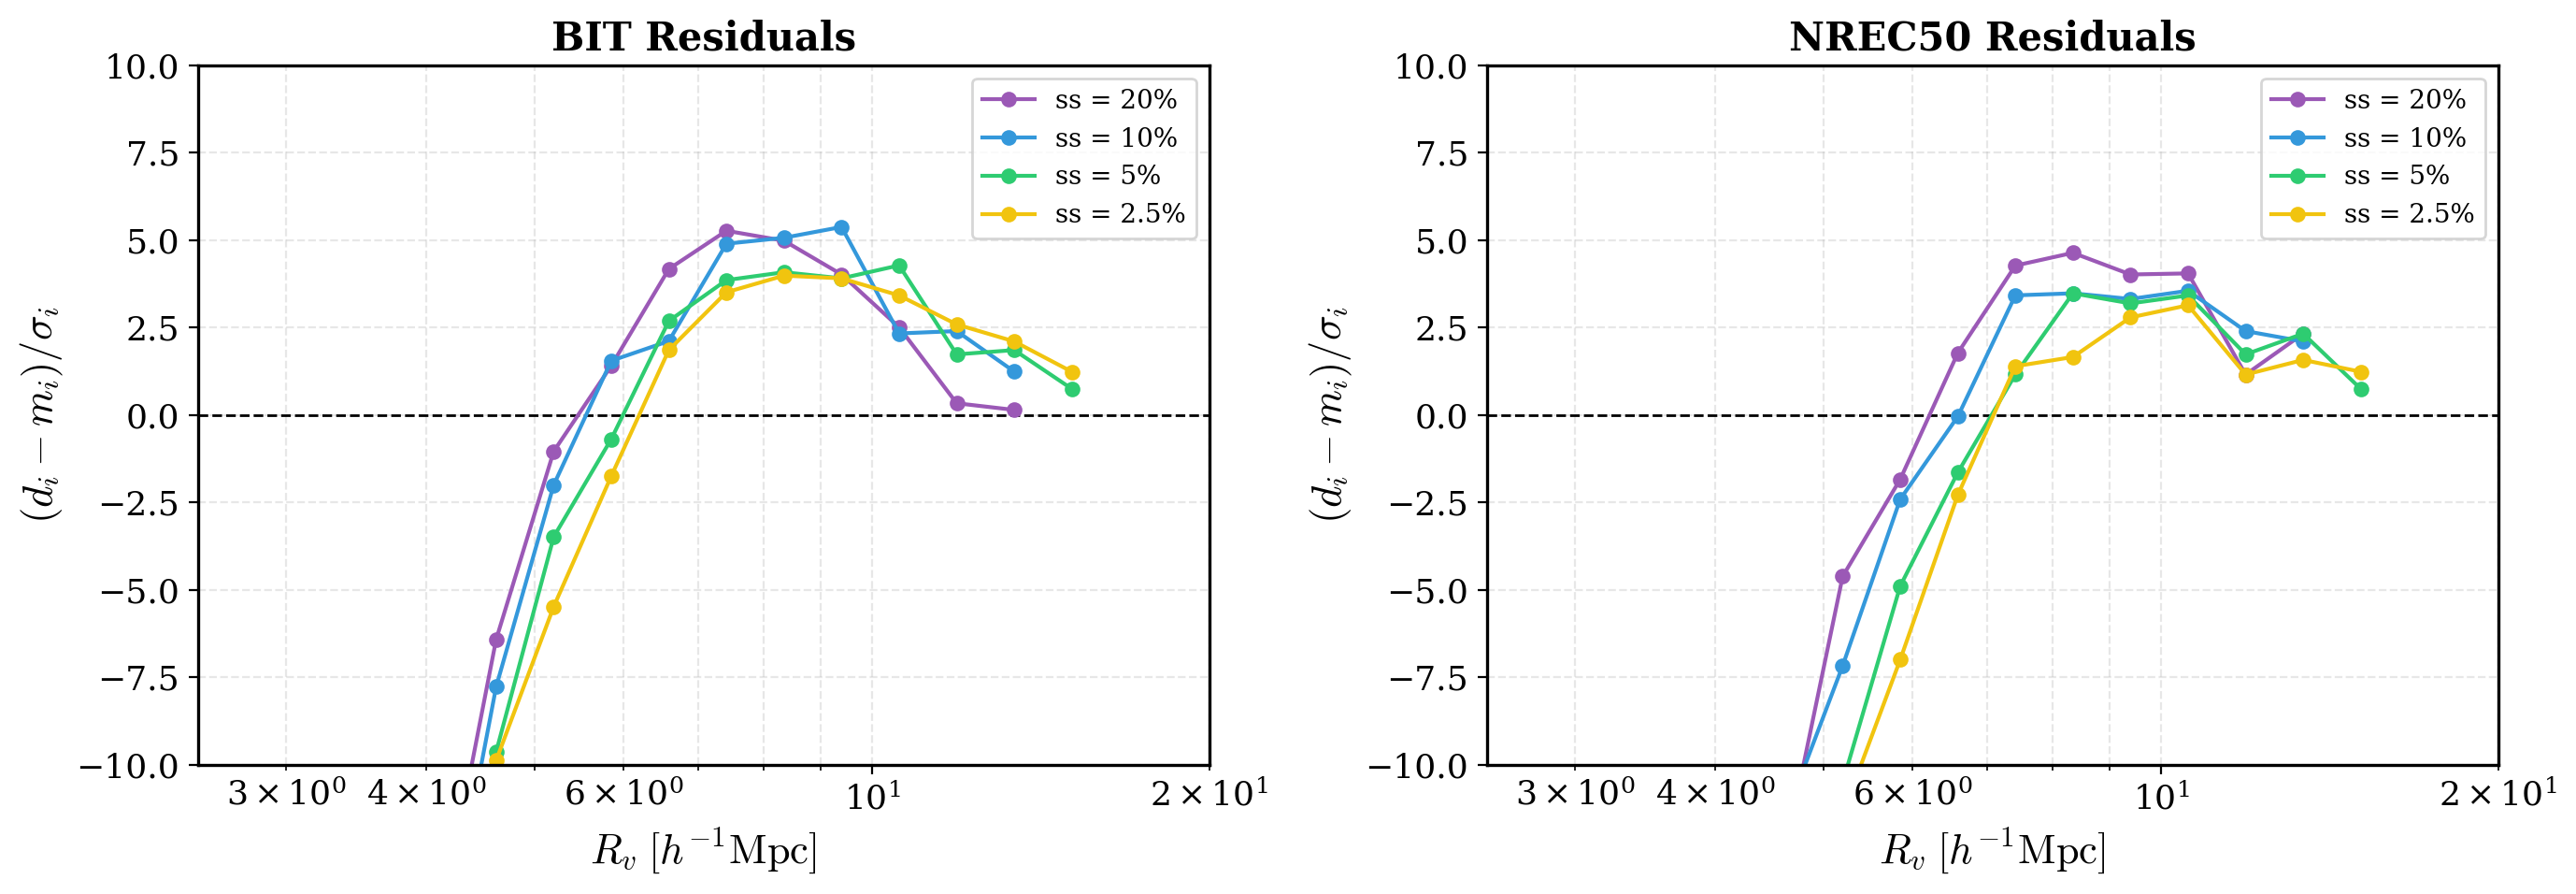
\includegraphics[width=0.88\textwidth]{vsf_residuals}
    \caption{
    Residuals between the fiducial-cosmology Vdn prediction and the empirical VSF. The residual pattern is highly structured rather than noise-like: the model overpredicts the smallest radii, underpredicts the intermediate-radius peak, and only approaches consistency at the largest radii. Such a coherent pattern indicates a shape mismatch between theory and cleaned data, not a fluctuation that can be absorbed by parameter shifts alone.
    }
    \label{fig:vdn_residuals_results}
\end{figure}

The residuals are strongly non-random. Small voids are overpredicted, intermediate radii are underpredicted, and only the largest voids show approximate agreement. This sign-changing structure is exactly what one expects from a model that lacks an explicit treatment of exclusion, finite tracer resolution, and cleaning-induced reshaping of the catalogue. A simple shift in $\Omega_m$ or $\sigma_8$ can move the curve up or down and slightly alter its slope, but it cannot create the missing peak structure.

\subsection{Changing the Nonlinear Threshold Shifts the Curve but Does Not Fix the Shape}

One possible explanation for the mismatch would be that the nonlinear density threshold used in the Lagrangian-to-Eulerian mapping is simply mis-specified. Figure~\ref{fig:delta_nl_scan_results} tests this possibility by varying $\delta_\mathrm{NL}$.

\begin{figure}[H]
    \centering
    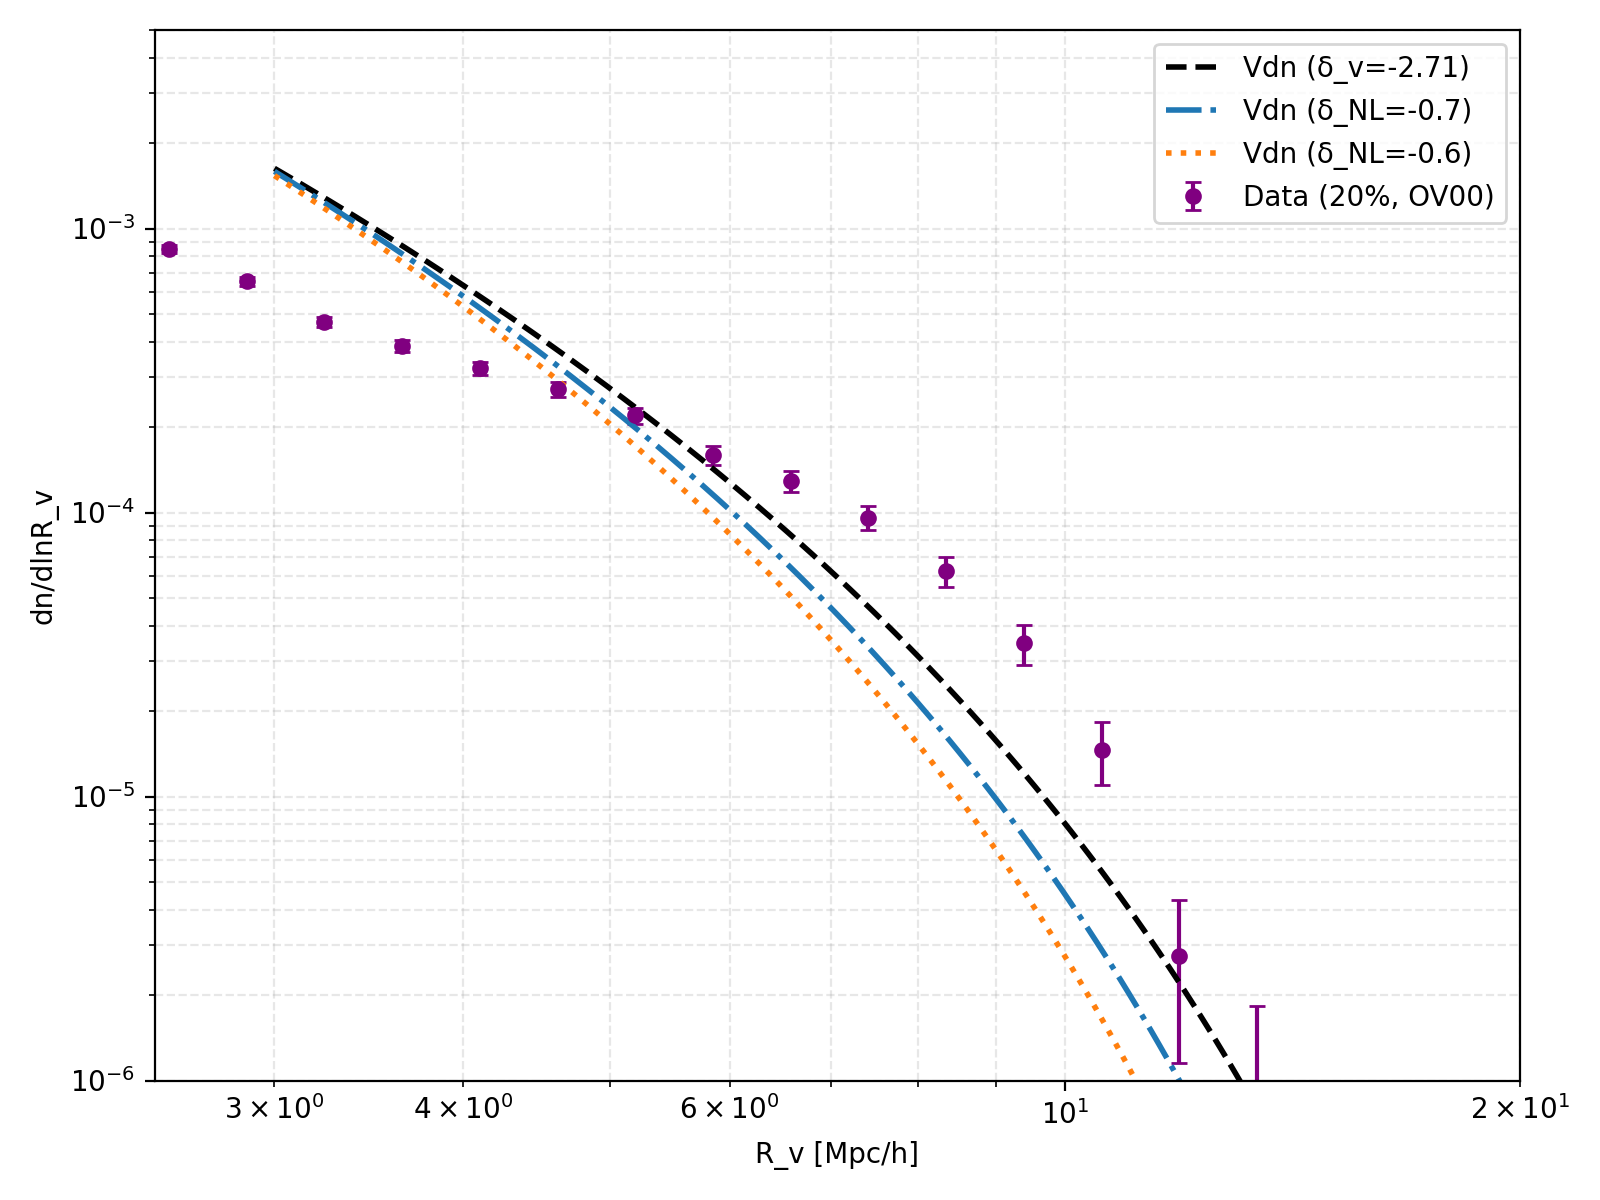
\includegraphics[width=0.88\textwidth]{vsf_delta_nl_scan}
    \caption{
    Scan of the nonlinear density threshold used in the Lagrangian-to-Eulerian mapping of the Vdn model. Changing $\delta_\mathrm{NL}$ primarily shifts the theoretical curve horizontally by altering the expansion factor between $R_L$ and $R_E$. It does not reproduce the observed bump and therefore cannot, by itself, calibrate the model to the cleaned data vector.
    }
    \label{fig:delta_nl_scan_results}
\end{figure}

The result is unambiguous: adjusting $\delta_\mathrm{NL}$ shifts the prediction in radius but leaves the basic shape essentially intact. This confirms that the main problem is not a single wrong threshold value. The mismatch instead resides in the mapping between idealised theoretical voids and the actual catalogue produced by the finite-resolution, overlap-pruned pipeline.

\section{Phase 2: Behaviour of the MCMC Fits}
\label{sec:results_mcmc}

\subsection{Pilot Fits and the Need for a Nuisance Parameter}

The progressive local tests performed before the cluster runs already showed that a naive two-parameter fit is inadequate. When only $\Omega_m$ and $\sigma_8$ are allowed to vary and all bins are included, the chains run to the prior boundaries because the model attempts to compensate for its shape mismatch by pushing the cosmological parameters to extreme values. Restricting the fit to $R>6\,h^{-1}\mathrm{Mpc}$ improves convergence but does not remove the bias. This motivated the adoption of a three-parameter production model in which $\delta_v$ is allowed to float as a nuisance parameter.

The best-fit logic behind this choice is illustrated in Figure~\ref{fig:bestfit_compare_results}, which compares the fiducial and fitted curves for representative runs.

\begin{figure}[H]
    \centering
    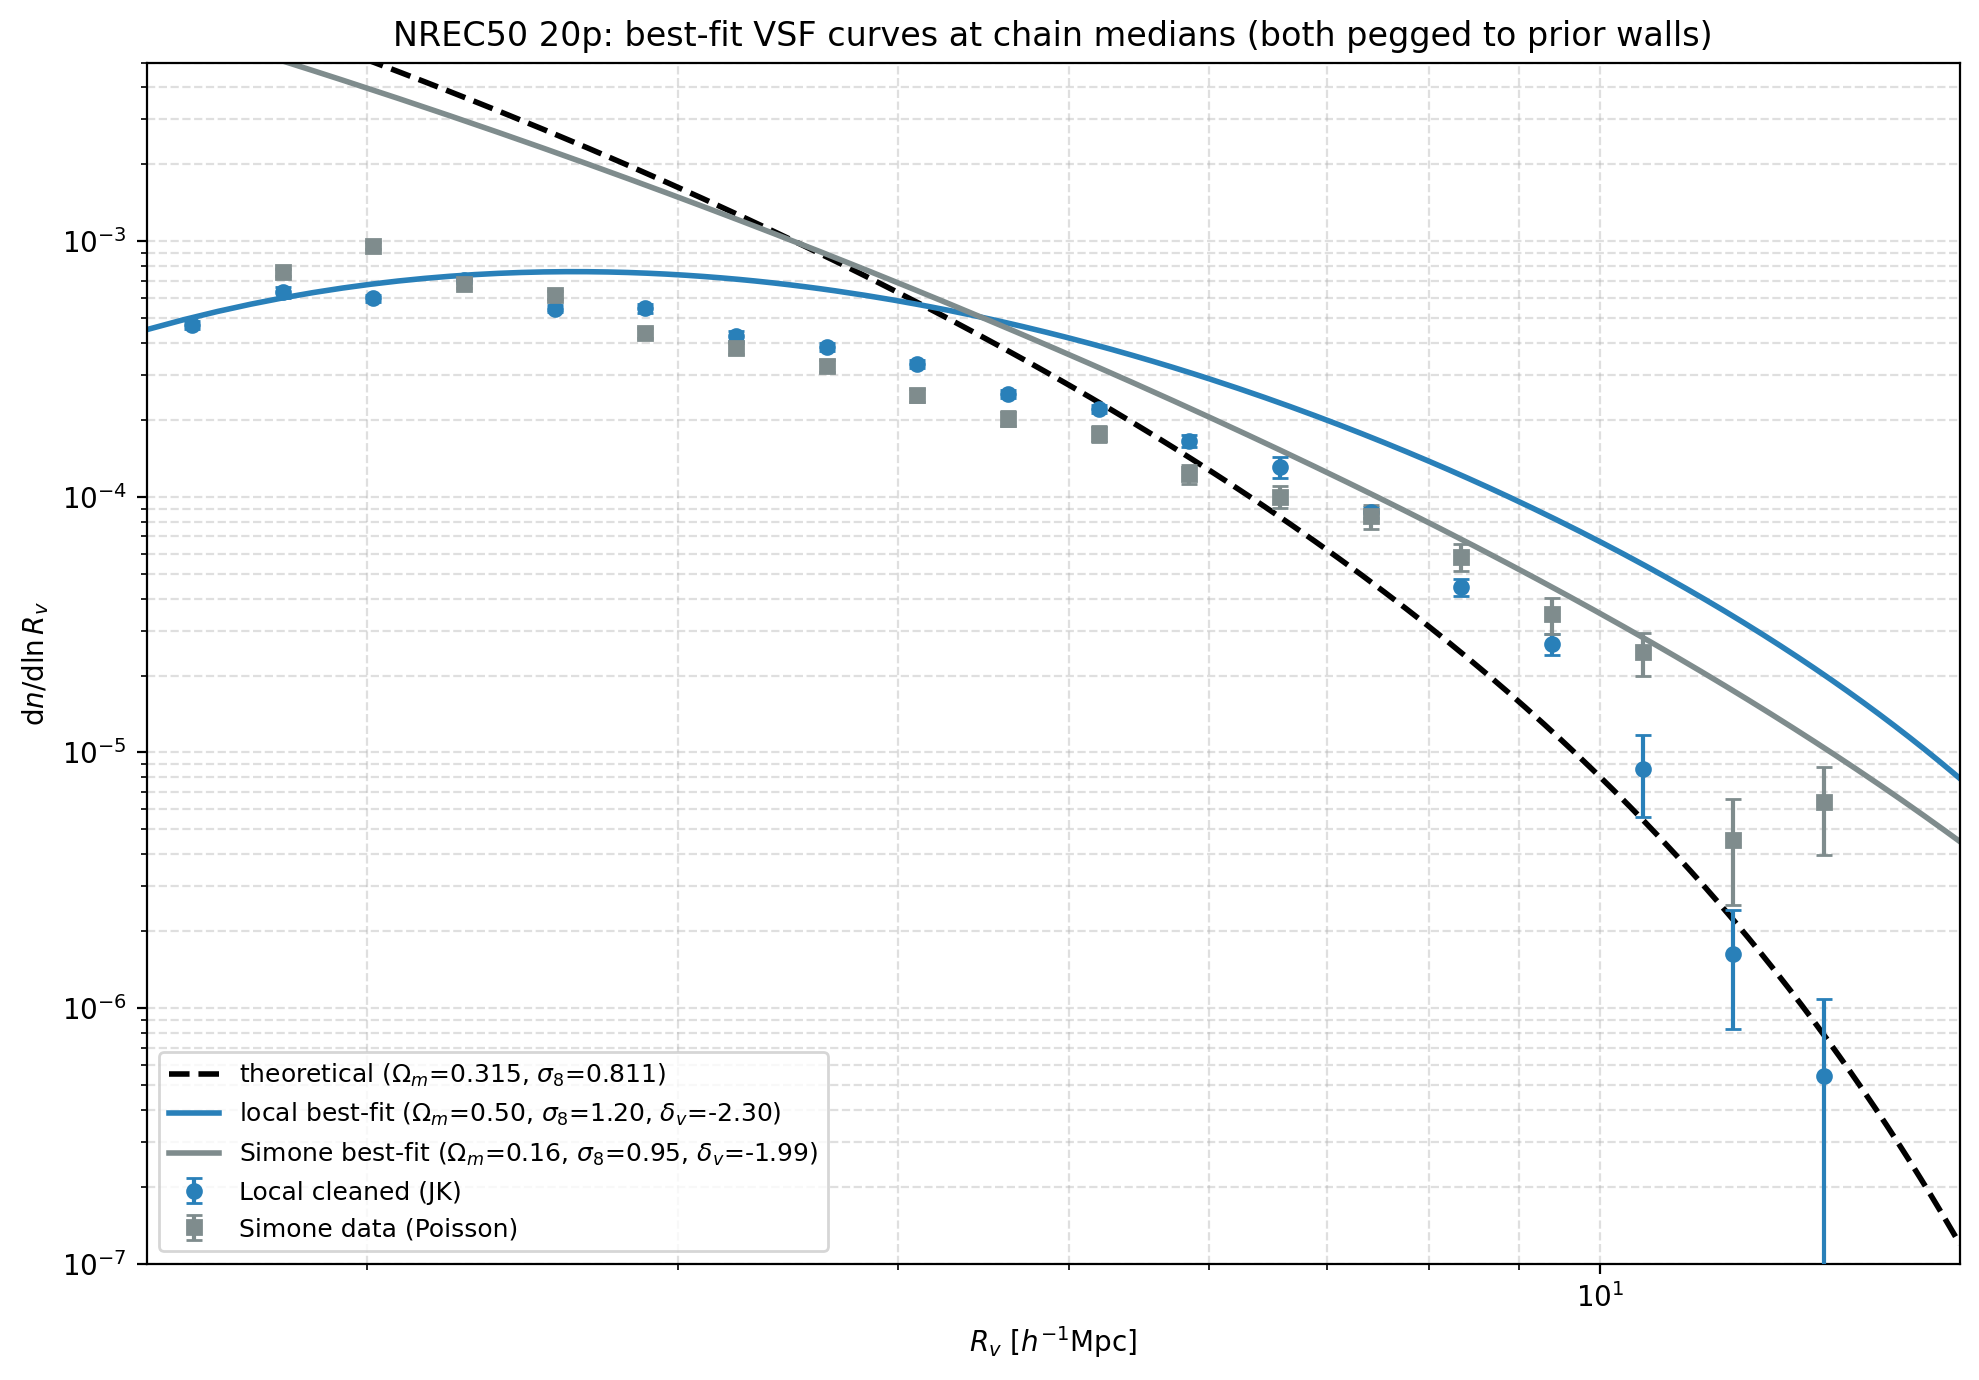
\includegraphics[width=0.92\textwidth]{bestfit_compare}
    \caption{
    Representative comparison between the empirical data vector, the fiducial-cosmology Vdn prediction, and the MCMC best-fit curve. Allowing the sampler to vary the parameters improves the match in the intermediate-radius regime, but no fit removes the basic structural discrepancy visible at small radii. The best fit therefore reflects compensation for model error rather than a faithful recovery of the true cosmology.
    }
    \label{fig:bestfit_compare_results}
\end{figure}

\subsection{Production-Run Summary}

The eight production runs sample all combinations of two reconstruction fields (BIT and NREC50) and four tracer subsamples (20\%, 10\%, 5\%, 2.5\%). Their marginal constraints are summarised in Table~\ref{tab:production_results}. The full chain-level diagnostics will be documented in Appendix~\ref{app:mcmc_summary} in the final version of the thesis.

\begin{table}[H]
    \centering
    \caption{Summary of the eight production 3D MCMC runs. Quoted intervals are the approximate marginalized constraints extracted from the cluster analysis. The true Aletheia values are $\Omega_m=0.315$, $\sigma_8=0.811$, and $\delta_v=-2.71$.}
    \label{tab:production_results}
    \begin{tabular}{lccc}
        \toprule
        \textbf{Run} & \textbf{$\Omega_m$} & \textbf{$\sigma_8$} & \textbf{$\delta_v$} \\
        \midrule
        BIT 20\%   & $0.10^{+0.07}_{-0.00}$ & $0.75^{+0.45}_{-0.11}$ & $-2.60^{+1.10}_{-0.78}$ \\
        BIT 10\%   & $0.12^{+0.09}_{-0.02}$ & $0.87^{+0.33}_{-0.15}$ & $-2.67^{+1.17}_{-0.76}$ \\
        BIT 5\%    & $0.10^{+0.00}_{-0.00}$ & $0.97^{+0.03}_{-0.08}$ & $-3.39^{+0.28}_{-0.09}$ \\
        BIT 2.5\%  & $0.10^{+0.01}_{-0.00}$ & $1.13^{+0.05}_{-0.09}$ & $-3.40^{+0.22}_{-0.07}$ \\
        NREC50 20\%  & $0.11^{+0.12}_{-0.01}$ & $0.68^{+0.52}_{-0.11}$ & $-2.72^{+1.22}_{-0.61}$ \\
        NREC50 10\%  & $0.10^{+0.02}_{-0.00}$ & $0.68^{+0.10}_{-0.13}$ & $-2.85^{+0.56}_{-0.50}$ \\
        NREC50 5\%   & $0.10^{+0.00}_{-0.00}$ & $0.74^{+0.12}_{-0.16}$ & $-2.96^{+0.59}_{-0.40}$ \\
        NREC50 2.5\% & $0.10^{+0.00}_{-0.00}$ & $0.84^{+0.13}_{-0.20}$ & $-2.89^{+0.70}_{-0.47}$ \\
        \bottomrule
    \end{tabular}
\end{table}

The dominant pattern in Table~\ref{tab:production_results} is immediate: $\Omega_m$ is driven to the lower prior boundary in every run. This is the clearest signal that the sampler is compensating for structural model mismatch rather than recovering the true cosmology. By contrast, $\sigma_8$ performs substantially better, especially for the NREC50 catalogues, where several runs recover the true value within approximately one standard deviation. The nuisance parameter $\delta_v$ remains near the physically expected excursion-set range, indicating that the 3D parameterisation is sensible even though the cosmological recovery is biased.

\subsection{Representative Posterior Diagnostics}

To illustrate the chain behaviour, Figures~\ref{fig:trace_example_results} and~\ref{fig:corner_example_results} show representative diagnostics from the NREC50 2.5\% and NREC50 20\% runs, respectively.

\begin{figure}[H]
    \centering
    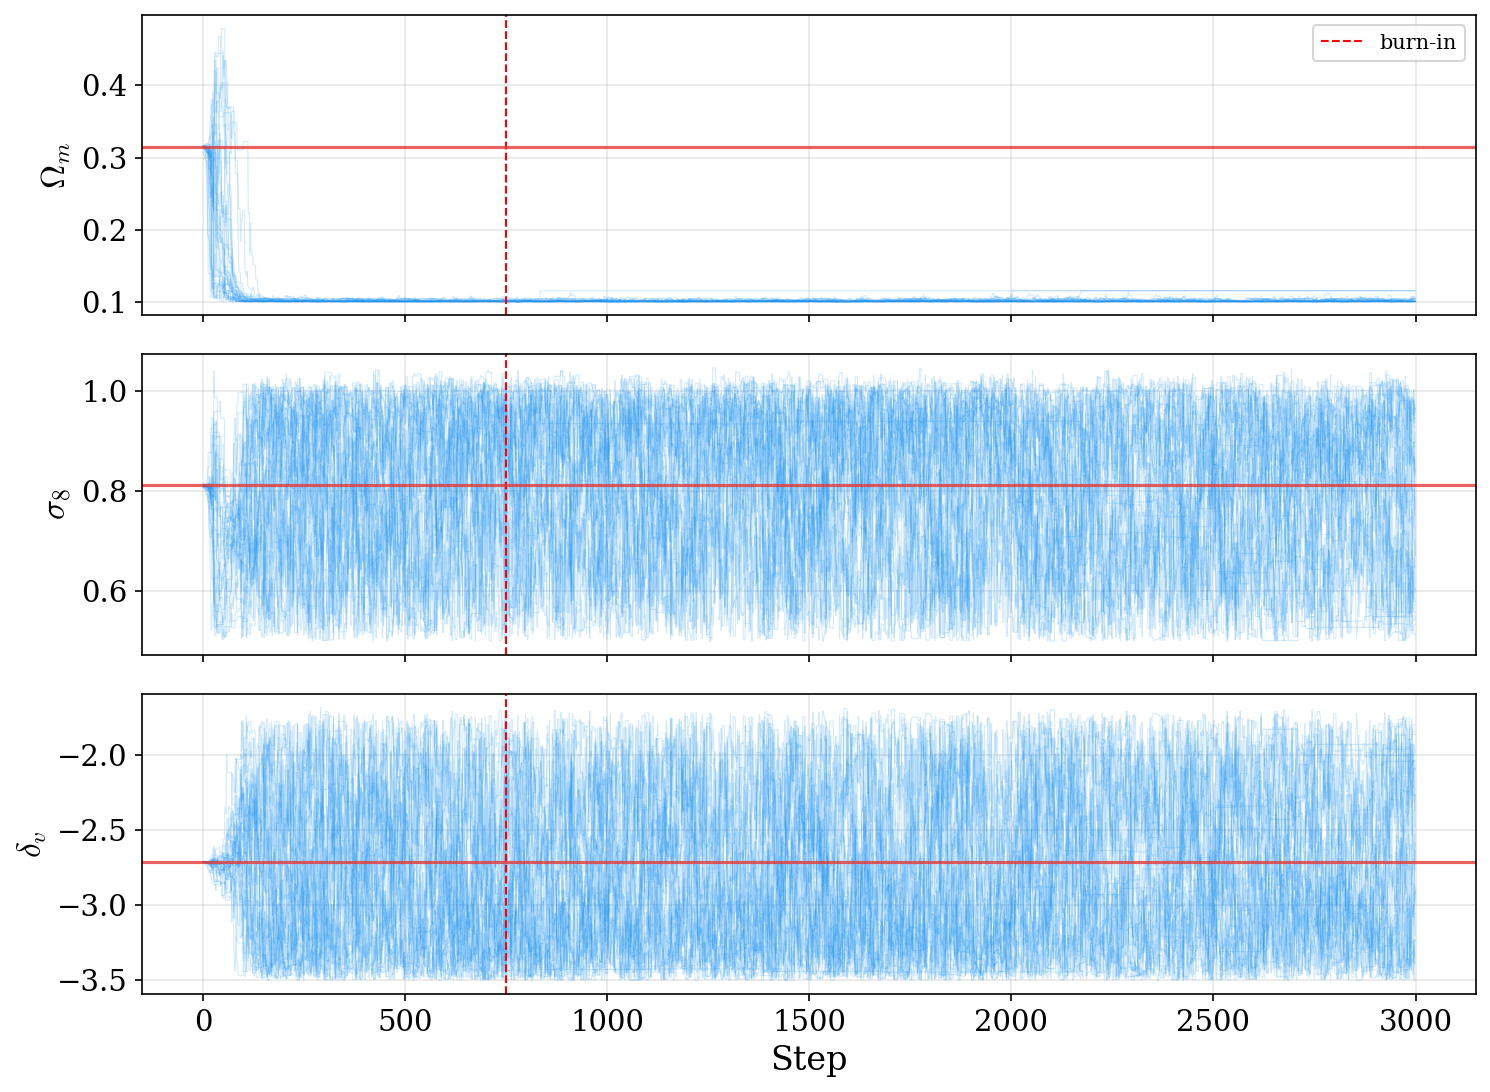
\includegraphics[width=0.88\textwidth]{traces_NREC50_2_5p_3D}
    \caption{
    Representative trace plot for the NREC50 2.5\% production run. The chains for $\sigma_8$ and $\delta_v$ mix reasonably well, while $\Omega_m$ rapidly collapses to the lower prior boundary and remains there. This is a diagnostic of model preference, not of numerical non-convergence.
    }
    \label{fig:trace_example_results}
\end{figure}

\begin{figure}[H]
    \centering
    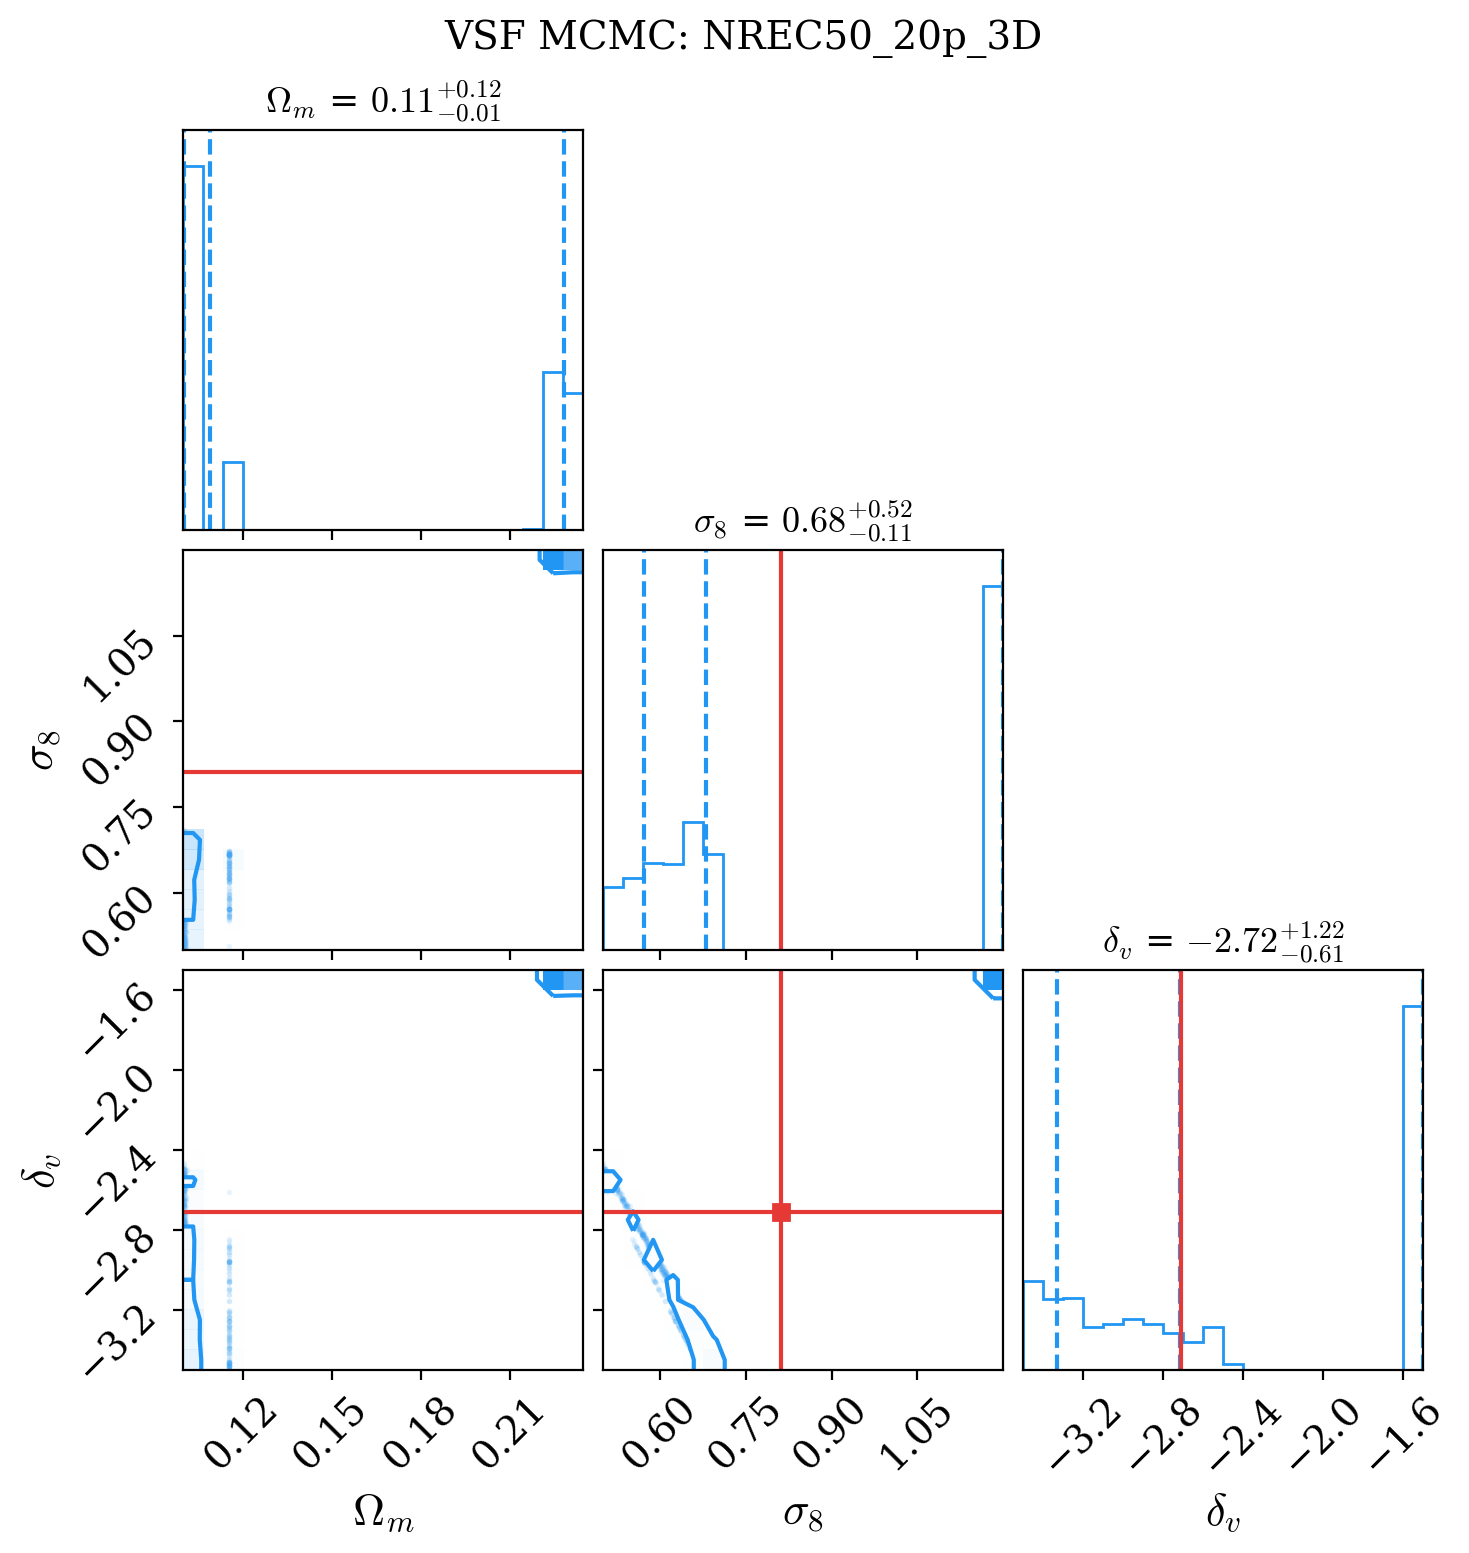
\includegraphics[width=0.82\textwidth]{corner_NREC50_20p_3D}
    \caption{
    Representative corner plot for a production 3D fit. The posterior shows an extended degeneracy between $\Omega_m$, $\sigma_8$, and $\delta_v$, with the marginalized probability concentrated against the $\Omega_m$ prior floor. The true cosmology is not recovered despite acceptable-looking sampler behaviour, demonstrating that convergence diagnostics alone are insufficient when the forward model is uncalibrated.
    }
    \label{fig:corner_example_results}
\end{figure}

These diagnostics are useful because they separate numerical behaviour from scientific validity. The chains mix well enough to show that the sampler is working as intended, but the posterior still concentrates in the wrong place. In this project, the issue is therefore not a broken MCMC implementation. The issue is that the Vdn model cannot reproduce the measured VSF shape without pushing part of the parameter space to an unphysical edge.

\subsection{Results-Level Interpretation}

The production MCMC outputs support a simple conclusion. The inference machinery runs, but the answer it gives should not be interpreted as a cosmological measurement. The Vdn implementation evaluates correctly, the likelihood is well-defined, and the \texttt{emcee} chains settle into stable posterior structure. Even so, the underlying model is not calibrated to the measured VSF. The catalogue entering the fit carries the imprint of finite tracer resolution, overlap pruning, and single-realisation variance, and the basic Vdn model does not absorb those effects.

This is why the pre-MCMC sanity check matters so much in this thesis. Without it, the posterior might have been misread as evidence for a low $\Omega_m$ cosmology. After the sanity check, that interpretation is no longer defensible. What the fit is really showing is the cost of using an uncalibrated forward model.

\section{Summary of Results}

The results of this stage of the thesis can be summarised as follows:
\begin{enumerate}
    \item The production BitVF cleaning and VSF pipeline is validated against the reference implementation of \citet{Sartori2025}, especially for the denser 20\% and 10\% tracer catalogues.
    \item The residual low-density mismatch with the Simone\_data reference is already present in the raw catalogues and is best interpreted as a single-realisation versus ensemble-average effect, not as a cleaning bug.
    \item Empirical variance estimates show that Poisson uncertainties underestimate the full error budget in the sparse and aggressively cleaned regimes.
    \item The fiducial Vdn model does not match the empirical VSF at the true Aletheia cosmology; the mismatch is structured and persists under threshold scans.
    \item The MCMC framework converges technically, but the posteriors are biased because the uncalibrated forward model compensates for shape mismatch by driving $\Omega_m$ to the prior floor.
\end{enumerate}

These findings set up the next stage of the thesis naturally. The central task is no longer to debug the pipeline, but to interpret what these validated-yet-biased results imply for cosmological inference, model calibration, and future dynamical void analyses.

\chapter{Discussion}
\label{chap:discussion}

\section{What Was Established by This Work}

The first main outcome of this thesis is methodological. I built the BitVF-based analysis chain, tested it against the available reference products, and pushed it far enough to see where it holds and where it stops being trustworthy. That chain includes cleaning, overlap removal, border handling, VSF computation, comparison to Simone\_data, pre-MCMC model checks, and full production inference runs. This matters because the VSF is not a raw observable; it depends strongly on how the final void catalogue is operationally defined.

The second main outcome is that a validated measurement chain is still not enough for cosmological inference. The cleaned VSF is reproducible as a data product, but that does not mean the chosen forward model is already calibrated to it. In this thesis, two conditions need to be separated:
\begin{enumerate}
    \item the catalogue and statistic must be internally consistent and reproducible; and
    \item the theoretical model must match that statistic at the known fiducial cosmology before cosmological parameters are floated.
\end{enumerate}
This thesis satisfies the first condition and fails the second. That failure is still useful, because it identifies the remaining bottleneck clearly instead of hiding it behind a clean-looking posterior.

\section{Interpretation of the Phase 1 Validation Results}

The Phase 1 results show that the production cleaning prescription is basically sound. In the 20\% and 10\% NREC50 samples, the locally measured VSF follows the Simone\_data reference closely enough in both peak location and overall shape for the implementation to be considered validated. The sparse-sample mismatch is more informative than the good agreement, because it survives every reasonable downstream change to the cleaning setup.

That matters for two reasons. First, it shows that the 5\% and 2.5\% catalogues are already in a high-variance regime before the final cleaning choices are applied. Second, it suggests that the reference product contains information about generation protocol, not only cleaning convention. The raw local catalogue is already low near the peak, so the discrepancy cannot be created later by overlap removal or border cuts. The simplest interpretation is that a single local realization is being compared against an ensemble-level reference.

The octant and jackknife checks are important here because they support that reading quantitatively. In the sparse regime, Poisson bars are too optimistic. The problem is not only low counts. The bins are also shaped by overlap pruning and finite-volume fluctuations, so treating them as independent Poisson measurements overstates the precision of the data vector.

\section{Interpretation of the Vdn Mismatch}

The pre-MCMC comparison between the empirical VSF and the Vdn prediction at the Aletheia cosmology is the central interpretive result of the thesis. The mismatch is not a small local defect. It has structure: too many small voids in the model, a missed feature around the measured peak, and better agreement only toward the large-radius tail.

That pattern is physically plausible once one remembers what is being compared. The Vdn curve describes an idealized abundance of shell-crossed, non-overlapping voids in a smoothed field. The measured catalogue is the result of reconstruction, thresholding, radius definition, overlap pruning, and finite sampling. Those are not minor implementation details; they define the actual objects being counted. The later MCMC bias is already encoded in this mismatch.

The $\delta_\mathrm{NL}$ scans make the point sharper. If the problem were only the nonlinear density threshold, changing that threshold would have repaired the fit. Instead, the curve mainly shifts in radius while the shape problem remains. So the missing ingredient is not a single number. It is a better mapping from the theoretical void population to the pipeline-defined one.

\section{Why Matter Density Fails While Fluctuation Amplitude Often Survives}

One of the clearest patterns in the production runs is the difference between $\Omega_m$ and $\sigma_8$. The $\Omega_m$ posterior repeatedly piles up at the lower prior edge, whereas $\sigma_8$ remains much more reasonable, especially for NREC50. That asymmetry is more informative than any single central value.

My reading is that $\Omega_m$ is acting as the parameter the sampler can use to reshape the theoretical curve most aggressively. Since the model cannot reproduce the observed peak directly, the posterior uses $\Omega_m$ to flatten or reweight the prediction in the least bad direction. In that sense, $\Omega_m$ is not being measured cleanly; it is absorbing model error. The behaviour of $\sigma_8$ is different because the VSF still retains a more direct sensitivity to overall fluctuation amplitude even when the detailed shape is wrong.

The nuisance parameter $\delta_v$ also helps interpret the fit. It does move, but usually within a range that still makes physical sense for an excursion-set barrier. So the three-parameter model is not completely unconstrained. The problem is narrower: one parameter combination is being used to compensate for structural mismatch that the model itself should have handled.

\section{Dynamical Versus Geometric Void Definitions}

An important theme running through the thesis is the difference between geometric and dynamical void definitions. In my results, BitVF is not just another code that makes similar curves. It produces a genuinely different route to the VSF because it starts from reconstructed mass flow instead of tracer-space density basins.

That difference helps, but it does not solve everything. A dynamical definition can reduce some of the obvious tracer-space artefacts, yet the final cosmological statistic still depends on reconstruction quality, cleaning, and the way the catalogue is matched to theory. In other words, switching from REVOLVER-like geometry to BitVF dynamics improves the measurement side, but it does not automatically fix the theory side.

This is the point at which the current thesis stops and the next stage begins. The pipeline is far enough along to justify a more accurate modelling step, not just more implementation debugging.

\section{Relation to the Presentation Feedback}

The presentation feedback was that the pipeline itself looked solid, but the data should have been calibrated because the pre-MCMC plots already disagreed with Vdn. After completing the later chapters, I agree with that assessment. The disagreement is not a side remark. It is the main reason the posterior cannot be interpreted literally.

At the same time, the MCMC stage was still worth doing. It shows what happens when this calibration step is skipped. The chains do not crash. The sampler does not look obviously broken. Instead, the posterior quietly develops a pathological preference for the edge of prior space. That is a much more useful lesson than a simple statement that the theory curve is imperfect.

\section{Limitations of the Present Study}

Several limitations should be kept explicit.

\begin{enumerate}
    \item The analysis is based on a single $250\,h^{-1}\mathrm{Mpc}$ simulation box, so inter-realisation covariance is not directly measured.
    \item The sparse-subsample comparison depends on local single-realisation catalogues versus a likely ensemble-averaged Simone\_data reference, which limits strict one-to-one reproducibility.
    \item The likelihood uses diagonal Poisson uncertainties rather than a full covariance matrix, which overweights bins affected by cleaning correlations and finite-volume effects.
    \item The Vdn model is an intentionally simple analytical forward model. It is valuable as a diagnostic baseline, but it does not represent the current state of the art for precision void abundance modelling.
    \item The full pipeline-to-theory calibration step, as implemented in observational analyses such as \citet{Contarini2023}, was not completed here.
\end{enumerate}

These limitations do not invalidate the work. They define the boundary conditions under which its conclusions should be read: the thesis is a rigorous validation-and-diagnosis study that prepares the ground for a calibrated cosmological analysis, rather than a final precision-constraint paper.

\chapter{Conclusion}
\label{chap:conclusion}

This thesis used the Aletheia simulation to test a concrete void-analysis workflow rather than to present a final cosmological measurement. The two main goals were to validate the BitVF-based cleaning and VSF pipeline, and to check whether an analytical Vdn model was already adequate for inference on that measured statistic.

The first goal was largely achieved. The final cleaning prescription reproduces the Simone\_data reference well in the denser subsamples, and the later diagnostics show that the remaining sparse mismatch originates before the final cleaning stage. That makes the Phase 1 pipeline defensible as a measurement workflow.

The second goal produced a negative but useful result. The pre-MCMC sanity check shows that the Vdn prediction does not match the measured VSF at the true Aletheia cosmology. Once that mismatch is carried into the likelihood, the posterior responds by pushing $\Omega_m$ to the lower prior boundary. The MCMC therefore runs correctly, but the cosmological interpretation does not.

The main conclusion is straightforward. In this workflow, calibration is not a refinement to be added later; it is a requirement for interpreting the posterior at all. The thesis is useful because it demonstrates that point with a fully working measurement pipeline and a fully working, but not yet trustworthy, inference stage.

\chapter{Future Work}
\label{chap:future_work}

\section{Immediate Next Steps}

The most immediate next step is to add the missing calibration layer between the cleaned BitVF catalogue and the forward model. In practice, this means working with a matched ensemble of realizations processed through the same cleaning pipeline so that the average offset between theory and measurement can be estimated at a known cosmology.

The next requirement is a proper covariance matrix. Poisson errors were enough to expose the main problem, but they are not enough for a serious final fit. The sparse bins, in particular, need an uncertainty model that includes cleaning correlations and finite-volume scatter instead of only counting noise.

\section{Theory Improvements}

The forward model should also be improved. The most obvious comparison is against the moving-barrier framework of \citet{Verza2024}, because the main failure here is not zero cosmological sensitivity but a shape mismatch that Vdn cannot absorb. A model that captures the measured peak and exclusion effects more faithfully may already change the outcome substantially.

More generally, the mapping between theoretical voids and measured voids should be modeled more explicitly. In this thesis, $\delta_v$ was allowed to float as a nuisance parameter, but that is only a coarse way of absorbing pipeline effects. A calibrated transfer function or radius-dependent correction would be more honest about what the measurement process is doing to the abundance curve.

\section{BitVF-Specific Developments}

On the algorithmic side, BitVF itself offers several opportunities for improvement. The sparse-sample mismatch suggests that the stochastic properties of the Optimal Transport reconstruction should be studied more systematically across random seeds, smoothing choices, and reconstruction settings. A controlled realisation suite would help distinguish tracer-sampling variance from reconstruction variance.

The bias-correction step discussed in Appendix~\ref{app:bias_correction} also deserves fuller exploration. In the present thesis it is treated conceptually, but a future study could test whether an explicit, scale-dependent, or environment-dependent bias correction further stabilises the recovered VSF. If successful, this would strengthen the case that dynamical void definitions can reduce tracer-space systematics in a practically useful way.

\section{Extending the Scope of the Analysis}

Once calibration and covariance are improved, several straightforward extensions become possible.

\begin{enumerate}
    \item Perform the full production inference using multiple cosmological simulations rather than a single fiducial box, allowing actual recovery tests instead of one-cosmology validation.
    \item Extend the parameter space beyond $(\Omega_m,\sigma_8)$ to include combinations such as $S_8$, dark-energy parameters, modified-gravity parameters, or neutrino mass, where voids are expected to be especially informative.
    \item Compare the VSF constraints directly with other void observables such as density profiles, void--galaxy correlations, and lensing signals to test multi-probe consistency.
    \item Apply the validated pipeline to survey-like mock catalogues with realistic masks, selection functions, and redshift-space distortions as a bridge to observational analysis.
\end{enumerate}

\section{Longer-Term Outlook}

The longer-term goal is to turn this thesis-scale validation workflow into something that could be used on survey-like data. BitVF, especially in its NREC50 form, looks like a plausible starting point for that effort because it gives a measurement that is physically better motivated than a purely geometric baseline. The missing piece is still the same one identified throughout this thesis: a reliable mapping between that measured statistic and the theory used to fit it.

If that mapping is calibrated successfully, then the work done here would be directly relevant to future analyses of BOSS-like datasets and next-generation surveys such as DESI and \textit{Euclid}. In that sense, the future-work section is simply an extension of the exact problems exposed by the current results.

\clearpage
\appendix

\chapter{Dynamical Bias Correction}
\label{app:bias_correction}

This appendix expands on the conceptual bias-correction step used in the BitVF framework, following the discussion in \citet{Sartori2025}. The central motivation is straightforward: BitVF attempts to identify voids from reconstructed mass flow, but in realistic applications the reconstruction is performed from a tracer field rather than from the continuous dark-matter distribution itself. If the displacement field inferred from tracers is biased relative to the matter displacement field, then the divergence field used to define voids is also biased. A correction is therefore required to recover a quantity that more closely tracks the underlying matter dynamics.

\section{Physical Setting}

Let $\boldsymbol{\Psi}(\mathbf{q})$ denote the Lagrangian displacement field that maps an initial position $\mathbf{q}$ to the Eulerian position $\mathbf{x}$:
\begin{equation}
    \mathbf{x}(\mathbf{q},a) = \mathbf{q} + \boldsymbol{\Psi}(\mathbf{q},a).
\end{equation}
In the linear and mildly nonlinear regime, the peculiar velocity is proportional to the displacement field,
\begin{equation}
    \mathbf{v} = aHf\,\boldsymbol{\Psi}_m,
\end{equation}
where $a$ is the scale factor, $H$ the Hubble parameter, $f \equiv d\ln D/d\ln a$ the linear growth rate, and the subscript $m$ denotes the matter field. Regions with positive divergence of the displacement field correspond to expanding environments, which is exactly the dynamical signature expected for voids.

BitVF therefore aims to identify voids from a divergence-like dynamical field rather than from static tracer-density minima. In the ideal case, one would reconstruct $\boldsymbol{\Psi}_m$ directly. In practice, however, one reconstructs a tracer displacement field, denoted $\boldsymbol{\Psi}_g$, from discrete galaxies or haloes.

\section{From Density Bias to Displacement Bias}

The starting point is the standard linear bias relation between the tracer and matter density contrasts:
\begin{equation}
    \delta_g \approx b\,\delta_m,
\end{equation}
where $b$ is the effective linear bias of the tracer sample. In first-order Lagrangian perturbation theory, the density contrast is related to the divergence of the displacement field by
\begin{equation}
    \delta \approx -\nabla \cdot \boldsymbol{\Psi}.
\end{equation}
Substituting this expression into the linear bias relation gives
\begin{equation}
    -\nabla \cdot \boldsymbol{\Psi}_g \approx b\,[-\nabla \cdot \boldsymbol{\Psi}_m],
\end{equation}
or equivalently,
\begin{equation}
    \nabla \cdot \boldsymbol{\Psi}_g \approx b\,\nabla \cdot \boldsymbol{\Psi}_m.
    \label{eq:div_bias_relation}
\end{equation}

Equation~\ref{eq:div_bias_relation} is the key relation. It states that, to first approximation, the reconstructed tracer divergence is amplified relative to the matter divergence by the tracer bias factor. Under the additional assumption that the bias is approximately scale-independent over the reconstruction scales of interest, one can promote this divergence relation to a vector-field approximation:
\begin{equation}
    \boldsymbol{\Psi}_g \approx b\,\boldsymbol{\Psi}_m.
\end{equation}
This leads directly to the practical correction used conceptually in the BitVF framework:
\begin{equation}
    \boldsymbol{\Psi}_m \approx \frac{1}{b}\,\boldsymbol{\Psi}_g.
    \label{eq:psi_bias_correction}
\end{equation}

\section{Interpretation for Void Finding}

The importance of Equation~\ref{eq:psi_bias_correction} is not merely algebraic. A void finder based on tracer-space geometry can mistake empty-looking regions between highly biased tracers for genuine matter underdensities. A dynamical finder based on the reconstructed displacement field instead asks whether matter is actually flowing outward from a region. If the reconstructed field is first corrected from $\boldsymbol{\Psi}_g$ to an approximation of $\boldsymbol{\Psi}_m$, then the resulting divergence field is more directly tied to physical evacuation rather than to tracer placement alone.

In this framework, the sign of the divergence carries the essential information:
\begin{equation}
    \nabla \cdot \boldsymbol{\Psi}_m > 0
    \quad \Longrightarrow \quad
    \delta_m < 0,
\end{equation}
so regions of positive displacement divergence correspond to expanding underdensities. BitVF operationalises this idea by identifying candidate void regions from the reconstructed flow field and then applying the same cleaning logic needed for any theoretical comparison: thresholding, radius definition, overlap removal, and boundary handling.

\section{What Is Assumed in This Approximation}

The bias correction in Equation~\ref{eq:psi_bias_correction} is intentionally simple and should be understood as a first-order approximation. Its validity relies on several assumptions:
\begin{enumerate}
    \item \textbf{Linear bias:} the tracer population is assumed to obey a roughly linear relation $\delta_g \approx b\,\delta_m$ on the scales relevant to the reconstruction.
    \item \textbf{Scale-independence:} the effective bias $b$ is treated as approximately constant over the range of scales that dominate the displacement reconstruction and void identification.
    \item \textbf{Mild nonlinearity:} the relation $\delta \approx -\nabla\cdot\boldsymbol{\Psi}$ is most accurate before shell crossing and in the quasi-linear regime.
    \item \textbf{Vector promotion:} going from a divergence relation to $\boldsymbol{\Psi}_g \approx b\,\boldsymbol{\Psi}_m$ assumes that the same multiplicative bias captures the dominant distortion of the reconstructed field.
\end{enumerate}

These assumptions are reasonable for a conceptual thesis-level treatment and are aligned with the physical motivation of BitVF, but they are not exact. In particular, galaxy or halo bias can be scale-dependent, stochastic, and environment-dependent, especially near strongly nonlinear structures.

\section{Relevance to the Present Thesis}

The present thesis does not perform a full numerical calibration of a scale-dependent dynamical bias model. Instead, this appendix serves two purposes. First, it clarifies why BitVF is conceptually less tied to tracer-space void artefacts than a purely geometric finder. Second, it explains why the dynamical route remains promising even though the thesis results show that calibration is still needed at the level of the final Void Size Function.

The results of Chapter~\ref{chap:results} suggest that the NREC50 catalogues are often better behaved than the corresponding BIT or purely geometric baselines in the MCMC framework, even though the Vdn model remains insufficiently calibrated. One plausible interpretation is that the reconstruction step moves the void definition closer to a matter-based quantity, while the residual mismatch arises from the later stages of the pipeline-to-theory mapping rather than from the basic dynamical idea itself.

\section{Limitations and Future Refinements}

There are several obvious ways this appendix-level bias model could be improved in future work:
\begin{enumerate}
    \item replacing the single constant bias factor with a scale-dependent correction $b(k)$ or a radius-dependent effective bias;
    \item calibrating the correction directly on simulations by comparing reconstructed tracer displacements to the true matter displacement field;
    \item incorporating stochasticity or environment dependence into the mapping between tracer and matter flow; and
    \item testing whether the corrected divergence field improves the universality of the VSF across tracer densities.
\end{enumerate}

Such refinements would make the BitVF dynamical framework substantially more powerful. They are not required for the central conclusions of this thesis, but they offer a clear route toward a better physical mapping between reconstructed tracer dynamics and matter-defined voids.


\chapter{Vdn Model Implementation Details}
\label{app:vdn_implementation}

This appendix documents the implementation of the Volume-Conserving (Vdn) Void Size Function model used as the forward model in the MCMC analysis. The equations were introduced in Section~\ref{sec:vdn_model}; here the focus is on how those equations were translated into code in \path{void_analysis/scripts/vsf_model.py} and then embedded into the likelihood in \path{void_analysis/scripts/run_mcmc_vsf.py}.

\section{Overview of the Numerical Workflow}

For each proposed parameter vector $(\Omega_m,\sigma_8,\delta_v)$, the model evaluation proceeds through the following sequence:
\begin{enumerate}
    \item define a cosmology using fixed $H_0$, $\Omega_b$, and $n_s$, together with the sampled $\Omega_m$ and $\sigma_8$;
    \item map the observed Eulerian radius $R_E$ to a Lagrangian radius $R_L$ using the fixed nonlinear threshold $\delta_\mathrm{NL}=-0.80$;
    \item compute $\sigma(R_L)$ from the linear matter power spectrum through \texttt{COLOSSUS};
    \item evaluate the Sheth--van de Weygaert multiplicity function $f(\sigma)$ for the current $\delta_v$;
    \item compute the derivative $|d\ln\sigma^{-1}/d\ln R_L|$ numerically; and
    \item assemble the Vdn prediction $dn/d\ln R_E$ at the same radii as the data vector.
\end{enumerate}

This entire computation is repeated at every MCMC step, which is why a compact and numerically stable implementation is important.

\section{Fixed Parameters and Conventions}

The implementation adopts the following constants:
\begin{align}
    \delta_c &= 1.686,\\
    \delta_\mathrm{NL} &= -0.80,\\
    \delta_v^\mathrm{fid} &= -2.71.
\end{align}
The nonlinear threshold fixes the Lagrangian-to-Eulerian expansion factor,
\begin{equation}
    C \equiv (1+\delta_\mathrm{NL})^{-1/3} \approx 1.71,
\end{equation}
so that
\begin{equation}
    R_L = \frac{R_E}{C}.
\end{equation}
This mapping is hard-coded in the model through a module-level constant, ensuring that the same operational void threshold used in the cleaning pipeline is also used in the theoretical model.

The sampled cosmological parameters are
\begin{equation}
    \Omega_m \in [0.10,0.50], \qquad \sigma_8 \in [0.50,1.20],
\end{equation}
and in the 3D runs
\begin{equation}
    \delta_v \in [-3.5,-1.5].
\end{equation}
The remaining cosmological quantities are fixed to the Aletheia values:
\begin{equation}
    H_0 = 67.36\;\mathrm{km\,s^{-1}\,Mpc^{-1}}, \quad
    \Omega_b = 0.0493, \quad
    n_s = 0.9649.
\end{equation}

\section{Power Spectrum and Variance Calculation}
\label{app:vdn_power}

The variance $\sigma(R_L)$ is computed using the \texttt{COLOSSUS} package \citep{Diemer2018}. Rather than evaluating the integral in Equation~\ref{eq:sigma_R} manually at each MCMC step, the implementation converts the smoothing radius into a Lagrangian mass and then uses \texttt{COLOSSUS} peak statistics:
\begin{equation}
    M = M(R_L), \qquad \nu(M,z=0) = \frac{\delta_c}{\sigma(M)}.
\end{equation}
This is inverted numerically as
\begin{equation}
    \sigma(R_L) = \frac{\delta_c}{\nu(M)}.
\end{equation}

The advantage of this approach is practical rather than conceptual: \texttt{COLOSSUS} provides a tested and consistent interface to the linear matter power spectrum and associated peak statistics, reducing the likelihood of implementation-level mistakes in the variance calculation.

\section{Implementation of the SvdW Multiplicity Function}

The multiplicity function is implemented directly from the series expression:
\begin{equation}
    f(\sigma) = 2 \sum_{j=1}^{\infty} \exp\!\left[-\frac{(j\pi x)^2}{2}\right]\,j\pi x^2 \sin(j\pi D),
\end{equation}
with
\begin{equation}
    D = \frac{|\delta_v|}{|\delta_v|+\delta_c},
    \qquad
    x = \frac{D\,\sigma}{|\delta_v|}.
\end{equation}

In the code, the sum is truncated at $j=50$. This truncation was chosen because the series converges rapidly over the full range of $\sigma$ encountered in the analysis. Tests comparing 50, 100, and 200 terms showed changes at the level of machine precision for the relevant radii, so 50 terms is effectively exact for the purposes of this thesis while remaining computationally cheap.

\section{Numerical Derivative}
\label{app:vdn_derivative}

The derivative term in the Vdn expression,
\begin{equation}
    \left|\frac{d\ln\sigma^{-1}}{d\ln R_L}\right|,
\end{equation}
is evaluated with a central finite-difference stencil. Writing $\epsilon$ for a small fractional step in radius, the implementation computes
\begin{equation}
    \frac{d\ln\sigma^{-1}}{d\ln R_L}
    \approx
    -\frac{\ln \sigma[R_L(1+\epsilon)] - \ln \sigma[R_L(1-\epsilon)]}{2\epsilon},
\end{equation}
with
\begin{equation}
    \epsilon = 10^{-4}.
\end{equation}
The absolute value is taken to enforce the positive contribution expected in the abundance formula.

This derivative is one of the numerically delicate parts of the model, since it requires two additional variance evaluations per radius bin. The chosen step size was a compromise: small enough to approximate the logarithmic derivative accurately, but large enough to avoid catastrophic cancellation from finite machine precision.

\section{Eulerian Abundance and Volume Convention}

After computing the multiplicity and derivative terms, the model assembles the Vdn abundance as
\begin{equation}
    \frac{dn}{d\ln R_E}
    =
    \frac{f(\sigma)}{V_E}
    \left|\frac{d\ln\sigma^{-1}}{d\ln R_L}\right|,
\end{equation}
where the Eulerian void volume is
\begin{equation}
    V_E = \frac{4\pi}{3}R_E^3.
\end{equation}
The implementation evaluates this expression at the data-vector radii directly. No additional interpolation is required at the theory stage because the MCMC likelihood is always called with the same bin centers as the measurement.

\section{Likelihood Implementation}

The MCMC code treats the Vdn prediction as a forward model in a Gaussian likelihood with diagonal variance:
\begin{equation}
    \ln \mathcal{L}
    =
    -\frac{1}{2}\sum_i
    \frac{[d_i - m_i(\Omega_m,\sigma_8,\delta_v)]^2}{\sigma_i^2}.
\end{equation}
Here $d_i$ are the Simone\_data VSF values, $m_i$ the model predictions, and $\sigma_i$ the empirical errors supplied with the data vector or computed from the local catalogue. Although the covariance is simplified, this likelihood is adequate for the diagnostic goal of the thesis: determining whether the forward model can approximately describe the measured VSF at all.

The implementation includes several safeguards:
\begin{enumerate}
    \item parameter vectors outside the flat prior bounds return $-\infty$ likelihood;
    \item any model evaluation producing non-finite values is rejected immediately;
    \item any model prediction with non-positive abundance is rejected, preventing pathological logarithmic or plotting behaviour later in the pipeline.
\end{enumerate}

\section{Why the Void Barrier Was Floated}

The original fiducial implementation used $\delta_v=-2.71$ as a fixed shell-crossing threshold. The local pilot runs showed that this was too restrictive for fitting the measured VSF shape. The code was therefore generalized to treat $\delta_v$ as a free nuisance parameter in the production 3D runs.

This change is mathematically minimal but conceptually important. In the implementation, it amounts to passing $\delta_v$ as an argument through the multiplicity function and into the theoretical VSF evaluation. In the interpretation of the results, however, it allows the analytical barrier height to absorb some of the systematic offset between the cleaned empirical catalogue and the idealized excursion-set void population. The production chains show that this freedom improves sampling behaviour but does not eliminate the need for full model calibration.

\section{Computational Cost}

A single evaluation of the Vdn model over the 20 nominal radius bins takes of order $50$ ms on the local setup used in this project, with most of the cost coming from repeated variance evaluations through \texttt{COLOSSUS}. For a production run with 32 walkers and 3000 steps, this corresponds to roughly $9.6\times10^4$ forward-model evaluations, making serial execution slow but still practical on an HPC node.

This cost is one reason the implementation was kept intentionally simple. The present thesis was aimed at establishing a robust baseline and diagnosing model adequacy, not at optimizing a production-grade emulator. If the framework is extended to larger parameter spaces or many mock realizations, a faster surrogate for $\sigma(R)$ or a cached/interpolated model evaluation strategy would become desirable.

\section{Known Limitations of the Implementation}

The implementation captures the intended Vdn baseline faithfully, but several limitations should be made explicit:
\begin{enumerate}
    \item the model assumes a diagonal covariance and therefore ignores bin-to-bin correlations introduced by overlap pruning and finite-volume effects;
    \item the fixed nonlinear threshold $\delta_\mathrm{NL}=-0.80$ is inherited from the cleaning pipeline and not recalibrated dynamically;
    \item the multiplicity function remains the idealized SvdW/Vdn form and therefore does not include scale-dependent exclusion or moving-barrier corrections;
    \item the code reinitializes cosmology repeatedly through \texttt{COLOSSUS}, which is robust but not maximally efficient; and
    \item the inferred parameter shifts should not be interpreted as precision cosmological constraints when the pre-MCMC sanity check already reveals a structured model mismatch.
\end{enumerate}

These limitations are not bugs. They define the scope of the model as used in this thesis: a transparent analytical baseline that is good enough to test whether the cleaned BitVF VSF is already compatible with a simple excursion-set abundance model, and honest enough to show clearly when it is not.


\chapter{Pipeline Implementation Details}
\label{app:pipeline}

This appendix describes how the Phase 1 and Phase 2 analyses were actually organized in code. The goal is to document the logic of the pipeline and to make clear which scripts own which responsibilities. This matters because many of the thesis conclusions depend on distinguishing between production scripts, diagnostic scripts, and one-off exploratory tests.

\section{Directory Structure and Data Flow}

At the highest level, the analysis is organized around four types of resources:
\begin{enumerate}
    \item \textbf{Raw void catalogues:} BitVF outputs stored in \path{void_analysis/data/raw/}, including both true-displacement and reconstructed-displacement catalogues.
    \item \textbf{Cleaned catalogues:} post-processed outputs written to the cleaned-data directory, \path{void_analysis/data/cleaned/}.
    \item \textbf{Reference VSF data vectors:} the Simone\_data `.dat' files stored in \path{void_analysis/data/ForArun/}, which are treated as the thesis-standard measurement vectors.
    \item \textbf{Plots and chains:} figures written to \path{void_analysis/plots/} and MCMC chains written to \path{void_analysis/data/mcmc_chains/}.
\end{enumerate}

The production workflow itself is modular. Cleaning is handled independently of VSF computation, and the MCMC layer never reads raw catalogues directly. Instead, it consumes either the Simone\_data VSF tables or a locally cleaned catalogue that is rebinned onto the same reference scheme.

\section{Production Cleaning Pipeline}

The core cleaning logic is implemented in \path{void_analysis/scripts/clean_voids.py}. The input BitVF catalogues are read with the column convention
\begin{equation}
    (x,\,y,\,z,\,\mathrm{radius},\,r_\mathrm{ext},\,\delta_{2\mathrm{MPS}},\,\delta_\mathrm{avg}),
\end{equation}
where $r_\mathrm{ext}$ is the physically rescaled void radius and $\delta_\mathrm{avg}$ is the enclosed density contrast used for thresholding.

The cleaning steps are applied in the following order:
\begin{enumerate}
    \item remove entries with non-positive $r_\mathrm{ext}$;
    \item apply the threshold cut $\delta_\mathrm{avg}\leq -0.80$;
    \item apply strict OV00 overlap removal using $r_\mathrm{ext}$ as the overlap radius and retaining larger voids preferentially; and
    \item apply a $20\,h^{-1}\mathrm{Mpc}$ centre-based border cut.
\end{enumerate}

The order is important. The density threshold is applied \emph{before} overlap removal so that shallow, poorly defined voids do not eliminate deeper and more physical neighbours during the greedy overlap pass. This ordering emerged from the validation work discussed in Chapter~\ref{chap:results} and was retained in the final production script.

\section{Implementation of OV00 Overlap Removal}

The strict non-overlap step is implemented with a \texttt{cKDTree} neighbour search from SciPy's spatial module, \texttt{scipy.spatial}. The catalogue is first sorted by decreasing $r_\mathrm{ext}$ so that larger physical voids are considered first. For each surviving void $i$, neighbours are queried within a radius somewhat larger than $2R_\mathrm{max}$, and any smaller void $j$ satisfying
\begin{equation}
    D_{ij} < R_i + R_j
\end{equation}
is marked for removal.

This approach is computationally efficient and captures the intended OV00 criterion directly in physical space. It also reflects the interpretation adopted throughout the thesis: the cleaned catalogue is meant to represent a set of physically distinct spherical voids suitable for comparison with excursion-set-based models.

\section{Boundary Convention}

Although the Aletheia box is periodic, the production cleaning retains a border cut for consistency with the thesis reference prescription. The implementation infers the relevant box coordinates from the catalogue itself and then removes any void whose centre lies within $20\,h^{-1}\mathrm{Mpc}$ of a face. This yields a catalogue that is conservative with respect to edge effects, even if later amplitude normalization is performed using the full box volume in the VSF calculation.

This apparent mismatch between border pruning and full-volume normalization is one of the subtleties that emerged during Phase 1. Empirically, the combination of centre pruning and $V_\mathrm{eff}=250^3$ gave the best overall agreement with the reference VSFs.

\section{VSF Computation}

The production VSF plot is generated by \path{void_analysis/scripts/compute_vsf.py}. This script does not construct an arbitrary histogram. Instead, it hard-codes the same 20 logarithmic bin centers used by the Simone\_data reference:
\begin{equation}
    R \in [1.59,\;15.08]\;h^{-1}\mathrm{Mpc},
\end{equation}
with a constant logarithmic bin width derived from those centers. The use of fixed reference bins is essential because the validation problem is not merely to reproduce a qualitative VSF shape but to compare like with like on a bin-by-bin basis.

For a cleaned catalogue, the abundance is computed as
\begin{equation}
    \frac{dn}{d\ln R_v} = \frac{N_i}{V_\mathrm{eff}\,\Delta\ln R},
\end{equation}
with Poisson uncertainty
\begin{equation}
    \sigma_i = \frac{\sqrt{N_i}}{V_\mathrm{eff}\,\Delta\ln R}.
\end{equation}
In the plotting code, these values are shown in $\log_{10}$ space for visual comparison.

\section{Handling Different Catalogue Types}

The production figure script handles three data sources:
\begin{enumerate}
    \item \textbf{BIT:} read directly from the Simone\_data reference tables for the true-displacement field;
    \item \textbf{NREC50:} shown both as the Simone\_data reference curve and, where desired, as locally cleaned catalogues rebinned onto the same scheme; and
    \item \textbf{REVOLVER:} read from cleaned baseline catalogues and plotted on the same axes for comparison.
\end{enumerate}

For the local NREC50 comparison, the implementation includes calibration multipliers that map locally rescaled radii onto Simone's effective binning. These calibration factors were introduced pragmatically to make local-versus-reference overlays more meaningful while the upstream raw-catalogue discrepancy was being diagnosed.

\section{Diagnostic Scripts}

The production scripts are complemented by a set of diagnostic utilities:
\begin{enumerate}
    \item \texttt{diagnose\_cleaning\_v2.py} performs ablation tests over cleaning conventions;
    \item \texttt{diagnose\_peak\_shift.py} compares raw, threshold-only, cleaned, and reference VSFs;
    \item \texttt{sweep\_veff\_per\_subsample.py} explores sensitivity to effective-volume normalization;
    \item \texttt{variance\_octants.py} estimates intra-realisation variance;
    \item \texttt{mcmc\_landscape.py} visualizes the likelihood surface; and
    \item \texttt{mcmc\_diagnostic\_plots.py} provides additional post-run checks.
\end{enumerate}

These scripts are important for reproducibility because they encode the reasoning that led to the final production choices. In other words, the production pipeline is not simply a script that ``worked'' once; it is the endpoint of a documented diagnostic chain.

\section{Software Stack}

The implementation uses \texttt{numpy}, \texttt{pandas}, \texttt{scipy}, and \texttt{matplotlib} for data handling and plotting; \texttt{emcee} and \texttt{corner} for Bayesian sampling and visualization; and \texttt{colossus} for cosmological calculations entering the Vdn model. The combination is intentionally lightweight and modular, so that individual stages can be tested independently and replaced if future work requires a more optimized or survey-ready implementation.


\chapter{MCMC Run Summary}
\label{app:mcmc_summary}

This appendix gathers the production-run metadata in one place. The main text already discussed the scientific interpretation of the chains; the purpose here is to document the configuration and the approximate posterior summaries in a compact reference format.

\section{Run Configuration}

All eight production runs used the same basic setup:
\begin{enumerate}
    \item the 3D parameterization $(\Omega_m,\sigma_8,\delta_v)$ with flat priors;
    \item the Simone\_data VSF tables as the data vector;
    \item 32 \texttt{emcee} walkers;
    \item 3000 sampling steps per walker; and
    \item a burn-in removal of the first 20--25\% of the chain, followed by thinning based on the estimated autocorrelation time where possible.
\end{enumerate}

The only differences between runs are the field type (BIT or NREC50) and the tracer subsample (20\%, 10\%, 5\%, 2.5\%).

\section{Production Summary Table}

\begin{table}[H]
    \centering
    \caption{Summary of the eight production 3D MCMC runs. Uncertainties are quoted as approximate 16th--50th--84th percentile intervals extracted from the production-chain analysis.}
    \label{tab:appendix_mcmc_summary}
    \begin{tabular}{lcccc}
        \toprule
        \textbf{Run} & \textbf{Field} & \textbf{$\Omega_m$} & \textbf{$\sigma_8$} & \textbf{$\delta_v$} \\
        \midrule
        BIT 20\%      & BIT     & $0.10^{+0.07}_{-0.00}$ & $0.75^{+0.45}_{-0.11}$ & $-2.60^{+1.10}_{-0.78}$ \\
        BIT 10\%      & BIT     & $0.12^{+0.09}_{-0.02}$ & $0.87^{+0.33}_{-0.15}$ & $-2.67^{+1.17}_{-0.76}$ \\
        BIT 5\%       & BIT     & $0.10^{+0.00}_{-0.00}$ & $0.97^{+0.03}_{-0.08}$ & $-3.39^{+0.28}_{-0.09}$ \\
        BIT 2.5\%     & BIT     & $0.10^{+0.01}_{-0.00}$ & $1.13^{+0.05}_{-0.09}$ & $-3.40^{+0.22}_{-0.07}$ \\
        NREC50 20\%   & NREC50  & $0.11^{+0.12}_{-0.01}$ & $0.68^{+0.52}_{-0.11}$ & $-2.72^{+1.22}_{-0.61}$ \\
        NREC50 10\%   & NREC50  & $0.10^{+0.02}_{-0.00}$ & $0.68^{+0.10}_{-0.13}$ & $-2.85^{+0.56}_{-0.50}$ \\
        NREC50 5\%    & NREC50  & $0.10^{+0.00}_{-0.00}$ & $0.74^{+0.12}_{-0.16}$ & $-2.96^{+0.59}_{-0.40}$ \\
        NREC50 2.5\%  & NREC50  & $0.10^{+0.00}_{-0.00}$ & $0.84^{+0.13}_{-0.20}$ & $-2.89^{+0.70}_{-0.47}$ \\
        \bottomrule
    \end{tabular}
\end{table}

\section{Readout of the Table}

Several broad patterns are visible immediately from Table~\ref{tab:appendix_mcmc_summary}.

\begin{enumerate}
    \item \textbf{$\Omega_m$ hits the prior floor in every run.} This is the clearest sign that the model is trying to compensate for a structural mismatch by moving toward the lowest allowed matter density.
    \item \textbf{$\sigma_8$ remains partially recoverable.} The NREC50 runs in particular often remain within roughly $1\sigma$ of the true value, suggesting that the VSF still carries genuine information about fluctuation amplitude even under imperfect modelling.
    \item \textbf{$\delta_v$ remains physically interpretable.} The nuisance parameter typically lands in the range $-3.4 \lesssim \delta_v \lesssim -2.6$, close enough to the shell-crossing expectation to remain meaningful as an effective barrier parameter.
    \item \textbf{Sparse BIT samples are the most biased.} The BIT 5\% and BIT 2.5\% runs show the strongest combination of prior-wall behaviour in $\Omega_m$ and high-biased $\sigma_8$, consistent with the idea that small-scale structure unresolved by the analytical model is most visible there.
\end{enumerate}

\section{Relation to the Local Pilot Runs}

Before the full production runs, local tests were performed in two simpler configurations: a 2D fit over all bins and a 2D fit restricted to $R>6\,h^{-1}\mathrm{Mpc}$. These pilot runs served a diagnostic purpose:
\begin{enumerate}
    \item the full-range 2D runs demonstrated that the sampler would run to prior boundaries when no nuisance barrier freedom was provided;
    \item the restricted-range runs showed that excluding the smallest bins improves numerical behaviour but does not remove the underlying bias; and
    \item the final 3D setup showed that floating $\delta_v$ is necessary if one wants the posterior to explore a physically plausible region at all.
\end{enumerate}

The production configuration therefore should not be seen as arbitrary. It is the endpoint of a staged inference strategy whose purpose was to separate numerical pathologies from genuine model inadequacy.

\section{Generated Outputs}

For each run, the pipeline writes:
\begin{enumerate}
    \item a flattened chain file in \texttt{data/mcmc\_chains/};
    \item a corner plot summarizing the marginalized posterior;
    \item a trace plot used to assess mixing and burn-in behaviour; and
    \item a best-fit overlay comparing the median posterior model to the data vector and to the true-cosmology prediction.
\end{enumerate}

These outputs are not merely presentation figures. Together they form the diagnostic record showing that the sampler converged technically even when the resulting cosmological inference remained biased.

\chapter*{Closing Note}
\addcontentsline{toc}{chapter}{Closing Note}

The appendices document a pipeline that is more mature than the final cosmological constraints it presently supports. That is an honest and useful place for the thesis to end. The catalogue construction, cleaning logic, validation strategy, and MCMC infrastructure are all in place. What remains is calibration: bringing the forward model into sufficiently close agreement with the operationally defined data vector that posterior shifts can be interpreted as cosmology rather than compensation. The work completed here identifies that task clearly and leaves a concrete foundation for carrying it out.


% ═══════════════════════════════════════════════════════════════
%  BIBLIOGRAPHY
% ═══════════════════════════════════════════════════════════════
\bibliographystyle{plainnat}
\bibliography{references}

\end{document}
